\documentclass[journal,10pt]{IEEEtran}
\usepackage[utf8]{inputenc}
\usepackage[T1]{fontenc}
\usepackage{amsmath,amssymb,amsthm,mathtools}
\usepackage{booktabs,graphicx,microtype,placeins}
\usepackage[numbers,sort&compress]{natbib}
\usepackage{xurl}
\usepackage{hyperref}
\hypersetup{pdftitle={Constructing and Certifying Second-Order Euler Distribution Accuracy},pdfauthor={Dev D. Goyal},pdflang={en-US},colorlinks=true,linkcolor=blue,citecolor=blue,urlcolor=blue}
\newtheorem{theorem}{Theorem}
\newtheorem{proposition}[theorem]{Proposition}
\newtheorem{lemma}[theorem]{Lemma}
\newtheorem{corollary}[theorem]{Corollary}
\theoremstyle{definition}
\newtheorem{definition}[theorem]{Definition}
\newcommand{\R}{\mathbb R}
\newcommand{\E}{\mathbb E}
\newcommand{\tr}{\operatorname{tr}}
\newcommand{\Law}{\operatorname{Law}}
\newcommand{\dd}{\,\mathrm d}
\newcommand{\cA}{\mathcal A}
\newcommand{\cV}{\mathcal V}
\newcommand{\acc}{\mathbf a}
\newcommand{\jerk}{\mathbf j}
\title{Constructing and Certifying Second-Order Euler Distribution Accuracy}
\author{Dev D. Goyal}
\markboth{Research manuscript, November 2026}{Goyal: Constructing and Certifying Euler Distribution Accuracy}
\newcommand{\NonlinearQuadratureOrder}{128}
\newcommand{\NonlinearBaseAction}{4.2342}
\newcommand{\NonlinearCorrectedAction}{8.6716}
\newcommand{\NonlinearActionDifference}{4.4374}
\newcommand{\HeunErrorRatio}{1.9998}
\newcommand{\NonlinearBaseOrder}{0.9997}
\newcommand{\NonlinearBaseCoefficient}{1.3894}
\newcommand{\NonlinearBaseFineError}{3.391\times 10^{-4}}
\newcommand{\NonlinearCorrectedOrder}{1.9995}
\newcommand{\NonlinearCorrectedCoefficient}{1.6258}
\newcommand{\NonlinearCorrectedFineError}{9.687\times 10^{-8}}
\newcommand{\NonlinearParticleOrder}{0.9998}
\newcommand{\NonlinearParticleCoefficient}{2.6835}
\newcommand{\NonlinearParticleFineError}{6.551\times 10^{-4}}

\begin{document}
\maketitle
\begin{abstract}
Explicit Euler can approximate a moving distribution to second order while its trajectories remain first-order accurate, provided the material acceleration preserves each instantaneous marginal. We develop constructive and quantitative criteria for this mechanism on a prescribed probability path. A reference-coordinate equation produces smooth, globally regular nonradial and nonlinear examples that are not affine images of radial or independent-product laws; a variant starts from a standard Gaussian. In a concrete correction family, a quartic minimization recovers the unique zero of an exact residual upper certificate. The weighted-gradient component of acceleration is exactly twice the leading local Wasserstein error coefficient. We use it to prove a finite-time mixed-order bound without requiring a regular flow for the projected solenoidal component, and combine this bound with target-path and velocity-regression errors. Convex-observable and covariance tests provide stronger infeasibility certificates; an explicit smooth path passes all second-moment tests yet has a positive universal residual floor. Reproducible experiments confirm correction recovery, second-order distribution bounds, first-order particle error, optimization failures, residual sensitivity, and a fitted-field error floor. The construction covers a structured class rather than arbitrary learned probability paths, and it establishes no wall-clock advantage over higher-order solvers.
\end{abstract}
\begin{IEEEkeywords}
Flow matching, numerical integration, Wasserstein distance, probability transport, error certification.
\end{IEEEkeywords}
\noindent\textbf{Impact statement.}
Sampling systems are judged by output distributions, which can have different numerical errors from individual trajectories. This work supplies constructions, failure tests, and explicit residual certificates for that distinction. These tools can prevent unsupported claims that a small training loss or divergence penalty guarantees accurate sampling. The present experiments are controlled low-dimensional studies; they do not establish faster image generation or improvements in deployment cost.

\section{Introduction}

Flow matching and probability-flow models generate samples by integrating a velocity field~\citep{lipman2023flow,albergo2025stochastic,song2021score}. The numerical objective is often a distribution, even though a solver moves individual particles. Changing how particles are paired across time can therefore change numerical distribution error while preserving the exact marginal at every time. The relevant freedom is the established gauge condition
\[
 \partial_t p_t+\nabla\cdot(p_tv_t)=0,\qquad
 u_t=v_t+r_t,\qquad \nabla\cdot(p_tr_t)=0.
\]
It preserves the entire probability path, not just the endpoints~\citep{ambrosio2005gradient,liu2022marginal,horvat2024gauge}.

For explicit Euler, the leading omitted trajectory displacement is one half the squared step size times the material acceleration
$\acc_t=\partial_tu_t+(D_xu_t)u_t$. If this acceleration also preserves the instantaneous distribution, its leading displacement can be removed by changing the coupling between numerical and exact outputs. Under global regularity and moment conditions this gives a finite-time $O(H^2)$ bound in full $W_2$, where $H$ is the largest step. Particle error can remain $\Theta(H)$.

A conditional error theorem leaves a central question unanswered: which paths admit such a field, and how can an approximate correction be certified? Gauge preservation is linear in a correction, but acceleration preservation is nonlinear. Some paths cannot satisfy it at all. In particular, an evolving path with constant second moment is excluded, and a qualifying gradient field must have straight constant-velocity trajectories, which Euler already integrates exactly. Merely parameterizing divergence-free corrections or plotting the established Gaussian rotation does not resolve this problem.

This paper supplies three complementary answers. First, a linear equation in reference coordinates constructs a family of nonradial, non-affine probability paths with exactly admissible corrections. An explicit two-harmonic example excludes every affine-radial or affine-product representation. Its correction is recovered by a finite global polynomial search; no exact correction is passed to the optimizer. A related construction starts from Gaussian noise. Second, the canonical projected acceleration residual gives a sharp local error coefficient and an operational global bound. Upper and lower residual certificates separate finite-dimensional approximation error from genuine small residual, and the global analysis includes target-path error. Third, convex observables produce path-level obstructions stronger than covariance tests, including an explicit positive residual floor that no correction family can remove.

The scope remains deliberate. We construct a meaningful class of paths rather than solve a general inverse problem for any supplied density. The correction search is finite-dimensional. The empirical learned-field test is a restricted noisy regression model, not a trained image generator. Corrected Euler need not beat Heun in distribution, and it can be substantially worse for common-start particle error. These limitations are part of the results.

\section{Setting and the finite-time distribution bound}
\label{sec:revision-setup}

Let $p_t\in\mathcal P_2(\R^d)$ be generated by the exact flow of $u$. For a grid $0=t_0<\cdots<t_N=T$, set $h_k=t_{k+1}-t_k$ and $H=\max_k h_k$. Euler recursively advances
$\widehat X_{k+1}=\widehat X_k+h_ku(t_k,\widehat X_k)$ with $\widehat X_0\sim p_0$; write $\widehat p_k=\Law(\widehat X_k)$. Distribution error uses
\[
 W_2(\mu,\nu)=\inf_{\gamma\in\Gamma(\mu,\nu)}
       \left(\int\|x-y\|^2\dd\gamma(x,y)\right)^{1/2},
\]
whereas common-start particle error pairs numerical and exact trajectories initialized by the same random point. The latter is an upper bound on $W_2$ and can have a different convergence order.

A field $w$ preserves $p$ in the weighted weak sense if
$\int\nabla\phi\cdot w\,\dd p=0$ for every $\phi\in C_c^\infty(\R^d)$.
For a positive density this is $\nabla\cdot(pw)=0$. Define
$\acc=\partial_tu+(Du)u$ and $\jerk=\partial_t\acc+(D\acc)u$.
The \emph{acceleration condition} is zero weighted divergence of $\acc_t$ under every $p_t$.

\begin{theorem}[Finite-time Euler distribution accuracy]
\label{thm:distribution_order}
Let $p_0$ have finite second moment. Suppose $u$ is $C^2$ on a neighborhood of $[0,T]\times\R^d$, globally $L$-Lipschitz in space, and $\sup_t\|u(t,0)\|<\infty$. Suppose each $\acc_t$ is globally $L_a$-Lipschitz, satisfies the acceleration condition, and
\[
 C_a=\sup_t\|\acc_t\|_{L^2(p_t)}<\infty,\qquad
 C_j=\sup_t\|\jerk_t\|_{L^2(p_t)}<\infty.
\]
Then on every finite increasing grid,
\begin{align}
 \max_kW_2(\widehat p_k,p_{t_k})
 &\le e^{LT}C_*\sum_jh_j^3\le e^{LT}C_*TH^2,\nonumber\\
 C_*&=\frac{C_j}{6}+\frac{LC_a}{2}+\frac{TL_aC_a}{8}.
 \label{eq:general-bound}
\end{align}
\end{theorem}

The proof uses the frozen acceleration flow $\Psi_t^\tau$. Since it preserves $p_t$, Euler applied to $\Psi_t^{h^2/2}X$ has the same output distribution as Euler applied to $X\sim p_t$. The displacement $h^2\acc_t(X)/2$ supplied by this shift cancels the leading trajectory defect. Taylor's theorem gives a local $O(h^3)$ coupling error; Euler's Lipschitz factor $1+Lh$ then gives the displayed bound. Appendix~\ref{app:general} contains the complete proof and constants. This is the original finite-time result, retained here; the following sections address construction, feasibility, and certification.

The original second-moment identity is
\begin{equation}
 m''=0,\qquad M''=2\E\|u_t\|^2\ge2K_{\min}(t),
 \label{eq:revision-moment}
\end{equation}
where $m=\E X_t$, $M=\E\|X_t\|^2$, and $K_{\min}$ is the least instantaneous kinetic energy among path generators. Consequently the action of an admissible field is $[M'(T)-M'(0)]/2$. For a minimum-energy gradient generator $v$, orthogonality gives
$\|r_t\|_{L^2(p_t)}^2=M''(t)/2-\|v_t\|_{L^2(p_t)}^2$ whenever $u=v+r$ is admissible. This budget is an existing consequence, not a new construction. Gradient velocities satisfying all theorem hypotheses have zero acceleration and Euler-exact trajectories (Proposition~\ref{prop:gradient-straight}).

\section{Feasibility certificates beyond the second moment}
\label{sec:convex-feasibility}

The scalar second-moment test is one member of a larger family of
path-level restrictions.  These restrictions can reject a path before a
nonlinear correction search and give positive lower bounds on the best
possible acceleration residual.  The underlying second-derivative chain
rule is standard transport calculus; here it yields certificates that
strictly strengthen the second-moment restriction.

For fixed $t$, define the dual norm
\begin{equation}
 \varepsilon_t^{\rm acc}
 =\sup_{\eta\in C_c^\infty,\,\|\nabla\eta\|_{L^2(p_t)}>0}
 \frac{\left|\int \nabla\eta\cdot\acc_t\,\dd p_t\right|}
 {\|\nabla\eta\|_{L^2(p_t)}}.
 \label{eq:acc-dual-norm}
\end{equation}
It equals the norm of the weighted-gradient projection of $\acc_t$ and is
no larger than $\|\acc_t-w\|_{L^2(p_t)}$ for every $w$ of zero weighted
divergence.  This identity alone asserts no regularity of that projection.

\begin{theorem}[Convex-observable and weighted-energy certificates]
\label{thm:convex-feasibility}
Assume the regularity and moment hypotheses of
Theorem~\ref{thm:distribution_order}, except for the acceleration condition.
For $\phi\in C^2(\R^d)$ with bounded Hessian, set
$F_\phi(t)=\int\phi\,\dd p_t$.  Then
\begin{equation}
 F_\phi''(t)=\int u_t^\top D^2\phi\,u_t\,\dd p_t
       +\int\nabla\phi\cdot\acc_t\,\dd p_t.
 \label{eq:convex-chain-rule}
\end{equation}
If the acceleration condition holds and $\phi$ is convex, $F_\phi$ is
convex in time.  More generally, let $K_\phi(t)$ be the infimum of
$\int v^\top D^2\phi\,v\,\dd p_t$ over finite-energy instantaneous velocities
satisfying $\partial_t p_t+\nabla\cdot(p_tv)=0$.  For convex $\phi$ and
$\|\nabla\phi\|_{L^2(p_t)}>0$,
\begin{equation}
 \varepsilon_t^{\rm acc}\ge
 \frac{[K_\phi(t)-F_\phi''(t)]_+}
 {\|\nabla\phi\|_{L^2(p_t)}}
 \ge\frac{[-F_\phi''(t)]_+}{\|\nabla\phi\|_{L^2(p_t)}}.
 \label{eq:convex-residual-floor}
\end{equation}
Unbounded Hessians are permitted when the chain rule is dominated and
$\nabla\phi$ belongs to the weighted-gradient closure, including
polynomial tests under the corresponding finite moments.
\end{theorem}

Thus a feasible path satisfies
$p_{(1-\lambda)s+\lambda t}\preceq_{\rm cx}(1-\lambda)p_s+\lambda p_t$:
each convex observable at an intermediate time is bounded by its endpoint
mixture average.  This is necessary, not sufficient.  Every straight
stochastic interpolation $\Law((1-t)X_0+tX_1)$ already passes this test.
Under weighted Poincare and uniform ellipticity assumptions, $K_\phi$
is obtained by a linear weighted elliptic problem.
Appendix~\ref{app:convex-feasibility} states these hypotheses and gives
the characterization and all proofs.

\begin{proposition}[Covariance constraints]
\label{prop:matrix-feasibility}
Under the acceleration condition and the preceding hypotheses, let
$m(t)=m(0)+t\xi$ and $C(t)=\operatorname{Cov}(X_t)>0$.  There exists $B_t$
such that
\begin{equation}
 C'=B_t+B_t^\top,\qquad
 \begin{pmatrix}C&B_t^\top\\ B_t&C''/2\end{pmatrix}\succeq0.
 \label{eq:covariance-lmi}
\end{equation}
In particular $C''\succeq0$, and every directional standard deviation
$\sqrt{e^\top C(t)e}$ is convex.
\end{proposition}

The block-matrix condition is a semidefinite necessary test using only
the prescribed covariance and its first two derivatives.  It can fail
even when the scalar second-moment test passes.  The following example
passes both tests but is excluded by a fourth-order convex observable.

\begin{proposition}[A residual floor beyond covariance tests]
\label{prop:quartic-obstruction}
Let $Z\sim\mathcal N(0,I_2)$ and $0\le t\le1/2$.  Define
\begin{equation}
 \begin{split}
 \kappa(r)&=\frac{-1+5e^{-r^2/2}}4,\qquad b(z)=\kappa(\|z\|)z,\\
 G_t(z)&=z+\frac{t^2}{2}b(z),\qquad p_t=(G_t)_\#\Law(Z).
 \end{split}
 \label{eq:quartic-obstruction-path}
\end{equation}
This path has smooth positive densities and a smooth globally Lipschitz
minimum-action generator $v_t(G_tz)=t b(z)$.  It passes the scalar
second-moment and covariance tests throughout the interval.  Nevertheless,
no generator with the stated regularity can satisfy the acceleration
condition.  Every such generator obeys
\begin{equation}
 \varepsilon_0^{\rm acc}\ge\frac{\sqrt3}{16}.
 \label{eq:quartic-floor}
\end{equation}
\end{proposition}

The separation is explicit:
$M''-2K_{\min}=1/4+23t^2/144>0$, and
$C(t)=(1+t^2/16+23t^4/1152)I_2$ satisfies
\eqref{eq:covariance-lmi}.  However,
$(\E\|X_t\|^4)''<0$ on the entire interval, with value $-3$ at zero.
Since $\|\nabla\|x\|^4\|_{L^2(p_0)}=16\sqrt3$,
\eqref{eq:convex-residual-floor} gives the displayed floor.  The obstruction
applies to every admissible generator, independently of its
parameterization or optimization method.  In particular no correction
family on this path can achieve
$\sup_t\varepsilon_t^{\rm acc}=O(H)$ as $H\downarrow0$.
By Corollary~\ref{cor:sharp-local-residual}, the same obstruction yields
an actual local error floor for every such generator, with
$E^u_{0,h}(x)=x+hu(0,x)$:
\[
 \lim_{h\downarrow0}h^{-2}W_2((E^u_{0,h})_\#p_0,p_h)
 \ge\frac{\sqrt3}{32}.
\]
This local conclusion does not exclude accidental cancellation of
terminal integration error.

\section{Constructing a nonradial probability path and its correction}
\label{sec:nonradial-construction}

The acceleration condition can be imposed before solving a nonlinear
Eulerian equation. Let $\rho$ be a reference law, $b$ a field preserving
$\rho$, and $F_t$ smooth diffeomorphisms. If
\begin{equation}
 \begin{aligned}
  \partial_{tt}F_t(z)&=D F_t(z)b(z),\\
  p_t&=(F_t)_\#\rho,\\
  u_t(F_tz)&=\partial_tF_t(z).
 \end{aligned}
 \label{eq:reference-acceleration}
\end{equation}
then $\acc_t(F_tz)=DF_t(z)b(z)$. For every compactly supported smooth test
$\phi$, the change of variables gives
$\int\nabla\phi\cdot\acc_t\,\dd p_t
=\int\nabla(\phi\circ F_t)\cdot b\,\dd\rho=0$.
Thus the linear equation for $F_t$ in
Eq.~\eqref{eq:reference-acceleration} constructs an admissible acceleration.
A general nonlinear pushforward does not have this property: the displayed
second-derivative identity is essential.

\subsection{An explicit globally regular family}

Identify $\R^2$ with $\mathbb C$, so $Jz=iz$. Take
$\rho=\mathcal N(0,I_2)$, $a,T>0$, and $\epsilon>0$. Define
\begin{align}
 f(z)&=z^2e^{-|z|^2},\qquad
 A_t=e^{(1+i)at},\qquad B_t=\epsilon e^{(1+i)a\sqrt2t},\nonumber\\
 F_t(z)&=A_tz+B_tf(z),\qquad
 q=\frac{4\epsilon}{e}e^{a(\sqrt2-1)T}<1.
 \label{eq:harmonic-map}
\end{align}
The source law is $\rho$; the initial target law is $p_0=(F_0)_\#\rho$,
which is already non-Gaussian. Writing
$k_t(F_tz)=DF_t(z)Jz$, set
\begin{equation}
 v_t(F_tz)=\partial_tF_t(z)-a k_t(F_tz),\qquad
 u_{\omega,t}=v_t+\omega k_t.
 \label{eq:harmonic-gauge}
\end{equation}
Here $v$ is a base generator, not a claimed minimum-action field.

\begin{theorem}[A constructive nonradial family]
\label{thm:harmonic-construction}
Under Eq.~\eqref{eq:harmonic-map}, each $F_t$ is a global smooth
bi-Lipschitz diffeomorphism, uniformly on $[0,T]$. The laws
$p_t=(F_t)_\#\rho$ have smooth positive densities on $\R^2$ and finite
moments of every order. For every fixed $\omega\in\R$,
$u_\omega$ generates exactly this same path, with trajectories
\[
 X_t=F_t\bigl(e^{i(\omega-a)t}Z\bigr),\qquad Z\sim\rho.
\]
The choice $\omega=a$ satisfies the acceleration condition, and all
smoothness, growth, global Lipschitz, and moment assumptions of
Theorem~\ref{thm:distribution_order}. Consequently its Euler distributions
have error $O(H^2)$ on every finite grid. For $\epsilon>0$, no $p_t$ is
an invertible affine image of a radial law or of a product of two
independent real laws.
\end{theorem}

The key identity is
\[
 \partial_{tt}F_t=2a^2\partial_\theta F_t
                 =2a^2DF_tJz.
\]
It follows because the angular harmonics $z$ and $f(z)$ have degrees one
and two, and their time exponents have squares $2ia^2$ and $4ia^2$.
Also $\|Df\|_\infty\le4/e$, so $F_t^{-1}(x)$ is the unique limit of
the contraction
$z_{m+1}=A_t^{-1}(x-B_tf(z_m))$, with contraction factor at most $q$.
Thus the density
$p_t(x)=\rho(F_t^{-1}x)/\det DF_t(F_t^{-1}x)$ and the velocity are
computable without a PDE solve. The inverse iteration adds real
computational cost; the numerical comparison includes it.

This is a family, not just one isolated deformation. Replace $B_tf$ by
$\sum_{n=2}^m\epsilon_n e^{(1+i)a\sqrt n t}f_n(z)$, where
$f_n(e^{i\theta}z)=e^{in\theta}f_n(z)$ and the $f_n$ are smooth rapidly
decaying functions. The same construction works whenever
\[
 \sum_{n=2}^m|\epsilon_n|e^{a(\sqrt n-1)T}\|Df_n\|_\infty<1.
\]
Arbitrary smooth radial profiles times $z^n$ give such harmonics.
This constructs a specified class of paths. It does not solve the
inverse problem for an arbitrary externally supplied density path.
Appendix~\ref{app:harmonic-proofs} proves all assertions, including the
nonproduct certificate.

\begin{corollary}[A Gaussian starting law]
\label{cor:gaussian-start}
Replace $B_t$ by $\epsilon\sinh((1+i)a\sqrt2t)$ and assume
$(4/e)\epsilon\sqrt2\sinh(a\sqrt2T)<1$.
Then $F_0$ is the identity, so $p_0=\mathcal N(0,I_2)$, and the
acceleration-preserving construction and its $O(H^2)$ bound still hold.
For every $t>0$ the target law is neither affine-radial nor affine-product.
\end{corollary}

This follows from $B_t''=4ia^2B_t$ and
$|\sinh((1+i)s)|^2=\sinh^2s+\sin^2s\le2\sinh^2s$.
The numerical study below uses the exponential-coefficient family of
Eq.~\eqref{eq:harmonic-map}; the Gaussian-start variant is an additional
proved construction, not a separately reported empirical result.

\subsection{Discovering the correction by a finite global search}

For the two-mode family let $F_{1,t}=A_tz$, $F_{2,t}=B_tf(z)$, and
\[
 \zeta_n=a\sqrt n+i\{a\sqrt n+n(\omega-a)\}.
\]
Then $\acc_\omega(t,F_tz)=\sum_{n=1}^2\zeta_n^2F_{n,t}(z)$.
Every $c k_t$ preserves $p_t$, so the following is an upper certificate
for the projected acceleration residual:
\begin{align}
 R_t(\omega,c)^2
 &=\|\acc_\omega-c k_t\|_{L^2(p_t)}^2\nonumber\\
 &=\sum_{n=1}^2 M_n(t)|\zeta_n^2-inc|^2,\label{eq:harmonic-residual}\\
 M_1(t)&=2e^{2at},\qquad
 M_2(t)=\frac8{125}\epsilon^2e^{2a\sqrt2t}.\nonumber
\end{align}
Angular orthogonality makes this formula exact for the continuum law.
It avoids numerical differentiation and a weighted Poisson solve.

\begin{proposition}[Global correction recovery in the stated family]
\label{prop:harmonic-search}
At any fixed $t$, minimizing Eq.~\eqref{eq:harmonic-residual} over
$(\omega,c)\in\R^2$ has the unique zero $(a,2a^2)$.
For a fixed $\omega$ the unique minimizing coefficient is
\[
 c_*(\omega)=
 \frac{\sum_{n=1}^2nM_n\operatorname{Im}(\zeta_n^2)}
      {\sum_{n=1}^2n^2M_n}.
\]
After substitution, $R_t(\omega,c_*(\omega))^2$ is a coercive quartic
polynomial. Its global minimum is found by evaluating its real cubic
stationary points; on a bounded interval include the endpoints.
The same statement holds for a time-integrated squared residual after
replacing $M_n(t)$ by their positive integrals.
\end{proposition}

The proof is elementary and useful operationally. A zero in mode one
forces $\omega=\pm a$ and $c=2a\omega$. Mode two excludes $\omega=-a$.
The leading quartic coefficient is $\sum n^4M_n>0$, while $c_*$ is
affine in $\omega$. A local optimizer can converge to a nonzero residual
minimum; the finite global search resolves this failure within this
one-parameter correction family. Floating-point root enumeration is
validated against the exact sum-of-squares identity, not presented as
an interval-arithmetic proof.

\subsection{An explicit distribution coupling and a particle limit}

\begin{theorem}[Phase coupling for the constructed field]
\label{thm:harmonic-coupling}
For $u_a$, a uniform grid $h=T/N$, and Euler initialized at $F_0(Z)$,
there is a constant $C$ independent of $N$ such that
\begin{equation}
 W_2(\widehat p_N,p_T)
 \le \|\widehat X_N-F_T(e^{-ia^2Th}Z)\|_{L^2(\rho)}
 \le Ch^2.
 \label{eq:harmonic-coupling}
\end{equation}
Meanwhile the common-start particle error has the strictly positive limit
\begin{equation}
 \lim_{h\downarrow0}\frac{\|\widehat X_N-F_T(Z)\|_{L^2}}h
 =a^2T\|DF_T(Z)JZ\|_{L^2(\rho)}>0.
 \label{eq:harmonic-particle-limit}
\end{equation}
\end{theorem}

The comparison curve $F_t(e^{-ia^2ht}Z)$ solves the explicit modified
field $u_a-(h/2)\acc_{u_a}$, which generates the same marginals.
A second-order Taylor expansion cancels Euler's quadratic local defect,
giving the strong $O(h^2)$ comparison in
Eq.~\eqref{eq:harmonic-coupling}; no infinite modified-equation series is
used. This gives a computable coupling bound for a genuinely nonradial
law. It is an upper bound on full $W_2$, not its exact value. The theorem
does not claim a positive $h^2$ limit for that optimal distance.

\section{Constructing and certifying approximate corrections}
\label{sec:certification}

The useful residual is the component of acceleration that changes the
distribution.  This component has a canonical definition even when its
orthogonal complement does not have a classical flow.  For a probability
measure $p$, write
\[
 \mathcal G_p=\overline{\{\nabla\phi:\phi\in C_c^\infty(\R^d)\}}^{L^2(p)}
\]
and let $\Pi_p$ be the orthogonal projection onto this space.
Its orthogonal complement consists exactly
of the fields with zero weighted divergence.  This is the standard tangent
space decomposition in Wasserstein geometry~\citep[Chapter~8]{ambrosio2005gradient};
the contribution below is its quantitative use in the Euler error bound.
Define
\begin{equation}
 \varepsilon_t=\|\Pi_{p_t}\acc_t\|_{L^2(p_t)}
 =\sup_{\substack{\phi\in C_c^\infty\\\|\nabla\phi\|_{L^2(p_t)}\le1}}
       \left|\int\acc_t\cdot\nabla\phi\,\dd p_t\right|.
 \label{eq:canonical-residual}
\end{equation}
Thus $\varepsilon_t=0$ is equivalent to the acceleration condition.
No density or Poincar\'e inequality is needed for this definition.

Here canonical refers to the projection for the chosen generator $u$,
not an intrinsic acceleration of the probability path. For the expanding
circular Gaussian, $u(x)=ax$ gives $\Pi_p\acc=a^2x$, whereas
$u(x)=a(I+J)x$ gives $\Pi_p\acc=0$ on the same path. Intrinsic
Wasserstein covariant acceleration instead first uses the minimum-energy
gradient velocity $\Pi_pu$.

\subsection{A residual theorem without a regular projected flow}

\begin{theorem}[Projected acceleration controls Euler error]
\label{thm:projected-residual}
Keep the smoothness, spatial Lipschitz, growth, and moment assumptions of
Theorem~\ref{thm:distribution_order}, including the common Lipschitz constant
$L_a$ of $\acc_t$, but do not impose the acceleration condition.  Set
\begin{align}
 E_H&=\exp(L_aH^2/2),\qquad B_H=(1+LH)E_H,\nonumber\\
 D_H&=\frac{C_j}{6}+E_H\left(\frac{LC_a}{2}
                         +\frac{HL_aC_a}{8}\right).
 \label{eq:projected-constants}
\end{align}
Then on every finite increasing grid,
\begin{align}
 \max_k W_2(\widehat p_k,p_{t_k})
 &\le e^{LT}\left(D_H\sum_jh_j^3
                   +\frac{B_H}{2}\sum_jh_j^2\varepsilon_{t_j}\right)
 \label{eq:projected-bound}\\
 &\le e^{LT}T\left(D_HH^2+\frac{B_H}{2}\varepsilon H\right)
 .\nonumber
\end{align}
The second line assumes $\sup_t\varepsilon_t\le\varepsilon$.
In particular, the projected solenoidal field
$\acc_t-\Pi_{p_t}\acc_t$ need not be continuous or Lipschitz.
\end{theorem}

Proposition~\ref{prop:robustness} required a regular flow for the
distribution-preserving part of acceleration.  Theorem~\ref{thm:projected-residual}
instead follows the full acceleration field and bounds the change of its
distribution by the projected residual.  The price is the explicit factor
$B_H=1+O(H)$ and a different cubic constant; no elliptic regularity of the
projection is required.  Appendix~\ref{app:certification-proofs} proves the
result.  A certificate $\varepsilon_{t_j}\le\kappa H$ at every Euler node
gives an $O(H^2)$ bound when the other constants are uniform.  The certificate
may belong to one fixed field or to a family of fields indexed by $H$; these
are different assertions.  A small value only at a training grid does not
control a different evaluation grid without an interpolation bound.

\begin{corollary}[Exact local Wasserstein coefficient]
\label{cor:sharp-local-residual}
Under Theorem~\ref{thm:projected-residual}, at every fixed $t<T$,
\begin{equation}
 \lim_{h\downarrow0}\frac{W_2((E_{t,h})_\#p_t,p_{t+h})}{h^2}
 =\tfrac12\|\Pi_{p_t}\acc_t\|_{L^2(p_t)}.
 \label{eq:sharp-local-residual}
\end{equation}
\end{corollary}
The projected residual is therefore the exact leading local error
coefficient.  This strengthens the local necessity result, but does not
rule out cancellation between different steps at the final time.

\subsection{Upper and lower certificates for the residual}

A finite test space detects only part of the gradient projection.  Its norm
is a lower bound, so reducing it alone cannot certify a small residual.
The following identity supplies both sides using a gradient approximation
and an independently admissible solenoidal field.

\begin{proposition}[Primal and dual residual certificates]
\label{prop:residual-certificates}
Fix $p$ and $a\in L^2(p;\R^d)$.  For any $q\in\mathcal G_p$ and
$w\in\mathcal G_p^\perp$, put
\begin{align*}
 \mathcal L&=2\langle a,q\rangle_{L^2(p)}-\|q\|_{L^2(p)}^2,\\
 \mathcal U&=\|a-w\|_{L^2(p)}^2.
\end{align*}
Then
\begin{align}
 \max(0,\mathcal L)&\le\|\Pi_pa\|_{L^2(p)}^2\le\mathcal U,\nonumber\\
 \mathcal U-\mathcal L&=\|a-w-q\|_{L^2(p)}^2.
 \label{eq:primal-dual-certificate}
\end{align}
For an exact Galerkin solution
$q_N=\sum_i c_i\nabla\phi_i$, where
$A_{ij}=\langle\nabla\phi_i,\nabla\phi_j\rangle$ and
$b_i=\langle a,\nabla\phi_i\rangle$, $Ac=b$ gives
$\mathcal L=\|q_N\|^2=b^\top A^{-1}b$ when $A$ is positive definite.
The general certificate remains valid for inexact coefficients.
\end{proposition}

This Hilbert-space identity turns a numerical projection into an upper
certificate for Eq.~\eqref{eq:projected-bound}.  For fixed acceleration,
gradient and solenoidal linear bases give two quadratic least-squares
problems; the gap checks their resolution.  An explicit admissible $w$
already gives an upper bound, so a Poisson solve is optional.

A weighted Poisson formulation, an a posteriori Poincar\'e estimate, and
explicit bounds for quadrature and acceleration approximation errors appear
in Appendix~\ref{app:certification-proofs}.  A raw divergence penalty or
Monte Carlo standard error alone is not a deterministic residual certificate.

\subsection{A finite-dimensional construction with explicit scope}

In two dimensions let $J$ denote the quarter-turn matrix.  For a known
positive density, stream potentials give the established gauge
parameterization~\citep{horvat2024gauge}
\begin{align}
 r_\theta(t,x)&=p_t(x)^{-1}J\nabla_x\psi_\theta(t,x),\nonumber\\
 \psi_\theta&=\sum_{\ell=1}^m\theta_\ell\psi_\ell,
 \qquad \nabla\cdot(p_tr_\theta)=0.
 \label{eq:compact-stream-gauge}
\end{align}
Compactly supported potentials avoid dividing by arbitrarily small density
in the tails.  The proof appendix gives the antisymmetric-tensor version in higher
dimensions. A finite family need not represent every admissible field.

For a base field satisfying the theorem's bounds, a positive $C^4$ density,
uniformly compactly supported $C^4$ potentials and a compact parameter set,
the corrected fields preserve the
exact path and have uniform regularity bounds.  Their objective
$\mathcal E(\theta)=\sup_t\|\Pi_{p_t}\acc_{u_\theta,t}\|$ is
Lipschitz and attains a minimum.  Proposition~\ref{prop:compact-gauge-search}
in the proof appendix gives the assumptions and a certified finite-net
search guarantee: parameter mesh $\delta$ and objective certificate width
$\eta$ achieve residual at most
$\min_\Theta\mathcal E+K_\Theta\delta+\eta$.


This finite-dimensional guarantee does not imply efficiency or convergence
of a local nonlinear optimizer.  A positive minimum in one family does
not prove path infeasibility.  The appendix also certifies the continuous
time supremum from a time grid.

\subsection{Separating path error from integration error}

Let $p_t$ now be a target path generated by $v$, and let $u$ be the field
actually integrated.  Its exact path need not equal $p_t$.  Besides the
acceleration residual under the target, define the path defect
\begin{equation}
 \beta_t=\|\Pi_{p_t}(u_t-v_t)\|_{L^2(p_t)}.
 \label{eq:path-defect}
\end{equation}
This defect ignores velocity differences that preserve the target
continuity equation.  Both diagnostics in the next theorem are evaluated under the target
$p_t$; no density substitution for an unknown learned path is made.

\begin{theorem}[Target-path, residual, and integration errors]
\label{thm:target-path-bound}
Let $p_t$ be generated by a smooth, uniformly spatially Lipschitz $v$ from
$p_0\in\mathcal P_2(\R^d)$, with
$\sup_t\|v_t\|_{L^2(p_t)}<\infty$.  Let $u$ satisfy the smoothness,
growth, and Lipschitz assumptions of Theorem~\ref{thm:projected-residual}.
Write $F^u_{t,s}$ for its exact flow and assume
\begin{align*}
 C_a&=\sup_t\|\acc_{u,t}\|_{L^2(p_t)}<\infty,\\
 C_j^\diamond&=
 \sup_{0\le t\le s\le T}
 \|\jerk_u(s,F^u_{t,s}(\cdot))\|_{L^2(p_t)}<\infty.
\end{align*}
Suppose $\beta_t$ is integrable.  Let $\widehat q_k$ be Euler's laws for
$u$ from any $q_0\in\mathcal P_2$.  With
$\varepsilon_t=\|\Pi_{p_t}\acc_{u,t}\|$ and with $D_H$ in
Eq.~\eqref{eq:projected-constants} using $C_j^\diamond$ in place of
$C_j$,
\begin{align}
 \max_k W_2(\widehat q_k,p_{t_k})
 \le e^{LT}\bigg[&W_2(q_0,p_0)+D_H\sum_jh_j^3\nonumber\\
                 &+\frac{B_H}{2}\sum_jh_j^2\varepsilon_{t_j}
                  +\int_0^T\beta_t\,\dd t\bigg].
 \label{eq:target-path-bound}
\end{align}
\end{theorem}

The mixed jerk assumption concerns exact $u$-trajectories started from
the target at any time.  It is automatic from a uniform linear-growth
bound on $\jerk_u$ and bounded target second moments, but does not follow
from a training loss alone.  If $u$ generates $p_t$, then
$C_j^\diamond=C_j$ and $\beta_t=0$, recovering
Theorem~\ref{thm:projected-residual}.

For conditional flow matching with $v_t(x)=\E[Y_t\mid X_t=x]$ and
$\Law(X_t)=p_t$, the population excess squared regression loss is
$\mathcal R_{\rm excess}=\int_0^T\|u_t-v_t\|_{L^2(p_t)}^2\,\dd t$.
Projection contraction gives
$\int_0^T\beta_t\,\dd t\le\sqrt{T\mathcal R_{\rm excess}}$.
These population and exact-flow facts are standard~\citep{lipman2023flow,benton2024error};
Eq.~\eqref{eq:target-path-bound} combines them with the Euler residual.
There is no finite-sample learning guarantee.  An exactly target-solenoidal
correction leaves $\beta_t$ unchanged, but can change the other constants.

For a stream correction formed with an approximate density, the resulting
path defect can be bounded using the score discrepancy and a Poincar\'e
constant; Eq.~\eqref{eq:score-path-defect} gives the precise bound.

\section{Experiments: discovery, residuals, and cost}
\label{sec:revision-experiments}

We test the nonradial path in Eq.~\eqref{eq:harmonic-map} with $a=0.4$, deformation amplitude $0.18$, and $T=1$. The global contraction bound is below $0.313$, so every field evaluation uses a convergent inverse-map iteration. The path, correction family, and fitted correction stay fixed as the Euler grid is refined. Results are deterministic population quadratures, except for the separately identified noisy regression experiment.

\paragraph{Correction discovery and certification.}
We eliminate the solenoidal coefficient $c$ from the exact residual formula in Proposition~\ref{prop:harmonic-search}, enumerate every real root of the remaining quartic's derivative, and evaluate the original sum of squares at each root. This recovers $(\omega,c)=(0.4,0.32)$ to floating-point precision without initializing at the solution. The coefficient identity in the proposition certifies the exact zero; the approximately $2.1\times10^{-16}$ numerical residual is a floating-point evaluation, not an interval enclosure. A local least-squares run started at $\omega=-0.3$ instead converges to $\omega\simeq-0.392394$, with residual upper bound $0.07241$. Thus a successful local optimization termination does not establish feasibility. Global enumeration takes about $0.01$ seconds including three local comparison runs.

\paragraph{Distribution and particle errors.}
Figure~\ref{fig:revision-convergence} reports the second-moment lower bound and the rotation-coupling upper bound from Theorem~\ref{thm:harmonic-coupling}. We evaluate these continuum bounds by $64$-point radial Gauss--Laguerre quadrature and $64$ equally spaced angles. They are not exact evaluations of $W_2$, and the quadrature is not interval certified. At $N=512$, corrected Euler gives bounds $3.439\times10^{-7}$ and $4.881\times10^{-7}$, with observed orders $1.9983$ and $1.9992$ from $N=256$ to $512$. Its common-start particle error is $6.609\times10^{-4}$, with order $0.9992$. Base Euler's lower and upper bounds both have order $0.9991$. Refining to $96$ radial nodes and $128$ angles changes the corrected upper bound by less than $8\times10^{-17}$. Independent DOP853 trajectories at four intermediate times agree with the analytic flows within $6.5\times10^{-12}$ on the tested labels. These checks support the exact path-preservation identity; they do not replace it.

\begin{figure*}[t]
\centering
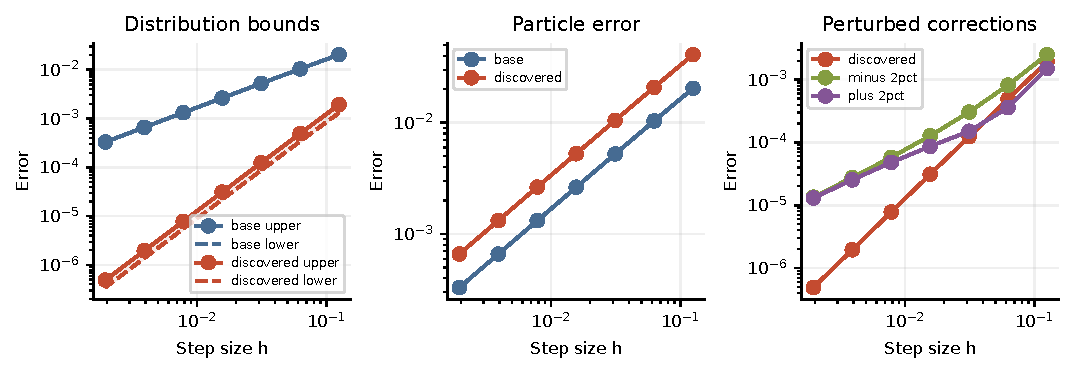
\includegraphics[width=\textwidth]{../results/revision/harmonic_convergence.pdf}
\caption{Nonradial correction discovery followed by fixed-field refinement. Left: quadrature evaluations of lower and upper bounds on full $W_2$, with the region between them shaded. Center: common-start particle RMS. Right: fixed $2\%$ perturbations of the discovered rotation restore an approximately first-order distribution-error trend. The corrected upper bound uses measure-preserving label rotation, not a same-start particle comparison.}
\label{fig:revision-convergence}
\end{figure*}

\paragraph{Residuals, infeasibility, and model error.}
Changing $\omega$ by $-2\%$ or $+2\%$ gives exact residual upper certificates $0.01345$ and $0.01372$ at $T$, and the finest observed upper-bound orders become $1.036$ and $0.961$. On the infeasible Gaussian path $\Sigma_t=\operatorname{diag}(1+t,1+t+2t^2)$, the scalar energy budget is positive throughout $[0,1]$, whereas the first coordinate gives the all-field lower bound $\varepsilon_t\ge[4(1+t)^{3/2}]^{-1}$. A separate one-coefficient noisy velocity regression over three seeds has analytically known learned paths. Refining Euler reduces its integration error while target error approaches the nonzero continuous-path error. This is a restricted parametric learning check, not a neural generative-model benchmark.

\paragraph{Cost and unfavorable baselines.}
Table~\ref{tab:revision-cost} preserves the comparison at $384$ field evaluations. Heun's evaluated upper bound is slightly below corrected Euler's evaluated lower bound, providing numerical evidence that Heun is more accurate on this path. RK3 is substantially better. Batch runtimes are comparable, and every stage pays for the inverse map; no sampling speedup is established. The correction improves Euler's distribution order, but it is not the best solver in this experiment. Supplement Section~\ref{sec:revision-experiments-details} gives timings, inverse tolerances, refinement data, optimizer failures, model-error floors, and reproduction commands.

\begin{table}[t]
\centering
\caption{Nonradial path at equal $384$ field evaluations. These are quadrature evaluations of continuum $W_2$ bounds.}
\label{tab:revision-cost}
\scriptsize
\begin{tabular}{@{}lrrr@{}}
\toprule
Method & $W_2$ lower & $W_2$ upper & Particle RMS\\
\midrule
Corrected Euler & $6.111\times10^{-7}$ & $8.675\times10^{-7}$ & $8.810\times10^{-4}$\\
Base Heun & $6.073\times10^{-7}$ & $6.085\times10^{-7}$ & $6.085\times10^{-7}$\\
Base RK3 & $1.067\times10^{-9}$ & $1.070\times10^{-9}$ & $1.070\times10^{-9}$\\
\bottomrule
\end{tabular}

\end{table}


\section{Established examples and solver trade-offs}
\label{sec:established-comparison}

The Gaussian and nonlinear radial positive controls are retained with their complete proofs and numerical receipts in the supplement. For $p_t=\mathcal N(0,e^{2at}I_2)$, the base field $ax$ and the corrected field $a(I+J)x$ have identical exact marginals. The correction changes Euler's $W_2$ error from first to second order and doubles the leading common-start particle-error coefficient. With $N$ uniform Euler steps and $N/2$ base-field Heun steps, both methods use $N$ evaluations and have exactly identical Gaussian output distributions at their shared grid points (Proposition~\ref{prop:equal-nfe}). Thus this example does not show an advantage over using a second-order solver.

For the shape-changing radial field $\alpha(r)x$, where
$\alpha(r)=a+\eta r^2/(1+r^2)$, the correction
$\beta(r)Jx$ with $\beta^2=\alpha^2+\alpha r\alpha'$ cancels radial acceleration. Theorem~\ref{thm:nonlinear} proves strict distribution-error improvement on every grid and positive first-order base, second-order corrected distribution, and first-order corrected particle constants. In the retained mixture example the particle coefficient increases by approximately $1.93$. At equal NFE corrected Euler has only $3.3$--$4.7\%$ smaller distribution error than base Heun; this does not imply lower wall-clock cost.

A correction is solver-specific. For $(aI+bJ)x$, Heun's leading distribution coefficient is proportional to $|a^3-3ab^2|$. The Euler choice $b=a$ worsens that coefficient relative to $b=0$; the distinct choice $b=a/\sqrt3$ gives third-order distribution accuracy with second-order particle accuracy. Existing equal-NFE Heun/RK3 comparisons and all unfavorable particle results are retained. A fixed radial rotation mismatch restores first-order distribution error in the proven examples, although terminal cancellations can occur on other paths. Local necessity and a uniform-grid terminal-cancellation example are given in Appendix~\ref{app:local}.

\section{Relation to previous work}
\label{sec:related}

Gauge freedom, weighted-gradient decompositions, and action minimization on a prescribed path are established in transport geometry and generative modeling~\citep{ambrosio2005gradient,liu2022marginal,horvat2024gauge,neklyudov2023action,paohuang2026flux}. The Gaussian rotation family is also known~\citep{lim2025hidden}. We do not claim the stream-function representation, the Hilbert projection theorem, or the convex chain rule as new. The constructive contribution is the reference-coordinate acceleration equation, its globally regular harmonic realization beyond affine-radial/product laws, and the exact correction certificate in that family. The strict quartic-observable counterexample supplies information not contained in scalar or covariance tests.

Hurault, Moreau, and Peyr\'e~\citep[Theorem~1 and Eq.~(4), v2]{hurault2026geometry} give weak Euler--Maruyama expansions for general smooth reverse diffusions, and specialize them to mean, covariance, and Fr\'echet errors. In their deterministic formula the propagated material acceleration controls the leading weak defect; our acceleration condition cancels it. The v2 analysis also develops Gaussian scale-mixture and parameter-selection expansions. Such weak and fitted-Gaussian discrepancies are distinct from full $W_2$ between non-Gaussian laws. Our finite-time coupling and projected-residual bounds control that full distance. The local coefficient theorem is a quantitative specialization of Wasserstein tangent geometry to Euler's defect, not a claim that tangent projection itself is new.

Tao and Choi~\citep{tao2026strain} analyze numerical particle error through strain, vorticity, and acceleration. Their same-start pairing cannot remove the leading rotation error in our examples. Rectified-flow re-pairing and kinetic path design can change intermediate distributions~\citep{liu2023flowstraight,pooladian2023multisample,tong2024otcfm,shaul2023kinetic}; our corrections preserve the stated path exactly. Bespoke solvers change the integrator~\citep{shaul2024bespoke}, while exponential solvers exploit a chosen linear part~\citep{zhang2023deis,lu2022dpmsolver}. A matrix exponential is already exact for the constant linear Gaussian example.

Huang et al.~\citep{huang2025divergence} connect flow-matching and divergence losses to continuous-path error in total variation. That objective concerns velocity/path fidelity, rather than the projected material acceleration that controls Euler's integration defect here. Beyler and Bach~\citep{beyler2025convergence} combine discretization, initialization, and score error in Wasserstein bounds for diffusion samplers, including Heun. Our target-path theorem uses a related stability principle while retaining the acceleration-projection cancellation. Convexity criteria for functionals on Wasserstein space~\citep{parker2024convexity} and higher invariant-measure orders for stochastic integrators~\citep{abdulle2014invariant,debussche2012weak} are related background; neither is identified with our nonzero, distribution-preserving material acceleration on a changing path.

Recent work on Neural Wasserstein Splines~\citep{banerjee2026splines} projects velocity and differentiates the moving projection to describe intrinsic Wasserstein acceleration. Our residual instead projects the material acceleration of the particular field being integrated. It is representation dependent, as the expanding Gaussian comparison demonstrates, and measures Euler's defect rather than an intrinsic acceleration of the marginal curve. The construction uses angular Fourier harmonics; it does not assert that its maps are spatially harmonic.

\section{Discussion and limitations}

The revised theory separates four regimes. Exact feasibility is demonstrated by the harmonic, Gaussian, and radial constructions. Certified approximation is described by upper residual bounds and the mixed $O(H^2)+O(\varepsilon H)$ guarantee. Proven infeasibility follows from convex-observable or covariance violations and can yield a strictly positive residual floor. For a general externally specified path, feasibility can remain unknown even when every tested moment condition passes.

The nonradial construction resolves the absence of an example beyond affine and product symmetry within a precise class; it does not establish a universal correction procedure. Its inverse-coordinate evaluation is additional computational work. A finite projection or small divergence penalty alone does not certify a small canonical residual. A correction selected separately as $H$ changes yields a statement about a uniformly controlled family, rather than second-order accuracy of one fixed learned field. The learned-path theorem requires regularity, moments, and a controlled mixed jerk term in addition to training loss. Global Lipschitz constants can make the bounds conservative.

The experiments support a mathematical mechanism and its certificates. They do not establish a practical speedup over Heun or RK3, scalable optimization for neural velocity fields, or improvements on image-generation benchmarks. Common-start particle errors remain important for inversion, editing, and paired transport. The new Gaussian-start variant, broader harmonic families, and efficient correction methods for externally given paths warrant further investigation.

\section*{Acknowledgment and AI assistance}
Artificial intelligence tools assisted the original preprint with mathematical analysis, literature review, code, and writing. This revision used OpenAI ChatGPT (GPT-6 Astra) for the feasibility, construction, certification, and new experimental sections, their supplementary proofs, the experimental code, and revised prose. Its roles included mathematical development, proof cross-checks, literature screening, software generation, numerical validation, and editing. The accompanying reproducibility report distinguishes analytical proofs, floating-point checks, and untested scope. These checks are not a formal proof-assistant certificate or independent human peer review. The author is responsible for validating the content before submission; this draft does not assert that the author has already independently verified the newly added results.

\bibliographystyle{IEEEtran}
\bibliography{references}
\clearpage
\onecolumn
\section*{Supplementary material}
\label{sec:supplement-start}
The following supplement contains the complete proofs, retained established results, numerical definitions, and additional validation details. The main paper and this supplement are also provided as one continuously referenced manuscript.
\appendices
\setcounter{theorem}{0}
\renewcommand{\thetheorem}{S\arabic{theorem}}
\renewcommand{\theHtheorem}{S\arabic{theorem}}
\section{Proofs and additional details of the harmonic construction}
\label{app:harmonic-proofs}

\subsection{Reference coordinates and path preservation}

Let $\rho$ be a probability measure and let a globally defined smooth
flow generated by $b$ preserve $\rho$. For a proper smooth diffeomorphism
$F_t$, the pushforward vector field $w_t(F_tz)=DF_t(z)b(z)$ has zero
weighted divergence under $(F_t)_\#\rho$. Indeed,
\[
 \int\nabla\phi(F_tz)\cdot DF_t(z)b(z)\,\rho(\dd z)
 =\int\nabla(\phi\circ F_t)(z)\cdot b(z)\,\rho(\dd z)=0.
\]
Properness makes the pulled-back test compactly supported. The exact
flow of $w_t$ at frozen physical time is the conjugate of the flow of
$b$ by $F_t$. For $u_t(F_tz)=\partial_tF_tz$, material differentiation
along a fixed reference label yields
$\acc_t(F_tz)=\partial_{tt}F_tz$ and
$\jerk_t(F_tz)=\partial_{ttt}F_tz$.
Equation~\eqref{eq:reference-acceleration} therefore suffices exactly.

More generally, for a time-dependent scalar $\gamma(t)$, the field
$\partial_tF_t+\gamma(t)DF_tJz$ has trajectories
$F_t(R_{\int_0^t\gamma(s)\dd s}z)$, where $R_\theta z=e^{i\theta}z$.
For a radial reference law all these fields generate the same $p_t$.
In Eq.~\eqref{eq:harmonic-gauge}, $\gamma=\omega-a$.
Only the constant-$\omega$ family is used for the polynomial search.

\subsection{Global diffeomorphism, density, and regularity}

The differential of $f(z)=z^2e^{-|z|^2}$ in any unit real direction
$\xi$ obeys
\[
 |Df(z)\xi|
 \le 2|z|(1+|z|^2)e^{-|z|^2}\le4/e.
\]
The last scalar function is maximal at $|z|=1$, as follows by
differentiating it; its derivative has the sign of
$1+r^2-2r^4$. Hence
\begin{align*}
 |F_t(z)-F_t(y)|
 &\ge e^{at}(1-q)|z-y|,\\
 |F_t(z)-F_t(y)|
 &\le e^{at}(1+q)|z-y|.
\end{align*}
For every $x$ the map $z\mapsto A_t^{-1}(x-B_tf(z))$ is a contraction
of the complete space $\R^2$ with constant at most $q<1$. Its unique
fixed point proves surjectivity and gives the inverse. The differential
is nonsingular everywhere; the inverse function theorem gives a smooth
inverse. The singular values of $DF_t$ are between
$e^{at}(1-q)$ and $e^{at}(1+q)$. The determinant is positive, because
the perturbation may be continuously reduced to zero without crossing
a singular differential. The density formula in the main text follows
by change of variables.

Every derivative of $f$ is a polynomial times $e^{-|z|^2}$. It and its
products with any fixed power of $|z|$ are bounded. On a neighborhood
of the compact time interval, the strict inequality $q<1$ persists
after a small extension of the interval. The inverse maps have uniformly
bounded first derivative, and bounded higher derivatives of each fixed
order. Consequently each of $u_a$ and $\acc_{u_a}$ is a fixed linear
field plus a smooth bounded perturbation with bounded first derivatives.
They are globally Lipschitz, have at most linear growth, and the required
time derivatives exist on this neighborhood. Explicitly,
\[
 \acc_{u_a}(t,F_tz)=2ia^2A_tz+4ia^2B_tf(z),\qquad
 \jerk_{u_a}(t,F_tz)
 =((1+i)a)^3A_tz+((1+i)a\sqrt2)^3B_tf(z).
\]
Their $L^2(p_t)$ norms are uniformly finite. The same smoothness and
growth conclusions hold for each fixed $u_\omega$, and uniformly for
$\omega$ in compact sets. Gaussian moments give all the integrability
needed for the later Taylor and moment arguments. This proves the
regularity part of Theorem~\ref{thm:harmonic-construction}.

For the multi-mode extension, the sum of Lipschitz perturbation bounds
is strictly less than the leading linear singular value by hypothesis.
The same contraction argument applies. Angular equivariance gives
$\partial_\theta f_n=in f_n$, while
$\partial_{tt}(e^{(1+i)a\sqrt n t}f_n)=2ia^2n
e^{(1+i)a\sqrt n t}f_n$. Thus
$F_{tt}=2a^2F_\theta$ persists. Rapid decay of the $f_n$ and all their
derivatives, and finiteness of the sum, give the same regularity bounds.

\subsection{Why the example is neither affine-radial nor affine-product}

For a standard planar Gaussian $Z$, angular orthogonality gives
\begin{align}
 \E F_t(Z)&=0,\qquad \E F_t(Z)^2=0,\qquad \E F_t(Z)^3=0,
 \label{eq:harmonic-oddmoments}\\
 \E\bigl[F_t(Z)^2\overline{F_t(Z)}\bigr]
 &=A_t^2\overline B_t\,\E[|Z|^4e^{-|Z|^2}]
 =\frac8{27}A_t^2\overline B_t\ne0.\nonumber
\end{align}
Also $\E|F_t(Z)|^2=2|A_t|^2+(8/125)|B_t|^2$, so the real covariance
is a positive multiple of $I_2$. An affine image of a radial law is
centrally symmetric about its mean, which would make the last cubic
moment zero. Thus no such representation exists.

Suppose instead that the centered real vector $F_t(Z)$ were an
invertible affine image of independent scalar variables. Finite third
moments follow from those of $F_t(Z)$ and the inverse affine map.
After centering and standardizing the independent variables, isotropic
covariance forces the remaining mixing matrix to be a scalar multiple
of an orthogonal matrix. For independent centered real $U,V$,
\[
 \E(U+iV)^3=\E U^3-i\E V^3,\qquad
 \E[(U+iV)^2(U-iV)]=\E U^3+i\E V^3.
\]
The two quantities therefore have equal moduli. Orthogonal rotations,
reflections, and common scaling preserve this equality of moduli.
Equation~\eqref{eq:harmonic-oddmoments} violates it. This rules out an
affine-product representation, proving the final assertion of the
theorem. The small deformation is consequently not one of the earlier
radial, Gaussian, affine-radial, or independent-product constructions.

For Corollary~\ref{cor:gaussian-start}, the proposed bound is a uniform
upper bound on $(4/e)|B_t/A_t|$, because $e^{-at}\le1$ and
$|\sinh((1+i)a\sqrt2t)|\le\sqrt2\sinh(a\sqrt2T)$.
The diffeomorphism and regularity proofs therefore apply unchanged.
The second-derivative identity still holds, $B_0=0$, and $B_t\ne0$ for
$t>0$ since its real argument is positive. The moment argument above
continues to apply with this coefficient. This proves the corollary.

\subsection{Exact residual polynomial and correction recovery}

Along the $u_\omega$ trajectories the reference label rotates at rate
$\omega-a$. The material derivative on functions of $(t,z)$ is
$\partial_t+(\omega-a)\partial_\theta$. Applying it twice to each
$F_{n,t}$ gives the coefficient $\zeta_n^2$ in the main text.
Angular orthogonality makes different harmonics orthogonal in complex
$L^2(\rho)$, which is the real vector $L^2$ norm. Since
$|Z|^2$ has density $\tfrac12e^{-s/2}$ on $[0,\infty)$,
\[
 \E|Z|^2=2,\qquad
 \E[|Z|^4e^{-2|Z|^2}]
 =\frac12\int_0^\infty s^2e^{-5s/2}\dd s=\frac8{125}.
\]
This proves Eq.~\eqref{eq:harmonic-residual}. The first mode is
$\zeta_1=a+i\omega$. Its squared real part is $a^2-\omega^2$, so a
zero residual requires $\omega=\pm a$ and $c=2a\omega$.
If $\omega=-a$, the second mode has real part of its squared
coefficient $2a^2-a^2(\sqrt2-4)^2\ne0$. If $\omega=a$, both mode
coefficients equal $inc$ for $c=2a^2$. As all $M_n$ are positive,
these alternatives prove uniqueness of the zero.

For fixed $\omega$, differentiate the quadratic objective in $c$ to
obtain $c_*$. The imaginary part of $\zeta_n^2$ is affine in $\omega$,
so eliminating $c$ changes only terms of degree at most two in
$\omega$. The real squared coefficients contribute the positive
quartic leading term $\sum n^4M_n$. Coercivity and differentiation
therefore give the finite global minimization procedure. The same
calculation applies to time integrals, because the coefficients
$\zeta_n$ are time-independent. This proves
Proposition~\ref{prop:harmonic-search}.

The upper certificate controls the canonical projected residual by
orthogonal projection. It need not equal that residual away from the
recovered zero, because a single solenoidal basis field need not be the
best approximation among all solenoidal fields. The proof certifies
the exact algebraic solution $\omega=a,c=2a^2$; machine residuals near
roundoff describe a numerical recovery of this solution.

\subsection{A finite modified-flow argument for the explicit coupling}

Let $u=u_a$ and $\acc=\acc_u$. For each $0<h\le h_0$, define
$u_h=u-(h/2)\acc$. The curve
\[
 Y_h(t,z)=F_t(e^{-ia^2ht}z)
\]
solves $\dot Y_h=u_h(t,Y_h)$ and starts from $F_0(z)$.
For $Z\sim\rho$, its law at each $t$ is exactly $p_t$.
On a fixed bounded range of $h$, $u_h$ and its required derivatives
satisfy uniform linear-growth and spatial Lipschitz bounds by the
previous regularity calculation. Its material acceleration is
\[
 \partial_tu_h+(D u_h)u_h
 =\acc-\frac h2\{\jerk+(Du)\acc\}
       +\frac{h^2}4(D\acc)\acc,
\]
All remainder terms have an $L^2$ bound proportional to
$1+|z|$ along $Y_h$, uniformly in $h$ and $t$; the third derivatives
needed for the Taylor remainder have the same bound. Taylor expansion
over one step gives
\begin{align*}
 Y_h(t+h,z)
 &=Y_h(t,z)+h[u(t,Y_h)-(h/2)\acc(t,Y_h)]\\
 &\quad+\frac{h^2}2\acc(t,Y_h)
       +O_{L^2(\rho)}(h^3)\\
 &=Y_h(t,z)+h u(t,Y_h(t,z))+O_{L^2(\rho)}(h^3).
\end{align*}
Minkowski's inequality and Euler stability imply
$e_{k+1}\le(1+Lh)e_k+Ch^3$, where
$e_k=\|\widehat X_k-Y_h(t_k,Z)\|_{L^2}$ and $e_0=0$.
Summing yields $\max_ke_k\le CT e^{LT}h^2$. Because rotations preserve
$\rho$, the pairing at $t=T$ proves
Eq.~\eqref{eq:harmonic-coupling}.

Finally, Taylor expansion in the rotation angle gives in $L^2(\rho)$
\[
 F_T(e^{-ia^2Th}Z)
 =F_T(Z)-a^2Th\,DF_T(Z)JZ+O_{L^2}(h^2).
\]
The preceding $O(h^2)$ coupling error therefore shows
$h^{-1}(\widehat X_N-F_T(Z))\to-a^2TDF_T(Z)JZ$ in $L^2$.
Taking norms proves Eq.~\eqref{eq:harmonic-particle-limit}. Its constant
is positive since $DF_T$ is nonsingular and $\rho(Z=0)=0$.
For a uniform grid the same argument works at every grid point with
$T$ replaced by $t_k$. The law-level $O(H^2)$ assertion for arbitrary
grids is supplied separately by Theorem~\ref{thm:distribution_order}.

\section{Proofs for residual certification and target-path stability}
\label{app:certification-proofs}

\subsection{Projection and the weighted weak problem}

The space $L^2(p;\R^d)$ is Hilbert, and $\mathcal G_p$ is closed by
definition.  The Hilbert projection theorem therefore gives a unique
$g=\Pi_pa$.  Its complement $w=a-g$ satisfies
$\int w\cdot\nabla\phi\,\dd p=0$ for every smooth compactly supported
$\phi$.  Conversely this identity places $w$ in $\mathcal G_p^\perp$.
Taking a supremum over a dense set of unit gradients proves
Eq.~\eqref{eq:canonical-residual}.  This argument makes no regularity
claim about $g$ or $w$.

For a smooth positive density with a Poincar\'e constant $C_P$, the
projection has a potential, unique modulo constants, satisfying
\begin{equation}
 \int\nabla\varphi\cdot\nabla\eta\,p\,\dd x
   =\int a\cdot\nabla\eta\,p\,\dd x,
 \qquad -\nabla\cdot(p\nabla\varphi)=-\nabla\cdot(pa).
 \label{eq:weighted-poisson-certificate}
\end{equation}
The potential is understood in the completion of centered smooth test
functions in weighted $H^1$.  On $\R^d$ this is a finite-energy weak problem;
no unmentioned boundary condition at a numerical truncation boundary is
imposed.  If an exact Galerkin $q_N$ has strong residual
$d_N=p^{-1}\nabla\cdot[p(a-q_N)]\in L^2(p)$ with zero mean, then
\begin{equation}
 \|q_N\|_{L^2(p)}^2\le\|\Pi_pa\|_{L^2(p)}^2
 \le\|q_N\|_{L^2(p)}^2+C_P\|d_N\|_{L^2(p)}^2.
 \label{eq:poisson-residual-upper}
\end{equation}
This explains precisely when a divergence penalty gives an upper bound:
the weighted norm, the Poincar\'e constant, and the weak residual identity
must all be controlled.

Numerical integration error must also be enclosed.  If computed values
$\widehat{\mathcal L},\widehat{\mathcal U}$ have deterministic error bounds
$\eta_L,\eta_U$, and the acceleration supplied to those computations differs
from the true acceleration by at most $\delta_a$ in $L^2(p)$, then
\begin{equation}
 \max\!\left\{0,\sqrt{\max(0,\widehat{\mathcal L}-\eta_L)}-\delta_a\right\}
 \le\|\Pi_pa\|
 \le\sqrt{\max(0,\widehat{\mathcal U}+\eta_U)}+\delta_a.
 \label{eq:inexact-certificate}
\end{equation}
Here the primal and dual fields must be admissible for the same exact
$p$.  Sample standard errors alone are not deterministic quadrature
certificates; confidence bounds give statements with their specified
coverage.

For the potential formulation, assume $p$ is a smooth positive density
with $\|\eta-\E_p\eta\|_{L^2(p)}^2\le
C_P\|\nabla\eta\|_{L^2(p)}^2$.  Complete the centered functions $f-\E_pf$, with $f\in C_c^\infty$,
in the weighted $H^1$ norm.  The gradient norm is
equivalent to that norm on this centered space.  The form
$\int\nabla\varphi\cdot\nabla\eta\,p\,\dd x$ is continuous and
coercive, and the functional $\int a\cdot\nabla\eta\,p\,\dd x$ is
bounded.  The Hilbert-space representation theorem yields a unique
centered $\varphi$ with Eq.~\eqref{eq:weighted-poisson-certificate}.
Its gradient is the projection.  Other representatives differ by a
constant within the uncentered completion.

For an exact Galerkin solution, $g-q_N$ is orthogonal to the finite
gradient space and hence to $q_N$.  If the stated strong residual exists,
then for centered tests
\[
 \langle g-q_N,\nabla\eta\rangle
   =-\int d_N\eta\,\dd p
   \le\sqrt{C_P}\|d_N\|_{L^2(p)}\|\nabla\eta\|_{L^2(p)}.
\]
Density gives $\|g-q_N\|\le\sqrt{C_P}\|d_N\|$.  Pythagoras proves
Eq.~\eqref{eq:poisson-residual-upper}.  The same argument applied to
$p^{-1}\nabla\cdot(pr)$ proves Eq.~\eqref{eq:score-path-defect}; compact
support removes boundary terms and implies zero mean of this divergence.

Finally, using an approximate density has a measurable cost.  If
$r=\widetilde p^{-1}J\nabla\psi$ has compact support, then
\[
 p^{-1}\nabla\cdot(pr)
 =r\cdot(\nabla\log p-\nabla\log\widetilde p).
\]
When $p$ has Poincar\'e constant $C_P$, integration by parts gives
\begin{equation}
 \|\Pi_pr\|_{L^2(p)}
 \le\sqrt{C_P}\,
 \|r\cdot(\nabla\log p-\nabla\log\widetilde p)\|_{L^2(p)}.
 \label{eq:score-path-defect}
\end{equation}
Thus a score approximation controls a path-defect term under explicit
norm and Poincar\'e assumptions; it does not preserve the exact target
path automatically.

\begin{proof}[Proof of Proposition~\ref{prop:residual-certificates}]
Write $a=g+z$ with $g=\Pi_pa$ and $z\in\mathcal G_p^\perp$.  Orthogonality
gives
\[
 \|g\|^2-\mathcal L=\|g-q\|^2,\qquad
 \mathcal U-\|g\|^2=\|z-w\|^2.
\]
Their sum is $\|g-q+z-w\|^2=\|a-w-q\|^2$.  For an exact Galerkin
solution, $\langle a,q_N\rangle=\|q_N\|^2$, giving the stated matrix
formula.  For Eq.~\eqref{eq:inexact-certificate}, first enclose the
certificate for the approximate acceleration.  Orthogonal projection is
contractive, so changing that acceleration by $\delta_a$ changes its
projected norm by at most $\delta_a$.
\end{proof}

\subsection{A quantitative flow lemma requiring no solenoidal flow}

We use the standard continuity-equation estimate
\begin{equation}
 W_2(\mu_b,\mu_a)\le\int_a^b\|V_s\|_{L^2(\mu_s)}\,\dd s
 \quad\text{if}\quad
 \partial_s\mu_s+\nabla\cdot(\mu_sV_s)=0,
 \label{eq:ce-length}
\end{equation}
for narrowly continuous finite-second-moment curves and integrable
$L^2$ velocities~\citep[Theorem~8.3.1]{ambrosio2005gradient}.  The
estimate requires neither uniqueness nor classical trajectories for
$V_s$.  All curves constructed below are continuous pushforwards by
globally Lipschitz diffeomorphisms, so their continuity and moment
conditions hold.

\begin{lemma}[Frozen flow displacement controlled by projection]
\label{lem:projected-frozen-flow}
Let $p\in\mathcal P_2(\R^d)$ and let $a\in C^1(\R^d;\R^d)$ be globally
$L_a$-Lipschitz, with $a\in L^2(p)$.  Write $\Phi^s$ for its autonomous
flow and set
\[
 Q_a(\tau)=\int_0^\tau e^{L_as}\,\dd s
 =\begin{cases}(e^{L_a\tau}-1)/L_a,&L_a>0,\\\tau,&L_a=0.
 \end{cases}
\]
For every $\tau\ge0$,
\begin{equation}
 W_2((\Phi^\tau)_\#p,p)
 \le Q_a(\tau)\|\Pi_pa\|_{L^2(p)}.
 \label{eq:frozen-projected-bound}
\end{equation}
\end{lemma}

\begin{proof}
Let $g=\Pi_pa$ and $w=a-g$.  On $0\le s\le\tau$, define
$\mu_s=(\Phi^{\tau-s})_\#p$ and, with $y=\Phi^{\tau-s}(x)$,
\[
 V_s(y)=-D\Phi^{\tau-s}(x)g(x).
\]
For a compactly supported smooth test $f$, differentiating its integral
under $\mu_s$ initially gives the same expression with $a$ instead of
$g$.  The omitted term is
$\int \nabla(f\circ\Phi^{\tau-s})(x)\cdot w(x)\,p(\dd x)=0$.
The composition is $C^1$ and compactly supported; convolution extends
the defining orthogonality from smooth tests to these tests.  Here
$D\Phi^r(x)a(x)=a(\Phi^r(x))$, the autonomous flow identity, gives
the differentiated expression.  Thus $(\mu_s,V_s)$ satisfies the
continuity equation.  Moreover
\[
 \|V_s\|_{L^2(\mu_s)}
 \le e^{L_a(\tau-s)}\|g\|_{L^2(p)}.
\]
Apply Eq.~\eqref{eq:ce-length} between
$\mu_0=(\Phi^\tau)_\#p$ and $\mu_\tau=p$.
The proof never constructs a flow for $w$.
\end{proof}

\begin{proof}[Proof of Theorem~\ref{thm:projected-residual}]
Fix $t$ and an admissible step $h$, write $X\sim p_t$, and set
$\tau=h^2/2$.  For the frozen acceleration flow, the elementary
Gronwall estimate
$\|\acc_t(\Phi^sX)\|_{L^2}\le e^{L_as}\|\acc_t(X)\|_{L^2}$ gives
\begin{align*}
 \|\Phi^\tau X-X\|_{L^2}&\le Q_a(\tau)C_a,\\
 \|\Phi^\tau X-X-\tau\acc_t(X)\|_{L^2}
   &\le \tfrac12L_aC_a\tau^2e^{L_a\tau}.
\end{align*}
For completeness, the first pointwise estimate follows by writing
$a(\Phi^s x)=a(x)+\int_0^sDa(\Phi^r x)a(\Phi^r x)\,\dd r$ and
using $\|Da\|_{\rm op}\le L_a$.  The second bound follows by
integrating $\|a(\Phi^sX)-a(X)\|\le L_a\|\Phi^sX-X\|$.

The exact physical flow has expansion
\[
 F_{t,t+h}X=X+hu_t(X)+\tfrac12h^2\acc_t(X)+R,
 \qquad \|R\|_{L^2}\le C_jh^3/6.
\]
The actual marginal at intermediate physical time is $p_s$, which
justifies the $C_j$ bound under the integral Taylor remainder.
Consequently, for $E_{t,h}(x)=x+hu_t(x)$,
\begin{align*}
 \|E_{t,h}(\Phi^\tau X)-F_{t,t+h}X\|_{L^2}
 &\le C_jh^3/6+hLC_aQ_a(\tau)
       +\tfrac12L_aC_a\tau^2e^{L_a\tau}\\
 &\le D_Hh^3.
\end{align*}
The remaining change of input distribution is bounded by
Lemma~\ref{lem:projected-frozen-flow} and the Euler Lipschitz constant:
\[
 W_2((E_{t,h})_\#p_t,
       (E_{t,h})_\#(\Phi^\tau)_\#p_t)
 \le(1+Lh)Q_a(\tau)\varepsilon_t
 \le\tfrac12B_Hh^2\varepsilon_t.
\]
The triangle inequality gives the local bound.  The recurrence
$e_{k+1}\le(1+Lh_k)e_k+D_Hh_k^3+B_Hh_k^2\varepsilon_{t_k}/2$,
with $e_0=0$, proves Eq.~\eqref{eq:projected-bound} after multiplication
by the later stability factors and use of
$\prod_k(1+Lh_k)\le e^{LT}$.
\end{proof}

\begin{proof}[Proof of Corollary~\ref{cor:sharp-local-residual}]
Fix $t<T$ and let $\mu_h=(E_{t,h})_\#p_t$, $\nu_h=p_{t+h}$, and
$d_h=W_2(\mu_h,\nu_h)$.  The single-step estimate proved above gives
$\limsup_{h\downarrow0}d_h/h^2\le\varepsilon_t/2$.
In particular $d_h=O(h^2)$, and $\mu_h\to p_t$ in $W_2$ because
$\|E_{t,h}X-X\|_{L^2}=h\|u_t\|_{L^2(p_t)}$.

For $\phi\in C_c^\infty$, Taylor expansion in an optimal coupling
of $\mu_h$ and $\nu_h$ and Cauchy--Schwarz give
\[
 \left|\int\phi\,\dd\nu_h-\int\phi\,\dd\mu_h\right|
 \le\|\nabla\phi\|_{L^2(\mu_h)}d_h
       +\tfrac12\|D^2\phi\|_\infty d_h^2.
\]
The same-start Taylor expansion used for local necessity gives
\[
 \int\phi\,\dd\nu_h-\int\phi\,\dd\mu_h
 =\tfrac12h^2\langle\acc_t,\nabla\phi\rangle_{L^2(p_t)}+o(h^2).
\]
This expansion needs only the stated $L^2$ acceleration and jerk bounds:
replace the exact-minus-Euler displacement by $h^2\acc_t(X)/2$
with an $L^2$ remainder $O(h^3)$, and use bounded first and second
derivatives of $\phi$.
Since $\|\nabla\phi\|_{L^2(\mu_h)}\to
\|\nabla\phi\|_{L^2(p_t)}$, division by $h^2$ gives, whenever the
latter norm is positive,
\[
 \liminf_{h\downarrow0}\frac{d_h}{h^2}
 \ge\frac{|\langle\acc_t,\nabla\phi\rangle_{L^2(p_t)}|}
            {2\|\nabla\phi\|_{L^2(p_t)}}.
\]
The supremum over these tests is $\varepsilon_t/2$ by
Eq.~\eqref{eq:canonical-residual}.  If $\varepsilon_t=0$, the upper
bound and nonnegativity suffice.  This proves the limit, including
singular $p_t$, without requiring an optimal transport map.
\end{proof}

\subsection{Regularity and optimization of compact gauges}

\begin{proposition}[Compact gauge search]
\label{prop:compact-gauge-search}
Suppose $p_t$ is a strictly positive $C^4$ density and is generated by a
field $v$ satisfying the regularity and moment bounds of
Theorem~\ref{thm:projected-residual}.  Let the $C^4$ potentials in
Eq.~\eqref{eq:compact-stream-gauge} have spatial support in one compact set
$K$, uniformly in time, and let $\theta$ range over a compact set
$\Theta\subset\R^m$.  Then $u_\theta=v+r_\theta$ has a global flow
generating exactly $p_t$.  The regularity and moment constants in
Theorem~\ref{thm:projected-residual} can be chosen uniformly on $\Theta$.
The objective
\begin{equation}
 \mathcal E(\theta)=\sup_{0\le t\le T}
    \|\Pi_{p_t}[\partial_tu_\theta+(D_xu_\theta)u_\theta]\|_{L^2(p_t)}
 \label{eq:gauge-objective}
\end{equation}
is Lipschitz on $\Theta$ and attains its minimum.
If its Lipschitz constant is $K_\Theta$, a finite $\delta$-net of
$\Theta$, evaluated with certified upper and lower objective bounds of
width at most $\eta$, has a candidate $\widehat\theta$ chosen by its
smallest upper bound satisfying
\[
 \mathcal E(\widehat\theta)
 \le\min_{\theta\in\Theta}\mathcal E(\theta)+K_\Theta\delta+\eta.
\]
\end{proposition}

\begin{proof}[Proof of Proposition~\ref{prop:compact-gauge-search}]
Positivity and continuity of $p$ give a positive minimum on
$[0,T]\times K$.  Therefore $r_\theta$ and its derivatives through the
orders used below are bounded and have support in $K$, uniformly for
$\theta\in\Theta$.  The identity
$\nabla\cdot(J\nabla\psi)=0$ proves exact weighted divergence
freedom.  In higher dimensions, let $A_{ij}=-A_{ji}$ and set
$r_i=p^{-1}\sum_j\partial_jA_{ij}$. For this antisymmetric tensor, mixed partial
derivatives cancel in pairs in
$\sum_{ij}\partial_i\partial_jA_{ij}$.

The field $u_\theta$ is globally Lipschitz and has linear growth,
uniformly over $\Theta$.  Its global flow is therefore defined on the
whole interval.  The prescribed $p_t$ satisfies its continuity equation,
and uniqueness for a globally Lipschitz field shows that this is its
actual path.  The acceleration difference
\begin{equation}
 \acc_{u_\theta}-\acc_v
 =\sum_i\theta_i b_i+\sum_{ij}\theta_i\theta_jc_{ij},
 \quad
 b_i=\partial_tr_i+(D_xv)r_i+(D_xr_i)v,
 \quad c_{ij}=(D_xr_i)r_j,
 \label{eq:acceleration-parameter-polynomial}
\end{equation}
is supported in $K$ with uniformly bounded first derivatives.  Thus
the acceleration Lipschitz and $L^2$ bounds are uniform.  The jerk
difference is also compactly supported and bounded, because it uses
only the displayed regular derivatives and the locally bounded
derivatives of $v$.  This proves all uniform moment assertions.

Let $R=\sup_{\theta\in\Theta}\|\theta\|_2$,
$B=(\sum_i\sup_t\|b_i\|_{L^2(p_t)}^2)^{1/2}$, and
$C=(\sum_{ij}\sup_t\|c_{ij}\|_{L^2(p_t)}^2)^{1/2}$.
Equation~\eqref{eq:acceleration-parameter-polynomial} and
$\|\theta\otimes\theta-\eta\otimes\eta\|_2
\le2R\|\theta-\eta\|_2$ imply
\[
 \sup_t\|\acc_{u_\theta,t}-\acc_{u_\eta,t}\|_{L^2(p_t)}
 \le(B+2RC)\|\theta-\eta\|_2.
\]
Projection is contractive.  The reverse triangle inequality and then
the supremum over time prove Lipschitz continuity of $\mathcal E$ with
$K_\Theta=B+2RC$.  Compactness gives a minimizer $\theta_*$.  Choose
a net point $\theta_i$ within $\delta$ of $\theta_*$.  Its upper
certificate is at most
$\mathcal E(\theta_*)+K_\Theta\delta+\eta$; selecting the smallest
upper certificate proves the claimed bound.  This proof requires
certificates of the continuous-time supremum, not unqualified values
at sampled times.

For the time envelope, choose a computable $C^1$ field $w_t$ with zero
weighted divergence under the target and define $R_t=\acc_t-w_t$.
Assume $K_R=\sup_t\|\partial_tR_t+(D_xR_t)v_t\|_{L^2(p_t)}<\infty$.
Then $\varepsilon_t\le\|R_t\|$.  This regularity is imposed on the
chosen upper-certificate field, not on the orthogonal projection.
Couple $p_s$ and $p_t$ using the exact target flow.  The chain rule and
Minkowski's inequality give
\[
 \big|\|R_t\|_{L^2(p_t)}-\|R_s\|_{L^2(p_s)}\big|
 \le\int_s^t\|\partial_rR_r+(D_xR_r)v_r\|_{L^2(p_r)}\,\dd r.
\]
The bound $K_R|t-s|$ and the covering property of the time net give
the envelope $\sup_t\|R_t\|\le\max_i\|R_{s_i}\|+K_R\Delta$,
where $\Delta$ is the covering radius of the time net. A lower bound
for $\sup_t\varepsilon_t$ is the maximum of the lower certificates
at those nodes. Achieving uniformly vanishing bracket widths further
requires control of the primal--dual gaps; it is not a consequence of
time-grid refinement alone.
\end{proof}

\subsection{A target-measure stability estimate}

\begin{lemma}[Exact-flow comparison using the projected path defect]
\label{lem:projected-path-stability}
Under the path and field assumptions of Theorem~\ref{thm:target-path-bound},
for $s<t$,
\begin{equation}
 W_2((F^u_{s,t})_\#p_s,p_t)
 \le\int_s^t e^{L(t-r)}\beta_r\,\dd r.
 \label{eq:projected-path-stability}
\end{equation}
\end{lemma}

\begin{proof}
Set $b_r=\Pi_{p_r}(u_r-v_r)$ and
$\mu_r=(F^u_{r,t})_\#p_r$.  Differentiating a smooth compactly
supported test integral and using the target continuity equation gives
\[
 \frac{\dd}{\dd r}\int f\,\dd\mu_r
 =\int\nabla f(F^u_{r,t}x)\cdot
             D_xF^u_{r,t}(x)(v_r(x)-u_r(x))\,p_r(\dd x).
\]
The term $u_r-v_r-b_r$ has zero weighted divergence under $p_r$.
Testing it against $f\circ F^u_{r,t}$ replaces $v_r-u_r$ by $-b_r$.
This gives a continuity-equation velocity of $\mu_r$ with norm at most
$e^{L(t-r)}\beta_r$.  A Borel version of the projections may be
obtained by projecting onto an increasing countable family of smooth
gradient tests and taking the $L^2$ limit; the resulting weak identities
are sufficient here.  Equation~\eqref{eq:ce-length} proves the claim.
\end{proof}

\begin{proof}[Proof of Theorem~\ref{thm:target-path-bound}]
Start a single exact $u$-step from $X\sim p_{t_k}$.
The integral Taylor remainder is at most $C_j^\diamond h_k^3/6$ by
assumption.  All frozen-flow estimates in the proof of
Theorem~\ref{thm:projected-residual} therefore apply under this target
measure, giving
\[
 W_2((E^u_{t_k,h_k})_\#p_{t_k},
          (F^u_{t_k,t_{k+1}})_\#p_{t_k})
 \le D_Hh_k^3+\tfrac12B_Hh_k^2\varepsilon_{t_k}.
\]
Lemma~\ref{lem:projected-path-stability} bounds the difference between
the second law and $p_{t_{k+1}}$.  Consequently, with
$e_k=W_2(\widehat q_k,p_{t_k})$,
\[
 e_{k+1}\le(1+Lh_k)e_k+D_Hh_k^3
       +\tfrac12B_Hh_k^2\varepsilon_{t_k}
       +\int_{t_k}^{t_{k+1}}e^{L(t_{k+1}-s)}\beta_s\,\dd s.
\]
Iteration proves Eq.~\eqref{eq:target-path-bound}.  In fact the path
term can retain the smaller factor
$\int_0^{t_k}e^{L(t_k-s)}\beta_s\,\dd s$, since later Euler stability
factors are bounded by $e^{L(t_k-t_{j+1})}$.

To check the stated sufficient jerk condition, suppose
\[
 \|\jerk_u(s,x)\|\le J_0+J_1\|x\|,\qquad
 \sup_t\|u(t,0)\|\le U_0,\qquad
 \sup_t\E_{p_t}\|X\|^2\le M.
\]
The growth estimate
$\|F^u_{t,s}(x)\|\le e^{LT}(\|x\|+TU_0)$ yields
$C_j^\diamond\le J_0+J_1e^{LT}(\sqrt M+TU_0)$.
Finally, conditional expectation makes the cross term in the squared
regression loss zero.  Projection contraction and Cauchy--Schwarz in
time give $\int\beta_t\,\dd t\le\sqrt{T\mathcal R_{\rm excess}}$.
Linearity of $\Pi_{p_t}$ proves that a target-solenoidal correction
leaves $\beta_t$ unchanged.
\end{proof}

\section{Proofs of the path-level feasibility certificates}
\label{app:convex-feasibility}

\subsection{Convex observables and weighted kinetic energy}
\begin{proof}
Along an exact trajectory, two derivatives of $\phi(X_t)$ give
$u_t(X_t)^\top D^2\phi(X_t)u_t(X_t)+
\nabla\phi(X_t)\cdot\acc_t(X_t)$.
The global growth bounds and the finite second moment dominate these terms
when $D^2\phi$ is bounded.  Smooth compact cutoffs of $\phi$ have gradients
converging to $\nabla\phi$ in $L^2(p_t)$: both the gradient and the cutoff
error are bounded by $C(1+\|x\|)$, with the error supported in the tails.
Thus the acceleration condition removes the final integral in
\eqref{eq:convex-chain-rule}.  A convex Hessian makes the first integral
nonnegative.  Without that condition, the first integral is at least
$K_\phi(t)$, and the definition of $\varepsilon_t^{\rm acc}$ bounds the
absolute value of the final integral by
$\varepsilon_t^{\rm acc}\|\nabla\phi\|_{L^2(p_t)}$.  This proves
\eqref{eq:convex-residual-floor}.  The additional hypotheses stated for
unbounded tests justify the identical argument.
\end{proof}

The theorem implies the convex-order condition
\begin{equation}
 p_{(1-\lambda)s+\lambda t}
 \preceq_{\rm cx}(1-\lambda)p_s+\lambda p_t,
 \qquad 0\le s<t\le T,\quad 0\le\lambda\le1.
 \label{eq:convex-order-path}
\end{equation}
Here $\preceq_{\rm cx}$ compares expectations of convex functions, and the
right side is a mixture of endpoint measures.  To extend the proved
inequality beyond smooth tests, first mollify convex Lipschitz functions
and then approximate an arbitrary convex function from below by maxima of
finitely many supporting affine functions.  Subtracting one supporting
affine function permits monotone convergence; the mean is affine by
Corollary~\ref{cor:mean-action}.  This is a necessary condition, not an
existence theorem.  In particular, every straight stochastic interpolation
$\Law((1-t)X_0+tX_1)$ already satisfies the convex-observable test, regardless
of whether it has an acceleration-preserving deterministic generator.


For a smooth positive density, the weighted quantity $K_\phi$ has a linear
variational characterization.  If $B=D^2\phi$ satisfies $b_-I\preceq B\preceq b_+I$ for positive finite constants, a weighted Poincare
inequality and one finite-energy generating field give a solution $\chi$,
unique modulo constants in the weighted Sobolev completion of smooth
functions, of
\[
 \int \nabla\eta^\top B^{-1}\nabla\chi\,\dd p_t
 =\int\eta\,\partial_t p_t\,\dd x.
\]
Its velocity $v_\phi=B^{-1}\nabla\chi$ attains $K_\phi$.  Indeed, every other
admissible velocity differs by a zero-weighted-divergence field $r$, and
$\int r\cdot\nabla\chi\,\dd p_t=0$.  Expansion of the quadratic energy
proves minimality.  This permits a linear elliptic feasibility diagnostic
without asserting that the nonlinear correction problem is solvable.


\subsection{Covariance constraints and their limits}
\begin{proof}
Applying \eqref{eq:convex-chain-rule} to quadratic coordinate products,
or polarizing its quadratic-form identity, gives
$\frac{\dd^2}{\dd t^2}\E[X_tX_t^\top]=2\E[u_tu_t^\top]$.
Subtracting $m(t)m(t)^\top$ yields
$C''=2\E[(u_t-\xi)(u_t-\xi)^\top]$.
The displayed block matrix is the covariance of $(X_t,u_t(X_t))$.
For $Z=e\cdot(X_t-m(t))$ and $V=e\cdot(u_t(X_t)-\xi)$,
$q=\sigma_e^2$ satisfies $q'=2\E[ZV]$ and $q''=2\E[V^2]$.
Hence
\[
 \sigma_e''=
 \frac{\E[Z^2]\E[V^2]-(\E[ZV])^2}
 {(\E[Z^2])^{3/2}}\ge0
\]
by Cauchy--Schwarz.
\end{proof}

These tests form a strict hierarchy.  For example, a diagonal Gaussian
path with standard deviations $s_1(t)=1+t-t^2/10$ and
$s_2(t)=1+t+t^2$ on $[0,1/4]$ has positive $C''$ and passes the scalar
minimum-energy test, because
$M''/2-K_{\min}=s_1s_1''+s_2s_2''>0$.
It is nevertheless infeasible because $s_1''=-1/5<0$.
The next example also passes the full covariance test.


\subsection{The quartic obstruction and its residual floor}
\begin{proof}
The bounds $|\kappa|\le1$ and
$r|\kappa'(r)|\le5/(2e)<1$ give $\|Db\|_{\rm op}<2$.
Thus $G_t$ is a global smooth bi-Lipschitz map, with lower Lipschitz
constant at least $1-t^2\ge3/4$.  Its nonlinear terms have bounded
derivatives, and its inverse has uniformly bounded first derivatives on
the interval.  The generator and its material acceleration
$b\circ G_t^{-1}$ are globally Lipschitz.  The source is Gaussian and the
maps have linear growth, so every required moment is finite.  The generator
is radial, hence a gradient, with a potential of at most quadratic growth;
the weighted-gradient orthogonality argument establishes its minimum
kinetic energy.

For $R=\|Z\|$, $R^2/2$ is exponential with mean one, and
\[
 \E[R^{2\ell}e^{-jR^2/2}]
 =\frac{2^\ell\ell!}{(1+j)^{\ell+1}}.
\]
It follows exactly that
\[
 M(t)=2+\frac{t^2}{8}+\frac{23t^4}{576},\qquad
 K_{\min}(t)=\frac{23t^2}{144},\qquad
 M''-2K_{\min}=\frac14+\frac{23t^2}{144}>0.
\]
The mean is zero and $C(t)=q(t)I_2$, where
$q(t)=1+t^2/16+23t^4/1152$.
For $q=1+\alpha t^2+\beta t^4$ with $\alpha,\beta>0$,
\[
 qq''-\tfrac12(q')^2
 =2\alpha+12\beta t^2+6\alpha\beta t^4+4\beta^2t^6>0.
\]
Thus $\sqrt q$ is convex and the choice $B_t=(q'/2)I_2$ satisfies
\eqref{eq:covariance-lmi}.

For the convex observable $\phi(x)=\|x\|^4$, direct expansion instead gives
\begin{align*}
 F_\phi(t)
 &=8-\frac32t^2+\frac{73}{144}t^4
       +\frac{29}{9216}t^6+\frac{179}{73728}t^8,\\
 F_\phi''(t)
 &=-3+\frac{73}{12}t^2+\frac{145}{1536}t^4
       +\frac{1253}{9216}t^6<0
       \qquad(0\le t\le1/2).
\end{align*}
For the last inequality, the expression is increasing in $t^2$ and its
value at $t=1/2$ is $-867715/589824<0$.
The polynomial test is justified by the Gaussian moments and global
linear growth.  Theorem~\ref{thm:convex-feasibility} therefore excludes
every acceleration-preserving generator of this path, not only the
displayed base field or a selected correction family.  Finally,
$F_\phi''(0)=-3$ and
$\|\nabla\phi\|_{L^2(p_0)}=4\sqrt{\E R^6}=16\sqrt3$.
Equation~\eqref{eq:convex-residual-floor} gives
\eqref{eq:quartic-floor}.  Corollary~\ref{cor:sharp-local-residual}
then gives the stated local Euler coefficient lower bound.  For the
displayed radial base field itself, $\acc_t(G_tz)=b(z)$ is a gradient
with linear growth, so its projection equals itself and
$\varepsilon_t^{\rm acc}=\|b\|_{L^2(\rho)}=\sqrt{23}/12$
throughout the interval; this is larger than the universal floor.
\end{proof}

\section{Nonradial experiment: implementation and validation}
\label{sec:revision-experiments-details}

\subsection{Exact references and inverse-map cost}
We identify $\mathbb R^2$ with $\mathbb C$ and use a standard planar Gaussian label $Z$. Write $F_1(t,z)=e^{(1+i)at}z$ and $F_2(t,z)=b e^{(1+i)a\sqrt2t}z^2e^{-|z|^2}$, with $a=0.4$, $b=0.18$, and $F_t=F_1+F_2$. For the gauge parameter $\omega$, the exact trajectory from $F_0(z)$ is
\[
 X_t=F_t(e^{i(\omega-a)t}z).
\]
All tested gauge parameters therefore preserve the same continuous probability path. We evaluate the field in Cartesian coordinates: the algorithm receives $x$, recovers $z=F_t^{-1}(x)$ by contraction, and evaluates the velocity there. It does not evolve hidden labels instead of applying the stated numerical solver.

\begin{figure}[htbp]
\centering
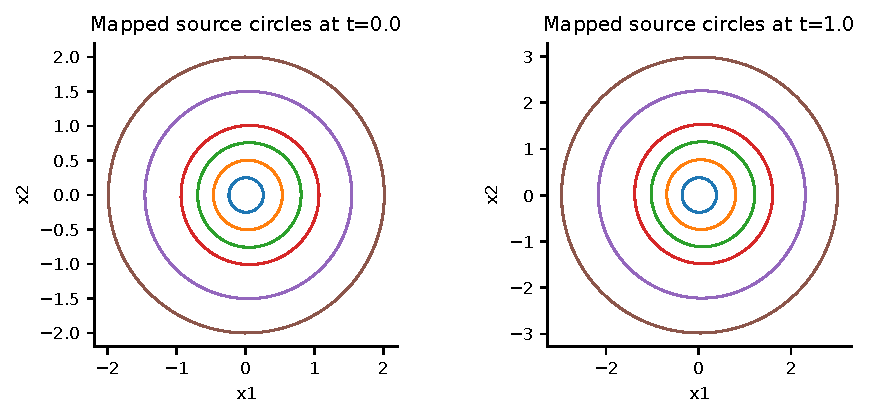
\includegraphics[width=0.85\linewidth]{../results/revision/harmonic_shape.pdf}
\caption{Images of concentric source circles under $F_0$ and $F_1$, showing the asymmetric deformation. These are mapped source contours, not claimed level sets of the target density.}
\end{figure}

Starting with $z_0=e^{-(1+i)at}x$, the inverse iteration is
\[
 z_{j+1}=e^{-(1+i)at}x-b e^{(1+i)a(\sqrt2-1)t}z_j^2e^{-|z_j|^2}.
\]
Its declared contraction factor is
$\rho_t=(4/e)b e^{a(\sqrt2-1)t}<0.313$.
We stop when $\rho_t\|z_{j+1}-z_j\|_\infty/(1-\rho_t)\le2\times10^{-14}$.
This is the exact-arithmetic contraction error bound evaluated in floating point, not a roundoff-inclusive enclosure. A refinement uses $2\times10^{-15}$. The main $N=512$ corrected-Euler run uses $8{,}319$ batch inverse iterations for $512$ field evaluations, about $16.25$ iterations per evaluation. Every solver stage, including every Heun and RK3 stage, pays this cost. No neural network, numerical score, numerical Jacobian, or Poisson solve is used in this example.

\subsection{An exact residual objective with an observable bad local minimum}
Set $n\in\{1,2\}$,
\[
 \zeta_n=a\sqrt n+i\{a\sqrt n+n(\omega-a)\},\qquad
 k_t(F_tz)=D F_t(z)Jz=\sum_{n=1}^2 inF_n(t,z).
\]
The acceleration along this gauge is $\sum_n\zeta_n^2F_n$.
The field $w_t=ck_t$ preserves $p_t$, so the following is an upper certificate for the weighted-gradient acceleration residual, not generally an equality with that projection norm:
\[
 R_t(\omega,c)^2
 =\|\mathbf a_\omega-ck_t\|_{L^2(p_t)}^2
 =\sum_{n=1}^2M_n(t)|\zeta_n^2-inc|^2,
\]
where
\[
 M_1(t)=2e^{2at},\qquad
 M_2(t)=\frac8{125}b^2e^{2a\sqrt2t}.
\]
The second identity follows from angular orthogonality and
$\mathbb E[|Z|^4e^{-2|Z|^2}]=8/125$.
Both masses increase, so $\sup_{0\le t\le1}R_t=R_1$ for fixed $(\omega,c)$.
Eliminating $c$ gives
\[
 c_*(\omega)=\frac{\sum_n nM_n(1)\operatorname{Im}(\zeta_n^2)}
                  {\sum_n n^2M_n(1)}.
\]
The remaining objective is a coercive quartic. The code enumerates all real roots of its cubic derivative, then compares objective values using the original sum of squares. Its three stationary points have $\omega$ approximately $-0.392394$, $0.000331763$, and $0.4$. Their residuals are approximately $0.0724104$, $0.3388934$, and floating-point zero. The first and third are local minima; the middle is a local maximum. Local least squares from $(\omega,c)=(-0.3,0)$ terminates at the inferior minimum. Starts $(0.07,0.03)$ and $(0.8,-0.2)$ reach the zero. The optimizer is therefore not treated as a global feasibility certificate; the finite stationary-point enumeration and the exact coefficient argument supply that distinction.

\begin{figure}[htbp]
\centering
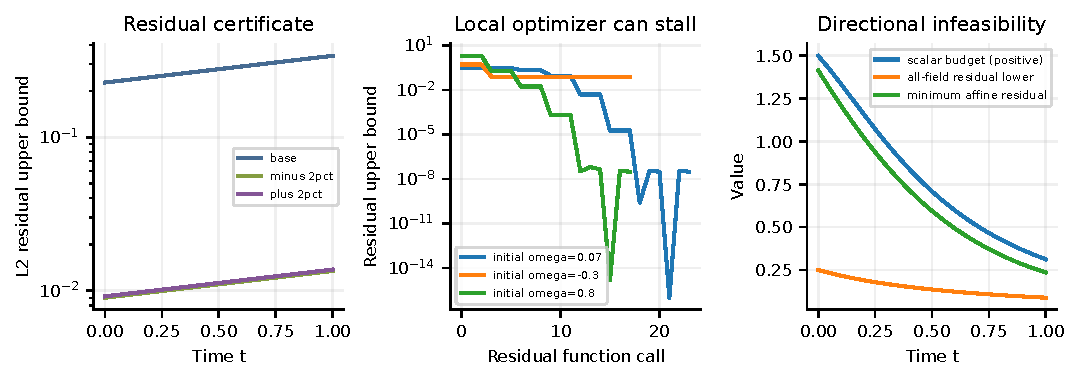
\includegraphics[width=\linewidth]{../results/revision/residual_discovery.pdf}
\caption{Left: exact formulas for residual upper certificates. The discovered solution is omitted from this logarithmic panel because its exact residual is zero. Center: local optimization from three initial values; the negative start stagnates at a positive residual. Right: the directional obstruction for a Gaussian path whose scalar energy budget is positive. The affine residual curve uses the global minimum of its even quartic objective.}
\end{figure}

\subsection{Distribution bounds and quadrature refinement}
For a numerical endpoint $\widehat X_N(Z)$, the lower bound is
\[
 \left|\sqrt{\mathbb E|\widehat X_N|^2}
       -\sqrt{M_1(T)+M_2(T)}\right|\le W_2(\widehat p_N,p_T).
\]
For corrected Euler, the upper bound uses the valid target coupling
$F_T(e^{-ia^2Th}Z)$, with $h=T/N$, as proved in Theorem~\ref{thm:harmonic-coupling}. For a perturbed $\omega$, we use
$F_T(e^{i\{(\omega-a)T-c_*(\omega)Th/2\}}Z)$.
Every such fixed rotation preserves the Gaussian source, so the pairing remains a valid upper bound even when no second-order guarantee is claimed. For base Euler, Heun, and RK3, the same-start coupling is used. We do not minimize these couplings or identify their RMS with full $W_2$.

The radial rule uses $s=|Z|^2/2\sim\operatorname{Exp}(1)$, with positive Gauss--Laguerre weights; the angular rule uses equally spaced points on $[0,2\pi)$. The main rule has $64\times64=4{,}096$ nodes. Refining to $96\times128=12{,}288$ nodes changes the $N=512$ corrected upper estimate by $7.8\times10^{-17}$ and the base upper estimate by less than $7\times10^{-15}$. The corrected lower estimate is unchanged at printed double precision. Tightening inverse tolerance by a factor ten changes the corrected upper estimate by less than $4\times10^{-18}$. A coarser $32\times32$ rule changes the corrected lower bound by about $3.1\times10^{-11}$; the fine rule is used throughout. This is a refinement study, not a rigorous quadrature error enclosure.

An independent DOP853 solve uses relative tolerance $2\times10^{-12}$ and absolute tolerance $2\times10^{-13}$ on five fixed labels, for the base, discovered, and $-2\%$-perturbed fields. Four observation times $1/4,1/2,3/4,1$ give a maximum discrepancy of $6.5\times10^{-12}$ from the analytic trajectories. Tests also compare acceleration with a second time difference of the exact nonlinear trajectory, so omission of the nonlinear-coordinate Hessian term would be detected.

\subsection{A path that passes the scalar budget but is infeasible}
Let $\Sigma_t=\operatorname{diag}(1+t,1+t+2t^2)$ and $p_t=\mathcal N(0,\Sigma_t)$. The gradient field is
$v_t=\frac12\dot\Sigma_t\Sigma_t^{-1}x$.
The scalar budget $\frac12(\operatorname{tr}\Sigma_t)''-\mathbb E|v_t|^2$ remains at least $0.3125$ over $[0,1]$. Nevertheless, $m_1(t)=\mathbb E X_1^2=1+t$ has zero second derivative and nonzero first derivative. Every admissible velocity satisfies
\[
 \mathbb E[u_1^2]\ge\frac1{4(1+t)},\qquad
 \mathbb E[X_1a_1]=-\mathbb E[u_1^2],\qquad
 \|P_{p_t}^{\nabla}\mathbf a_t\|_{L^2(p_t)}
 \ge\frac1{4(1+t)^{3/2}}.
\]
This is an all-field obstruction under the stated moment and integration-by-parts assumptions, not a failure of one optimizer.
As a diagnostic comparison, the code minimizes over all two-dimensional affine Gaussian gauges $A=v+\omega\Sigma^{1/2}J\Sigma^{-1/2}$. The acceleration's weighted-gradient projection is $Sx$, where
\[
 S\Sigma+\Sigma S=\ddot\Sigma-2A\Sigma A^\top,\qquad
 \varepsilon^2=\operatorname{tr}(S\Sigma S).
\]
This objective is an even quartic in $\omega$, so its global minimum follows from a quadratic minimization in $\omega^2\ge0$. The affine curve in the figure does not assert that every admissible non-affine field has the same minimum.

\subsection{A learned coefficient and a continuous-path error floor}
To separate learned-path error from integration error, define the restricted regression family
\[
 u_{\delta,\omega}(t,F_tz)
 =\partial_tF_tz+\delta D F_t(z)z+(\omega-a)D F_t(z)Jz.
\]
Its exact trajectory is $F_t(e^{\delta t}e^{i(\omega-a)t}z)$.
We observe $512$ independent pairs $(t,z)$, with $t$ uniform on $[0,1]$ and $z$ standard planar Gaussian, and noisy base velocities $v(t,F_tz)+\xi$, where the two coordinates of $\xi$ are independent $\mathcal N(0,0.08^2)$. Ordinary one-parameter least squares fits the coefficient of $D F_t(z)z$ around the specified base field. The true coefficient is zero; it is not supplied to the fit. Seeds $7,19,42$ give fitted coefficients approximately $-0.00060835$, $-0.00031947$, and $0.00253611$, respectively. Their known-noise standard errors are about $0.0020$. This experiment tests one identifiable coefficient with an exact model, not general neural velocity learning.

After adding the gauge $\omega=a$, the learned path is $p_t^\delta=(F_t\circ e^{\delta t})_\#\rho$. Its second moment is known exactly:
\[
 \mathbb E_{p_t^\delta}|X|^2
 =2e^{2at}s^2
  +b^2e^{2a\sqrt2t}\frac{8s^4}{(1+4s^2)^3},\qquad s=e^{\delta t}.
\]
We bound $W_2(p_T^\delta,p_T)$ below by the second-moment discrepancy and above by the common-label RMS between $F_T(e^{\delta T}Z)$ and $F_T(Z)$. These bounds give path-error intervals approximately
$[0.0012814,0.0012850]$,
$[0.0006730,0.0006749]$, and
$[0.0053504,0.0053654]$ for the three seeds.
At $N=512$, numerical-to-learned-path coupling upper bounds are between $8.9\times10^{-7}$ and $6.0\times10^{-6}$, while numerical-to-target error remains near these much larger path-error floors. The approximate fields are not claimed to satisfy exact acceleration preservation.

\begin{figure}[htbp]
\centering
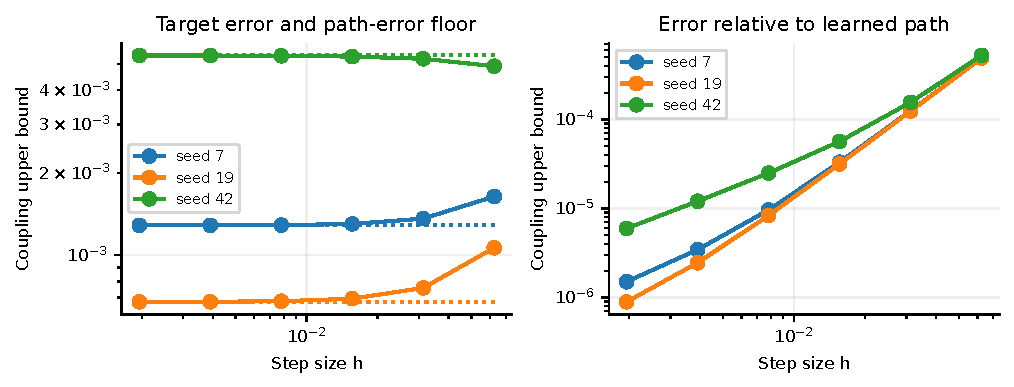
\includegraphics[width=\linewidth]{../results/revision/learned_path_floor.pdf}
\caption{Restricted learned-field experiment. Dotted lines are continuous-path coupling upper bounds. Integration refinement reduces error relative to the learned path but cannot remove error in the learned continuous distribution. Curves and floors are quadrature evaluations of valid upper couplings; they are not exact $W_2$ evaluations.}
\end{figure}

\subsection{Runtime, reproducibility, and limitations}
Equal-cost runs use budgets $48,96,192,384$ field evaluations; Euler uses $N$ steps, Heun $N/2$, and RK3 $N/3$. Each batch contains $4{,}096$ deterministic quadrature labels. Timings are the median of three repetitions, with minima and maxima retained in \texttt{equal\_cost.csv}. At $384$ evaluations, batch times are of the same order (a few tenths of a second) for all three methods. The correction search, including unsuccessful local searches, takes about $0.01$ seconds. The one-coefficient regression solve takes about $10^{-5}$ seconds after generating the data. These are CPU implementation measurements; they neither predict neural-network evaluation costs nor establish an end-to-end generation speedup. The observed Heun advantage is small, so we retain bounds and numerical refinement data rather than interpreting wall-clock differences of this size as significant. RK3's accuracy advantage is much larger.

\begin{figure}[htbp]
\centering
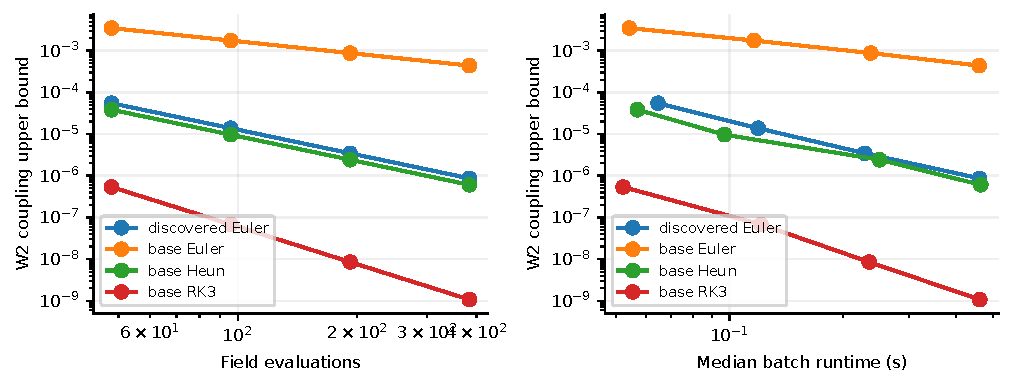
\includegraphics[width=\linewidth]{../results/revision/harmonic_cost.pdf}
\caption{Coupling upper bounds versus field-evaluation count and measured median batch runtime. The different methods use different couplings, so upper-bound curves alone do not order exact Wasserstein errors; Table~\ref{tab:revision-cost} also reports lower bounds.}
\end{figure}

The recorded environment is Linux x86\_64, Python 3.12.14, NumPy 2.3.5, and SciPy 1.17.0. The CPU reports Intel Xeon Platinum 8573C. We set \texttt{OMP\_NUM\_THREADS}, \texttt{OPENBLAS\_NUM\_THREADS}, and \texttt{MKL\_NUM\_THREADS} to one. The code does not claim a measured peak-memory advantage; it uses vectorized arrays of batch size $4{,}096$, and the exact small optimization eliminates any neural-training storage in this example.
Run
\begin{verbatim}
OMP_NUM_THREADS=1 OPENBLAS_NUM_THREADS=1 \
MKL_NUM_THREADS=1 python3 -B scripts/run_revision.py
python3 -B -m unittest discover -s tests -v
\end{verbatim}
from the repository root after installing the declared dependencies. The first command regenerates raw CSV files, the machine-readable summary, the table, and five figures under \texttt{results/revision/}. The original reproduction command regenerates the pre-existing Gaussian, nonlinear radial, and solver-comparison results separately. All $63$ original tests and $9$ new independent tests pass. The original reproduction regenerated $81$ baseline runs and $33$ nonlinear runs with $16{,}983$ and $24{,}600$ node comparisons, respectively; the original manuscript's rounded numerical macros agree exactly. No image-generation benchmark, high-dimensional learned model, or universal correction algorithm is claimed.

% Detailed established results, retained from the original preprint.
\section{Error measures and the acceleration condition}
\label{sec:setup}

\begin{center}
\small
\begin{tabular}{@{}p{0.22\linewidth}p{0.57\linewidth}p{0.14\linewidth}@{}}
\toprule
Term or symbol & Meaning & Definition\\
\midrule
Probability path $p_t$ & The distribution specified at each time $t$ & Section~\ref{sec:path}\\
Local and global error & Error from one Euler step started from the exact distribution, and error accumulated through repeated steps & Section~\ref{sec:path}\\
Particle error & Root mean squared distance using the same starting point & Section~\ref{sec:errors}\\
Coupling and $W_2$ & A joint distribution with given marginals, and the least root mean squared distance over all such pairings & Eq.~\eqref{eq:w2}\\
Material acceleration $\acc_t$ & Velocity change along an exact particle & Eq.~\eqref{eq:acceleration}\\
Acceleration condition & $\int\nabla\phi\cdot\acc_t\,\dd p_t=0$ for every smooth compactly supported $\phi$ and every $t$ & Definition~\ref{def:flux}\\
Kinetic action $\cA_T$ & Time integral of kinetic energy $\E_{p_t}\|u_t\|^2$ & Eq.~\eqref{eq:action}\\
Second moment $M(t)$ & $\E_{p_t}\|X\|^2$ & Section~\ref{sec:path-restrictions}\\
\bottomrule
\end{tabular}
\end{center}

\subsection{The probability path and Euler's method}
\label{sec:path}

A velocity field $u$ generates the probability path $(p_t)_{0\le t\le T}$ when the solution of $\dot X_t=u(t,X_t)$, with $X_0\sim p_0$, has distribution $p_t$ at each time. Each $p_t$, called a \emph{marginal distribution}, describes positions at one time without recording the particles' starting points. Different particle motions can therefore give the same probability path, as the outward and rotating Gaussian fields do. We assume finite second moments and write $\E$ for expectation, $\Law$ for distribution, and $\|\cdot\|$ for the Euclidean norm. Single bars $|\cdot|$ denote scalar absolute value or complex modulus, while $\|\cdot\|_{\rm op}$ denotes the induced operator norm of a linear or multilinear map.

On a grid $0=t_0<\cdots<t_N=T$, with step lengths $h_k=t_{k+1}-t_k$ and largest step $H=\max_kh_k$, Euler's method is
\begin{equation}
 \widehat X_{k+1}=\widehat X_k+h_ku(t_k,\widehat X_k),
 \qquad \widehat X_0\sim p_0,\qquad
 \widehat p_k=\Law(\widehat X_k).
 \label{eq:euler}
\end{equation}
For $u(x)=x$, a particle starting at one reaches $1.1$ after an Euler step of length $0.1$ and reaches $1.21$ after the next step. The second step starts from the first numerical position, so it includes the error from the first step. We call the error after repeated steps the \emph{global error}. The \emph{local error} is the error from one step that starts from the exact distribution $p_t$. We compare fields on the same grid. When studying convergence, we decrease the step sizes while keeping both fields and the final time fixed.

\subsection{Particle error and distribution error}
\label{sec:errors}

A rotation shows why particle displacement and distribution change can differ. Rotating the uniform unit circle by $30^\circ$ moves each point by $2\sin(15^\circ)\approx0.518$, although the distribution stays the same. We can pair each rotated point with an original point at the same location, giving zero distance between the distributions. Such a pairing is a \emph{coupling}, a joint distribution with the two given marginal distributions. The Wasserstein distance is the least root mean squared distance over these couplings,
\begin{equation}
 W_2(\mu,\nu)=
 \left(\inf_{\gamma\in\Gamma(\mu,\nu)}
 \int\|x-y\|^2\dd\gamma(x,y)\right)^{1/2},
 \label{eq:w2}
\end{equation}
where $\Gamma(\mu,\nu)$ is the set of couplings of $\mu$ and $\nu$. Particle error uses the numerical and exact particles from the same starting point. Its root mean squared value is $\|\widehat X_N-X_T\|_{L^2}=(\E\|\widehat X_N-X_T\|^2)^{1/2}$. This pairing is one of the couplings in Eq.~\eqref{eq:w2}, so distribution error cannot exceed particle error. Practical sampling metrics also compare distributions. For example, Fr\'echet Inception Distance uses the squared Wasserstein distance between Gaussian fits to feature distributions~\citep{heusel2017gans}. Our examples use $W_2$ between the full distributions.

We calculate the errors from Gaussian formulas or deterministic quadrature, so they have no sampling uncertainty. Smaller values mean better accuracy in all figures and tables. An $O(H^2)$ bound means that the error is at most a constant times $H^2$ for small $H$, but the error could decrease faster. A positive limit of error divided by $h^2$ shows that second order is the actual rate. In that case, halving a sufficiently small uniform step reduces the error by approximately a factor of four.

\subsection{The acceleration condition}
\label{sec:condition}

For a density $p_t$, the continuity equation $\partial_t p_t+\nabla\cdot(p_tu_t)=0$ describes how the velocity field changes the distribution. Adding a field $r_t$ with $\nabla\cdot(p_tr_t)=0$ leaves this equation unchanged, although it can change how individual particles move. When the probability measure has no density, we express the same condition using expectations of smooth functions. We apply it to material acceleration and use \emph{jerk} for the change in acceleration along an exact trajectory,
\begin{equation}
 \acc_t=\partial_tu_t+(D_xu_t)u_t,\qquad
 \jerk_t=\partial_t\acc_t+(D_x\acc_t)u_t.
 \label{eq:acceleration}
\end{equation}
Here $\acc_t(X_t)$ and $\jerk_t(X_t)$ are the second and third time derivatives of the exact particle position. The term $(D_xu_t)u_t$ accounts for the change in velocity caused by the particle's motion through space.

\begin{definition}[Distribution-preserving fields and the acceleration condition]
\label{def:flux}
A field $w$ has \emph{zero weighted divergence under} a probability measure $p$ if
\begin{equation}
 \int \nabla\phi(x)\cdot w(x)\,p(\dd x)=0
 \quad\text{for every }\phi\in C_c^\infty(\R^d),
 \label{eq:flux-null}
\end{equation}
where the tests are smooth and compactly supported. A velocity field $u$ satisfies the \emph{acceleration condition} along $(p_t)$ if Eq.~\eqref{eq:flux-null} holds with $w=\acc_t$ and $p=p_t$ at every time.
\end{definition}

Zero weighted divergence refers to the probability measure $p$, while ordinary zero divergence refers to volume. For example, rotation preserves a circularly symmetric distribution because it keeps the angle uniform. A constant rightward field also has zero ordinary divergence, but it moves a Gaussian to the right and changes its distribution. Under the regularity assumptions of Proposition~\ref{prop:frozen-preservation}, Eq.~\eqref{eq:flux-null} means that the flow of $w$ preserves $p$ exactly. For acceleration, this means that motion along $\acc_t$ preserves $p_t$ while physical time $t$ is held fixed.

\subsection{Kinetic action as a comparison objective}

Penalties on speed or velocity derivatives are used to make numerical integration easier~\citep{finlay2020regularization,kelly2020easy,lee2023curvature}. We compare Euler's distribution error with kinetic action, the time integral of average squared speed,
\begin{equation}
 \cA_T(u)=\int_0^T\E_{p_t}\|u(t,X)\|^2\dd t,
 \label{eq:action}
\end{equation}
where the integrand is kinetic energy, defined here without the factor $1/2$. The base fields in Sections~\ref{sec:gaussian} and~\ref{sec:nonlinear} minimize this action among finite-action fields that satisfy the same weak continuity equation. Their Euler distribution errors are nevertheless larger than those of the corrected fields. Section~\ref{sec:path-restrictions} proves this action comparison and shows which restrictions the acceleration condition places on the path.


\section{Rotation separates the two error orders for a Gaussian}
\label{sec:gaussian}

For a Gaussian path, we can find the correction by comparing how Euler and the exact flow change the radius. Let $J$ be a quarter-turn in two dimensions, so $Jx$ is perpendicular to $x$ and has the same length. The field $ax+bJx$ combines expansion at rate $a>0$ with rotation at rate $b$. An Euler step sends $x$ to $(1+ah)x+bhJx$ and multiplies the squared radius by $(1+ah)^2+b^2h^2$. The exact expansion gives $e^{2ah}=1+2ah+2a^2h^2+O(h^3)$, while Euler without rotation misses one $a^2h^2$ term. Choosing $b=a$ supplies this term, and the same choice works as the step size changes.

For the probability path
\begin{equation}
 p_t=\mathcal N(0,e^{2at}I_2),\qquad a>0,
 \label{eq:gaussian-path}
\end{equation}
the base and corrected fields are therefore
\begin{equation}
 v_0(x)=ax,\qquad v_1(x)=a(I+J)x.
 \label{eq:fixed-fields}
\end{equation}
These fields are part of the known Gaussian rotation family~\citep{lim2025hidden}. We use them to compare action, distribution error, and particle error. A linear change of coordinates gives the same construction for every positive definite covariance in even dimension. Euler also reproduces an added affine mean exactly. Appendix~\ref{app:fixed-gaussian} gives these extensions, and Figure~\ref{fig:gaussian} shows an elliptical Gaussian example.

\begin{theorem}[Gaussian distribution and particle errors]
\label{thm:fixed-gaussian}
For the fields in Eq.~\eqref{eq:fixed-fields} on $[0,T]$ with $T>0$, the base field $v_0$ minimizes kinetic action among finite-action fields satisfying the same weak continuity equation. The corrected field adds $a(e^{2aT}-1)>0$ to that action. Euler's numerical covariance is $q_{i,k}I_2$, where
\begin{equation}
 q_{0,k}=\prod_{j<k}(1+ah_j)^2,\qquad
 q_{1,k}=\prod_{j<k}(1+2ah_j+2a^2h_j^2).
 \label{eq:fixed-covariance}
\end{equation}
At every grid point after the start,
\begin{equation}
 0<W_2(\widehat p_k^1,p_{t_k})
   <W_2(\widehat p_k^0,p_{t_k}),\qquad
 W_2(\widehat p_k^i,p_{t_k})
 =\sqrt{2}\,[e^{at_k}-\sqrt{q_{i,k}}].
 \label{eq:fixed-error}
\end{equation}
For uniform $h=T/N\to0$, write $C_\Sigma=\sqrt{2}e^{aT}$. Then
\begin{align}
 W_2(\widehat p_N^0,p_T)&=C_\Sigma\,\tfrac12a^2T h+O(h^2),
 \label{eq:base-order}\\
 W_2(\widehat p_N^1,p_T)&=C_\Sigma\,\tfrac23a^3T h^2+O(h^3),
 \label{eq:fixed-order}\\
 \|\widehat X_N^1-X_T^1\|_{L^2}
 &=C_\Sigma\,a^2T h+O(h^2).
 \label{eq:particle-order}
\end{align}
\end{theorem}

For $z=ah>0$, the covariance factors satisfy $(1+z)^2<1+2z+2z^2<e^{2z}$. Both numerical clouds are therefore too small, but the corrected cloud is closer to the exact size. Multiplying these factors keeps the same strict ordering on every increasing grid. To find the error orders, we take logarithms and add the errors over the steps. The one-step log-scale errors are $z-\log(1+z)=z^2/2+O(z^3)$ for the base field and $z-\frac12\log(1+2z+2z^2)=2z^3/3+O(z^4)$ for the corrected field. On a uniform grid, the sum over $T/h$ steps gives first-order and second-order errors, respectively.


An optimal coupling pairs Gaussian points at the same angle, so the distribution error depends only on scale. Particle error also includes the angle error between particles from the same starting point. The base field has no angle error. Eqs.~\eqref{eq:base-order} and~\eqref{eq:particle-order} show that adding the correction doubles the leading particle error coefficient, although distribution error becomes second order. The elliptical Gaussian in Figure~\ref{fig:gaussian} has the same behavior. Increasing the uniform step count from 32 to 64 reduces base distribution error from $1.51\times10^{-2}$ to $7.63\times10^{-3}$, a factor of $1.98$. Corrected distribution error decreases from $3.74\times10^{-4}$ to $9.47\times10^{-5}$, a factor of $3.94$. Appendix~\ref{app:fixed-gaussian} gives the proof and bounds for unequal steps.

\begin{figure}[t]
\centering
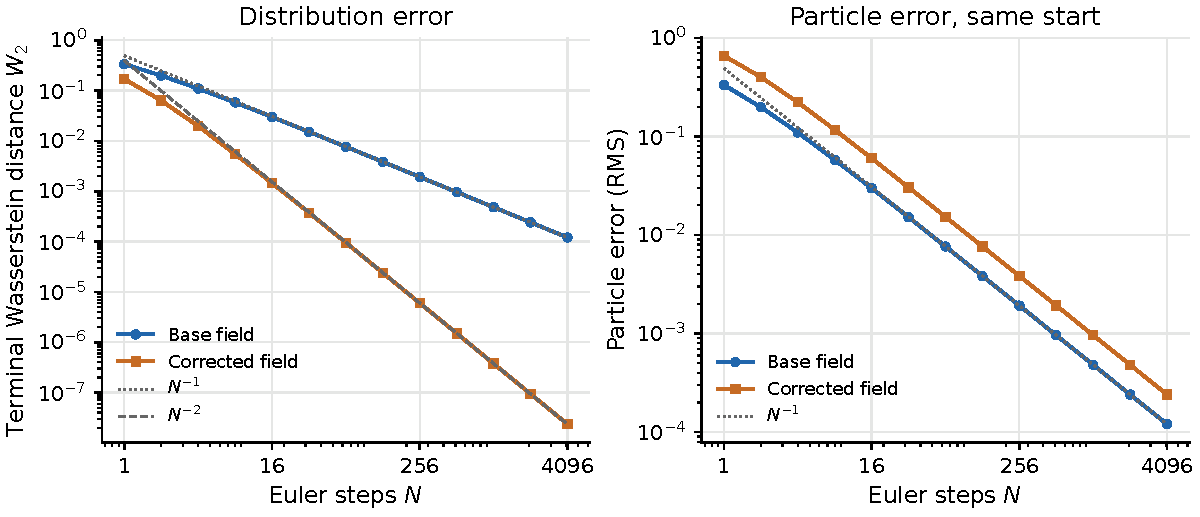
\includegraphics[width=\linewidth]{../results/gaussian_convergence.pdf}
\caption{Adding rotation gives second-order Gaussian distribution error, although particle error remains first order with twice the base field's leading coefficient. The left panel shows $W_2$ between numerical and exact distributions. The right panel shows particle error from the same starting point. The fields stay fixed as the uniform step count $N$ increases, and the reference lines show the $N^{-1}$ and $N^{-2}$ rates. Parameters are $a=0.6$, $T=1$, and $\Sigma_0=\left(\begin{smallmatrix}1.5&0.25\\0.25&0.75\end{smallmatrix}\right)$.}
\label{fig:gaussian}
\end{figure}


This improvement on every grid requires expansion. During contraction, the added rotation can make the numerical radius too large. For $a=-0.6$ and one step of length one, the base scale $0.4$ is closer to the exact scale $e^{-0.6}\approx0.549$ than the corrected scale $\sqrt{0.52}\approx0.721$.

For the expanding circular Gaussian, the corrected acceleration is $2a^2Jx$. Motion along this field follows circles and preserves the distribution. We use the same property below to bound the error without assuming a Gaussian path.


\section{The acceleration condition bounds global distribution error}
\label{sec:general}

A velocity field can preserve a distribution even when its acceleration does not. For steady rotation $u(x)=Jx$ on the uniform unit circle, the velocity preserves the distribution, but the acceleration $\acc(x)=J^2x=-x$ points inward. Motion along this acceleration shrinks the circle. The corrected expanding Gaussian has tangential acceleration, so motion along its acceleration preserves the distribution. This is the property we use to bound Euler's distribution error.

\subsection{A coupling that reduces the local error}

Let $E_{t,h}(x)=x+hu_t(x)$ be the Euler map and $F_{t,t+h}$ the exact flow over the same interval. Hold physical time $t$ fixed, and let $\Psi_t^\tau$ be the flow that follows $\acc_t$ for duration $\tau$. Under the acceleration condition and the regularity assumptions below, $X\sim p_t$ and $\Psi_t^\tau X$ have the same distribution. Applying Euler to either starting point therefore gives the same output distribution. We can use the shifted start for Euler and the original start for exact motion to form a closer pairing.

The choice $\tau=h^2/2$ supplies the leading displacement that Euler omits. We write $O_{L^2}(h^q)$ for a remainder whose root mean squared norm is at most $Ch^q$, with $C$ independent of $h$ as $h\downarrow0$. The shifted start satisfies $\Psi_t^{h^2/2}X=X+h^2\acc_t(X)/2+O_{L^2}(h^4)$. Evaluating velocity at this point changes the Euler displacement by only $O_{L^2}(h^3)$. Thus the root mean squared distance between $E_{t,h}(\Psi_t^{h^2/2}X)$ and $F_{t,t+h}(X)$ is $O(h^3)$, as Figure~\ref{fig:coupling} shows. For the circular Gaussian with $a=0.6$, the shift rotates the start by $2a^2\tau=0.36h^2$.

\begin{figure}[htbp]
\centering
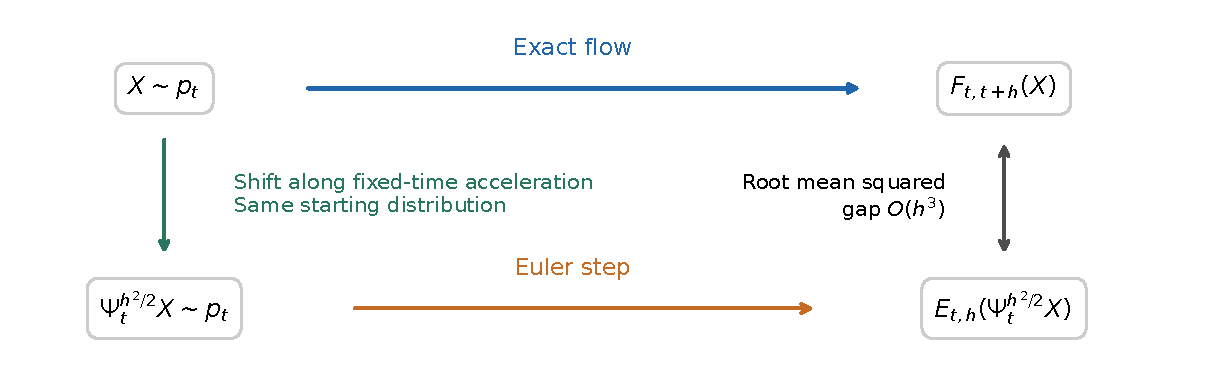
\includegraphics[width=\linewidth]{../results/figures/acceleration_coupling.pdf}
\caption{Shifting the start along the acceleration field gives a closer pairing and keeps Euler's output distribution unchanged. During the shift, physical time is held fixed and the distribution remains $p_t$. The shift supplies the leading displacement that Euler omits. We pair the Euler output from the shifted start with exact motion from the original start. Under Theorem~\ref{thm:distribution_order}, their root mean squared distance is $O(h^3)$.}
\label{fig:coupling}
\end{figure}
\FloatBarrier

To obtain the global bound, we also need to control how later steps increase this local error. Two continuous derivatives of velocity give the trajectory expansion. Global Lipschitz bounds control how far apart the outputs can be when the inputs differ, and mean square bounds allow us to integrate over the distribution. The theorem states these assumptions.

The exact theorem statement is Theorem~\ref{thm:distribution_order} in the main paper.


Each step adds an error bounded by a constant times $h_j^3$. The sum $\sum_j h_j^3\le TH^2$ gives the total contribution of these errors, and $e^{LT}$ bounds how much later Euler steps can increase them. The error is therefore at most a constant times $H^2$ at every grid point, without any Gaussian or symmetry assumption. The theorem gives a test for a particular field. It does not give a suitable field for every path, and Section~\ref{sec:path-restrictions} shows that some paths cannot satisfy the condition. Appendix~\ref{app:general} proves the bound using the local coupling and the Euler stability estimate $1+Lh$.

\subsection{Local necessity and weak error}

The acceleration condition is also necessary if one Euler step from the exact distribution has error $o(h^2)$. Here $o(h^2)$ means that the error divided by $h^2$ tends to zero. For this rate to hold, the acceleration must preserve the distribution in the sense of Eq.~\eqref{eq:flux-null}.
\begin{proposition}[Local converse]
\label{prop:local-converse}
Let $u$ and $p_t$ satisfy the regularity, growth, and moment assumptions of Theorem~\ref{thm:distribution_order}, without imposing the acceleration condition. At a fixed $t<T$, suppose
\[
 W_2((E_{t,h})_\#p_t,p_{t+h})=o(h^2)
 \quad\text{as }h\downarrow0.
\]
Then $\acc_t$ satisfies Eq.~\eqref{eq:flux-null} under $p_t$.
\end{proposition}
Here $(E_{t,h})_\#p_t$ is the distribution obtained by applying Euler to a point drawn from $p_t$. The result concerns one step from the exact distribution. Errors across several steps can cancel at the final time, even when the acceleration condition fails. For example, the field $u(t,x)=\sin(2\pi t)e_1$ on $[0,1]$ with a Gaussian source has zero exact displacement and zero total Euler displacement on every uniform grid. Euler therefore gives the exact terminal distribution, although the acceleration changes the current distribution whenever it is nonzero. Appendix~\ref{app:local} gives the proof and this example.

For a smooth compactly supported test function $\phi$, the difference between expectations after one Euler step and exact motion is
\begin{equation}
 \E_{p_t}\phi(E_{t,h}X)-\E_{p_{t+h}}\phi
 =-\tfrac12h^2\int\nabla\phi\cdot\acc_t\,\dd p_t+o(h^2).
 \label{eq:weak-defect}
\end{equation}
Under the proposition's assumptions, the absolute difference in expectations is at most the Lipschitz constant of $\phi$ times $W_2$. If $W_2=o(h^2)$, the leading integral in Eq.~\eqref{eq:weak-defect} must therefore be zero. This gives the acceleration condition. Appendix~\ref{app:local} justifies the remainder, and Proposition~\ref{prop:weak-euler} in Appendix~\ref{app:weak} gives an explicit cubic bound under a stronger moment assumption. Earlier global weak expansions follow expectation errors through the later exact flow~\citep{talay1990expansion,hurault2026geometry}. The coupling in Theorem~\ref{thm:distribution_order} bounds the distribution distance directly.

\section{A nonlinear path has different error orders}
\label{sec:nonlinear}

The same difference in error orders is possible when the distribution changes shape. We use a radial distribution whose outer radii expand by larger relative factors. Unlike uniform expansion, this motion does not multiply all radii by the same number. Radial symmetry still gives an optimal pairing by radius, so we can compare errors when a covariance calculation is no longer enough.

We choose the rotation to cancel the radial part of acceleration. For the outward field $\alpha(r)x$, this part is $[\alpha(r)^2+\alpha(r)r\alpha'(r)]x$. Adding the tangential velocity $\beta(r)Jx$ contributes $-\beta(r)^2x$ to the radial acceleration. Choosing $\beta(r)^2=\alpha(r)^2+\alpha(r)r\alpha'(r)$ cancels the radial acceleration. The remaining tangential acceleration preserves a radial distribution. We choose an increasing $\alpha$ so that the relative expansion depends on radius. We also keep $\alpha$ bounded to control growth at large radii. With $J=\left(\begin{smallmatrix}0&-1\\1&0\end{smallmatrix}\right)$ and $a,\eta>0$, define
\begin{equation}
 \alpha(r)=a+\eta\frac{r^2}{1+r^2},\qquad
 P(r)=\alpha(r)^2+\alpha(r)r\alpha'(r),\qquad
 \beta(r)=\sqrt{P(r)}.
 \label{eq:nonlinear-coefficients}
\end{equation}
The positive function $P$ gives a real rotation rate, and the resulting base and corrected fields are
\begin{equation}
 u_0(x)=\alpha(\|x\|)x,\qquad
 u_1(x)=\alpha(\|x\|)x+\beta(\|x\|)Jx.
 \label{eq:nonlinear-fields}
\end{equation}

For both fields, the radius satisfies $\dot R=\alpha(R)R$. We write $R(t,r)$ for its solution from radius $r$, with $R(0,r)=r$. When the source is rotationally invariant, the added rotation keeps the angle uniform at each positive radius and leaves the origin fixed. The two fields therefore give the same distribution at every time, although their particles follow different trajectories. Since $\alpha$ increases with radius, the distribution changes shape whenever the source support contains two distinct positive radii.

For example, $a=0.6$ and $\eta=0.3$ give relative expansion rates $\alpha(1)=0.75$ and $\alpha(2)=0.84$. The outer circle therefore grows faster relative to its own radius. Figure~\ref{fig:shape} shows this shape change by dividing radius quantiles by the median radius. These ratios change along the nonlinear path. They would stay constant if every radius grew by the same factor.

\begin{figure}[ht]
\centering
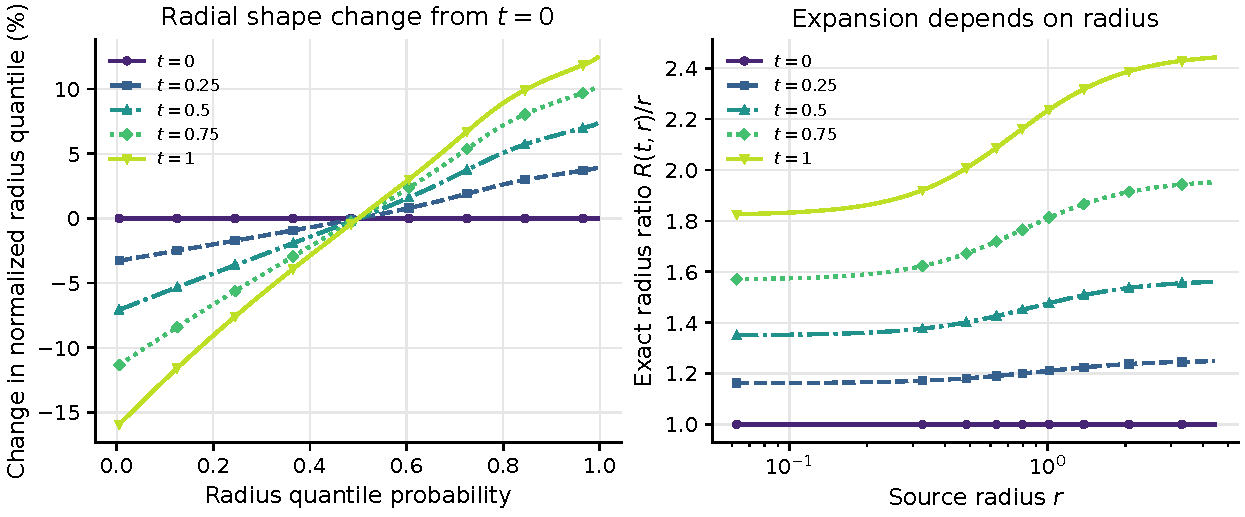
\includegraphics[width=\linewidth]{../results/figures/nonlinear_shape.pdf}
\caption{The nonlinear distribution changes shape because outer radii expand by larger relative factors. The left panel shows the percentage change, from $t=0$, in each radius quantile divided by the median radius. Uniform scaling would leave these ratios unchanged. The right panel shows the expansion factor as a function of starting radius, with the parameters of Figure~\ref{fig:nonlinear}.}
\label{fig:shape}
\end{figure}

The corrected field also satisfies the acceleration condition. Differentiation gives
\begin{equation}
 \acc_{u_1}(x)=\beta_a(\|x\|)Jx,\qquad
 \beta_a(r)=2\alpha(r)\beta(r)+\alpha(r)r\beta'(r)\ge2a^2.
 \label{eq:nonlinear-acceleration}
\end{equation}

This acceleration is tangent to each circle, so motion along it at fixed physical time preserves every radial distribution. The acceleration is nonzero away from the origin, so these trajectories are not straight with constant velocity as in Proposition~\ref{prop:gradient-straight}. The next theorem shows that the correction gives smaller distribution error on every grid. It also gives the exact error orders on uniform grids. Appendix~\ref{app:nonlinear} contains the regularity checks and proofs.

\begin{theorem}[Nonlinear error separation on every grid]
\label{thm:nonlinear}
Let $a,\eta,T>0$, and let $p_0$ be rotationally invariant on $\R^2$, with
$0<\E\|X_0\|^2<\infty$. The fields in Eq.~\eqref{eq:nonlinear-fields} are smooth and globally Lipschitz. They generate the same probability path. The base field minimizes kinetic action among finite-action fields satisfying the same weak continuity equation, and the correction strictly increases it. On every finite increasing time grid,
\begin{equation}
 0<W_2(\widehat p_k^1,p_{t_k})
   <W_2(\widehat p_k^0,p_{t_k})\qquad(k\ge1).
 \label{eq:nonlinear-ordering}
\end{equation}
On uniform grids $h=T/N\to0$, there are finite, strictly positive constants $\kappa_0,\kappa_1,\kappa_{\rm p}$ such that
\begin{equation}
 \frac{W_2(\widehat p_N^0,p_T)}{h}\to \kappa_0,\qquad
 \frac{W_2(\widehat p_N^1,p_T)}{h^2}\to \kappa_1,\qquad
 \frac{\|\widehat X_N^1-X_T^1\|_{L^2}}{h}\to \kappa_{\rm p}.
 \label{eq:nonlinear-limits}
\end{equation}
\end{theorem}

\begin{figure}[ht]
\centering
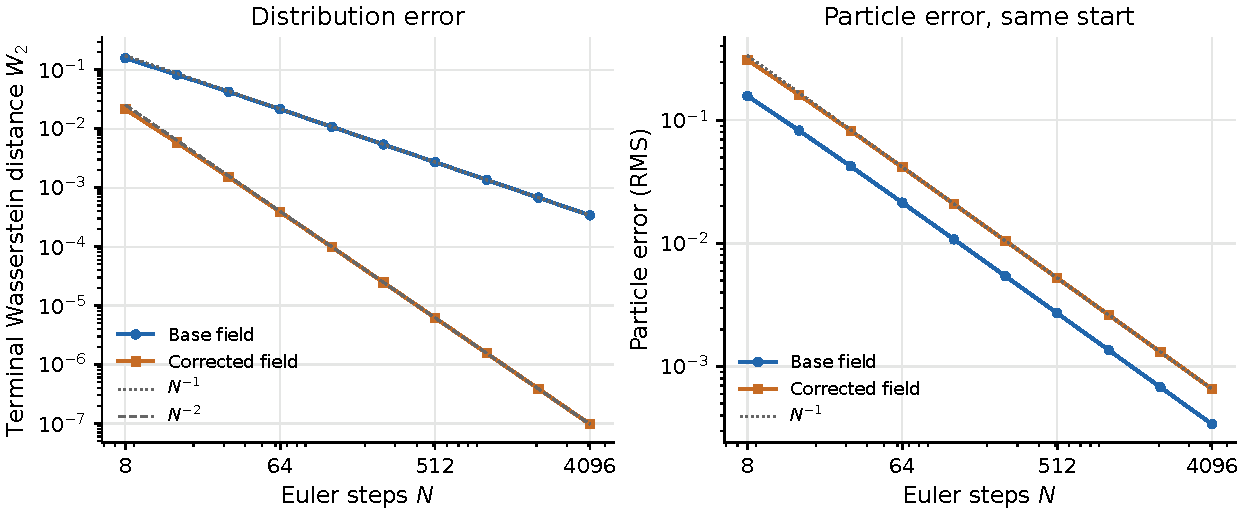
\includegraphics[width=\linewidth]{../results/figures/nonlinear_convergence.pdf}
\caption{The corrected nonlinear field gives second-order distribution error, although particle error remains first order with a larger leading coefficient. The left panel uses Eq.~\eqref{eq:radial-transport} to measure distribution error, while the right panel compares particles from the same start. Both fields remain fixed as the uniform step size decreases, and the reference slopes give the rates in Eq.~\eqref{eq:nonlinear-limits}. The source is $0.6\mathcal N(0,0.5^2I_2)+0.4\mathcal N(0,1.5^2I_2)$, with $a=0.6$, $\eta=0.3$, and $T=1$.}
\label{fig:nonlinear}
\end{figure}

The error comparison follows from the one-step radius maps
\[
 G_{0,h}(r)=r(1+h\alpha(r)),\qquad
 G_{1,h}(r)=r\sqrt{(1+h\alpha(r))^2+h^2P(r)}.
\]
For every $h,r>0$, both maps increase with the starting radius and satisfy $G_{0,h}(r)<G_{1,h}(r)<R(h,r)$. The corrected radius is below the quadratic Taylor approximation of the exact radius. That approximation is below the exact radius because the exact radius has a positive third time derivative. Since the maps are increasing, the same ordering holds after repeated steps. Let $R_{i,k}(r)$ be the numerical radius after $k$ steps under $u_i$. An optimal coupling pairs points at the same angle and matches their radii in increasing order. Since all radius maps are increasing, this pairs the radii that came from the same source radius. Thus
\begin{equation}
 W_2(\widehat p_k^i,p_{t_k})^2
 =\E\!\left[\bigl(R_{i,k}(R_0)-R(t_k,R_0)\bigr)^2\right],\qquad R_0=\|X_0\|.
 \label{eq:radial-transport}
\end{equation}

Equation~\eqref{eq:radial-transport} shows how the radius ordering gives the stated distribution error ordering. In one step, the radius falls short by positive leading terms of orders $h^2$ and $h^3$ for the base and corrected fields. After repeated steps, these give positive leading terms of orders $h$ and $h^2$. The error bounds are proportional to the source radius, so a finite second moment is enough to average the squared errors.

Particle error remains first order because each corrected Euler step rotates too little by a term of order $h^2$. Over repeated steps, this gives a first-order angle error that is larger than the second-order radius error for sufficiently small steps. The base field keeps each angle fixed, so its particle and distribution errors are equal. For the mixture in Figure~\ref{fig:nonlinear}, the correction increases the leading particle error coefficient from $1.39$ to $2.68$, a factor of about $1.93$. Appendix~\ref{app:nonlinear} derives these coefficients.

A fixed invertible affine transformation keeps the same error orders, and independent products give examples in higher dimensions. These extensions need not keep the same exact distances or strict error comparison between fields. Appendix~\ref{app:extensions} states which properties hold.

\paragraph{Numerical verification.}\label{sec:numerics}
For the mixture in Figure~\ref{fig:nonlinear}, increasing the step count from 2,048 to 4,096 gives observed orders $\NonlinearBaseOrder$, $\NonlinearCorrectedOrder$, and $\NonlinearParticleOrder$ for base distribution, corrected distribution, and corrected particle error, respectively. These values agree with the limiting orders in the theorem. We check numerical accuracy using Cartesian updates, an independent reference calculation, and finer quadrature. Appendix~\ref{app:numerics} and Table~\ref{tab:nonlinear-results} give the results. The supplement includes the summary outputs and reproduction commands.


\FloatBarrier
\section{Which probability paths can satisfy the condition?}
\label{sec:path-restrictions}

\subsection{Mean, second moment, and kinetic action}

The acceleration condition rules out some probability paths before we choose a velocity field. To see why, let $M(t)=\E\|X_t\|^2$ be the second moment. Its second derivative equals twice the kinetic energy plus $2\E[X_t\cdot\acc_t(X_t)]$. Under the assumptions below, the acceleration condition makes the last term zero. The path therefore determines the kinetic energy of every field that satisfies the condition.

\begin{proposition}[Second-moment restriction]
\label{prop:obstruction}
Suppose exact trajectories and their first two time derivatives are continuous, and
\[
 \E\sup_{0\le t\le T}
 \bigl[\|X_t\|^2+\|u_t(X_t)\|^2+\|\acc_t(X_t)\|^2\bigr]<\infty.
\]
If $\acc_t$ satisfies Eq.~\eqref{eq:flux-null}, then
\begin{equation}
 \frac{\dd^2}{\dd t^2}\E\|X_t\|^2
 =2\E\|u_t(X_t)\|^2
 \ge 2K_{\min}(t),
 \label{eq:moment-obstruction}
\end{equation}
where $K_{\min}(t)$ is the infimum of kinetic energy among fields satisfying the weak continuity equation at time $t$ for the given probability path.
\end{proposition}

When the second moment is constant, Eq.~\eqref{eq:moment-obstruction} forces velocity to be zero almost everywhere. This rules out a changing distribution with constant second moment. For example, a centered noncircular Gaussian can rotate without changing its second moment. No field that generates this path can satisfy both the acceleration condition and the proposition's assumptions. A circular Gaussian stays unchanged under rotation, so its path does satisfy the condition with the zero field.

The condition also requires an affine mean, which moves at constant velocity. To prove this, we apply smooth cutoffs to the coordinate functions and let their supports expand. The acceleration condition gives zero second derivative of the mean. Integrating the second-moment identity also determines the action.
\begin{corollary}[Affine mean and action fixed by the path]
\label{cor:mean-action}
Under the assumptions and acceleration condition of Proposition~\ref{prop:obstruction}, let $m(t)=\E X_t$, $M(t)=\E\|X_t\|^2$, and $\xi=\E u_0(X_0)$. Then
\begin{equation}
 m(t)=m(0)+t\xi,\qquad
 \cA_T(u)=\tfrac12\bigl[M'(T)-M'(0)\bigr].
 \label{eq:mean-action}
\end{equation}
Thus any two fields that generate the same probability path and satisfy these assumptions have the same kinetic action.
\end{corollary}

The assumptions of Theorem~\ref{thm:distribution_order} imply those of Proposition~\ref{prop:obstruction}, as verified in Appendix~\ref{app:obstruction}. The energy inequality also excludes any interval with $g''<0$ on a scaling path $p_t=\Law(g(t)X_0)$, provided $g>0$ and $\E\|X_0\|^2>0$.

The action required by the acceleration condition need not be the minimum action on the path. Suppose a finite-action gradient field $v^\nabla$ generates the path and lies in the $L^2(p_t)$ closure of compactly supported smooth gradients for almost every $t$. Every finite-action correction $r_t$ that preserves the weak continuity equation is orthogonal to this closure. The cross term in the squared velocity is therefore zero, which gives
\begin{equation}
 \cA_T(v^\nabla+r)
 =\cA_T(v^\nabla)+\int_0^T\E_{p_t}\|r_t\|^2\dd t.
 \label{eq:projection}
\end{equation}
The added term is nonnegative. It is positive whenever the correction is nonzero in space-time $L^2$, so $v^\nabla$ minimizes action within this class~\citep{ambrosio2005gradient,liu2022marginal,neklyudov2023action}. Here the distribution at every time is fixed. We are not minimizing over different paths with the same endpoints. Appendix~\ref{app:projection} checks the closure assumption for the Gaussian and nonlinear examples.

\subsection{Tests for generative probability paths}

We next apply these moment restrictions to paths used in generative modeling. Let $X_0$ be standard Gaussian noise independent of data $X_1$ with finite second moment, and write $m_1=\E X_1$ and $M_1=\E\|X_1\|^2$. We test whether a field that generates each path can satisfy both the acceleration condition and the assumptions of Proposition~\ref{prop:obstruction}.

\paragraph{Variance-preserving interpolation.}
Independence gives the following mean and second moment for $X_t=\rho_tX_1+\sqrt{1-\rho_t^2}X_0$:
\[
 m(t)=\rho_tm_1,\qquad M(t)=d+(M_1-d)\rho_t^2.
\]
When $M_1=d$, the second moment is constant, so only a stationary path can satisfy the stated condition and assumptions. This rules out a path from Gaussian noise to a different data distribution with the same second moment. When $M_1\ne d$, the cosine schedule $\rho_t=\sin(\pi t/(2T))$ is also ruled out. In this case, $(\rho_t^2)''$ changes sign, so $M''$ is negative somewhere and contradicts Eq.~\eqref{eq:moment-obstruction}. The schedule also has an affine mean only if $m_1=0$.

\paragraph{Independent linear interpolation.}
For $X_t=(1-t)X_0+tX_1$ on $[0,1]$, each noise-data pair moves along a straight segment. The conditional-mean field averages the velocities of segments that pass through each position. Its trajectories can therefore curve even though the original segments are straight. Conditional averaging cannot increase mean squared speed, so
\[
 \tfrac12M''(t)=d+M_1
 =\E\|X_1-X_0\|^2
 \ge\E\|\E[X_1-X_0\mid X_t]\|^2\ge K_{\min}(t).
\]
The last inequality uses $v_t(x)=\E[X_1-X_0\mid X_t=x]$ as a candidate for $K_{\min}(t)$. This assumes enough regularity for the field to generate the path. With this assumption, independent linear interpolation passes the necessary moment test. Passing this test does not prove that a field satisfying the acceleration condition exists. Any such field must have constant kinetic energy $d+M_1$, and its action over the unit interval must also equal $d+M_1$.

\subsection{Gradient fields force straight motion}

The moment test does not decide whether a suitable field exists for independent linear interpolation. For global gradient fields, we can say more. Under all assumptions of the main theorem, the acceleration condition forces the acceleration to be zero.
\begin{proposition}[Gradient fields have straight trajectories]
\label{prop:gradient-straight}
Under all assumptions of Theorem~\ref{thm:distribution_order}, suppose each $u_t$ is a global spatial gradient on $\R^d$. Then $\acc_t=0$ $p_t$-almost everywhere for every $t\in[0,T]$. For $p_0$-almost every start,
\[
 X_t=X_0+t u(0,X_0)\qquad(0\le t\le T).
\]
Euler is exact on every finite increasing grid for this same full-probability set of starts. Both particle error and distribution error are zero.
\end{proposition}
A gradient velocity has a symmetric Jacobian, which makes its material acceleration a gradient as well. The global assumptions put this acceleration in the weighted gradient closure. The acceleration condition makes it orthogonal to that closure, so the acceleration must be zero. Continuity along trajectories then gives straight motion for one full-probability set of starts. Appendix~\ref{app:gradient} gives the proof.

For independent linear interpolation from standard Gaussian noise, the exact conditional-mean field is a gradient when the intermediate densities are smooth and positive~\citep{lipman2023flow}:
\[
 v_t(x)=\frac{x}{t}+\frac{1-t}{t}\nabla\log p_t(x),\qquad 0<t<1.
\]
Both terms are spatial gradients. Under the theorem's global assumptions, the acceleration condition can therefore hold only when Euler is exact for almost every start. Exact probability-flow fields are also gradients when their forward drift is isotropic and linear~\citep{song2021score}. A learned field need not equal these exact fields, so the assumptions must be checked for the learned field separately.

Regular displacement interpolation gives one class of straight trajectories. It pairs endpoints optimally and moves each pair at constant velocity. Appendix~\ref{app:displacement} states sufficient regularity conditions. Another class follows from Liu's straight rotated coupling between standard Gaussians~\citep[Example~3.5]{liu2022marginal}. We scale the target and use the quarter-turn pairing $X_1=\sigma JX_0$. In even dimension, the resulting straight segments have the same distribution at every time as independent interpolation to $\mathcal N(0,\sigma^2I)$. Appendix~\ref{app:fm} proves this identity.

\FloatBarrier
\section{Solver choice and imperfect corrections}
\label{sec:limits}

\subsection{The useful correction depends on the solver}
\label{sec:solvers}

A correction selected for Euler need not improve another solver. We compare Euler with Heun's method, which averages the initial velocity with the velocity at an Euler prediction:
\[
 y=x+hu(t,x),\qquad
 x^+=x+\tfrac h2\{u(t,x)+u(t+h,y)\}.
\]
Heun uses two field evaluations per step and is also used in generative sampling~\citep{karras2022elucidating}. For the circular Gaussian field $(aI+bJ)x$, its one-step complex multiplier is $1+h(a+ib)+\tfrac12h^2(a+ib)^2$. The magnitude of this multiplier gives the scale change, and its argument gives the rotation. Adding the log-scale errors over a uniform grid gives distribution error
\begin{equation}
 C_\Sigma\frac{T|a^3-3ab^2|}{6}h^2+O(h^3),
 \qquad C_\Sigma=\sqrt{2}e^{aT}.
 \label{eq:heun-order}
\end{equation}
The Euler choice $b=a$ doubles the coefficient in Eq.~\eqref{eq:heun-order} compared with $b=0$. Choosing $b=a/\sqrt3$ instead cancels this coefficient for Heun. Thus the useful correction depends on the solver. Appendix~\ref{app:solver} derives the expansion and extends it to the Gaussian family of Appendix~\ref{app:fixed-gaussian}.

\paragraph{Comparison at equal NFE.}
Heun uses twice as many evaluations per step as Euler. To compare them at equal NFE, we therefore use two corrected Euler steps of length $h$ for each base-field Heun step of length $2h$. Both methods then give the same length multiplier,
\[
 \left(\sqrt{1+2ah+2a^2h^2}\right)^2
 =1+a(2h)+\tfrac12a^2(2h)^2.
\]
\begin{proposition}[Gaussian equality at equal NFE]
\label{prop:equal-nfe}
For the circular Gaussian fields in Theorem~\ref{thm:fixed-gaussian}, let $N$ be even and $h=T/N$. Compare corrected-field Euler with $N$ steps of length $h$ and base-field Heun with $N/2$ steps of length $2h$. Their distributions agree at every shared grid point. Each method uses $N$ field evaluations over $[0,T]$.
\end{proposition}
The identity extends to the Gaussian construction in Appendix~\ref{app:fixed-gaussian} and to nonuniform grids with equal lengths within each consecutive pair of Euler steps. Appendix~\ref{app:equal-evaluation} proves both statements.

The two methods have the same distributions at shared grid points, although their particle errors differ. Corrected Euler still has a first-order angle error, while base-field Heun has second-order particle error.

For the nonlinear mixture in Figure~\ref{fig:equal-evaluation}, corrected Euler has 3.3--4.7\% smaller distribution error than base-field Heun over 2 to 4,096 NFE. Its particle error is much larger. Base-field Heun keeps each angle fixed and has an increasing radius map, so its particle error equals its distribution error. Table~\ref{tab:few-evaluations} gives the low-NFE values and ratios.

\begin{figure}[t]
\centering
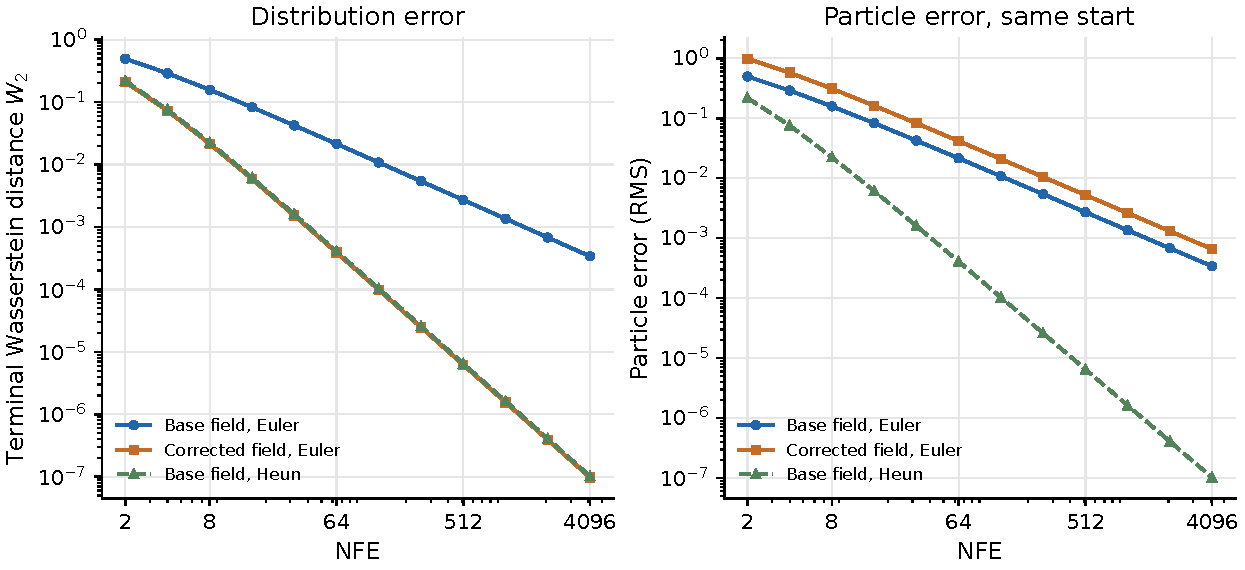
\includegraphics[width=\linewidth]{../results/figures/equal_evaluation.pdf}
\caption{Corrected Euler closely matches base-field Heun in nonlinear distribution error at equal NFE, although it has larger particle error. The source and parameters are those of Figure~\ref{fig:nonlinear}, and each even $N$ gives $N$ uniform Euler steps or $N/2$ Heun steps of twice the length. The left and right panels compare distribution and particle errors, respectively. Base-field Heun has particle error equal to $W_2$.}
\label{fig:equal-evaluation}
\end{figure}

\begin{table}[t]
\centering
\caption{At these low NFE values, corrected Euler has slightly smaller distribution error and larger particle error than base-field Heun. The setup is that of Figure~\ref{fig:nonlinear}, and the displayed $W_2$ equals particle error for both base-field methods. The final column gives the ratio of corrected Euler to base-field Heun distribution error, calculated from unrounded values.}
\label{tab:few-evaluations}
\par\smallskip
\begin{tabular}{rccccc}
\toprule
NFE & \shortstack{Base field\\Euler $W_2$} & \shortstack{Corrected field\\Euler $W_2$} & \shortstack{Base field\\Heun $W_2$} & \shortstack{Corrected field\\Euler particle error} & \shortstack{Corrected Euler /\\base-field Heun $W_2$} \\
\midrule
2 & $4.96\times10^{-1}$ & $2.11\times10^{-1}$ & $2.18\times10^{-1}$ & $9.82\times10^{-1}$ & 0.9671 \\
4 & $2.89\times10^{-1}$ & $7.25\times10^{-2}$ & $7.54\times10^{-2}$ & $5.74\times10^{-1}$ & 0.9609 \\
8 & $1.58\times10^{-1}$ & $2.14\times10^{-2}$ & $2.24\times10^{-2}$ & $3.11\times10^{-1}$ & 0.9570 \\
16 & $8.26\times10^{-2}$ & $5.84\times10^{-3}$ & $6.11\times10^{-3}$ & $1.62\times10^{-1}$ & 0.9548 \\
\bottomrule
\end{tabular}

\end{table}

With the rotation $b=a/\sqrt3$, Heun has third-order distribution error while particle error remains second order. We compare this corrected Heun method with Kutta's third-order Runge--Kutta method, denoted RK3, on the base field at equal NFE. Corrected Heun has 18.0--20.9\% smaller distribution error at 12, 48, 192, and 384 NFE, although its particle error is larger. Appendix Table~\ref{tab:gaussian-higher-order} gives the values. Appendix~\ref{app:heun-rk3} derives the coefficients, and Appendix Figure~\ref{fig:solver} shows convergence.

\subsection{A residual acceleration adds a first-order term to the bound}

An imperfect correction can keep the probability path unchanged without fully satisfying the acceleration condition. Write $\acc_t=w_t+g_t$, where $w_t$ satisfies Eq.~\eqref{eq:flux-null} under $p_t$ and $g_t$ is the residual. Shifting the starting points along $w_t$ supplies the part of Euler's missing displacement that preserves the distribution. The contribution from $g_t$ remains.
\begin{proposition}[Residual acceleration]
\label{prop:robustness}
Keep the assumptions on $u$ and $C_j$ from Theorem~\ref{thm:distribution_order}. Assume that $w_t$ is $C^1$, globally Lipschitz with common constant $L_w$, and satisfies Eq.~\eqref{eq:flux-null} under $p_t$. If
$C_{w,2}=\sup_t\|w_t\|_{L^2(p_t)}<\infty$ and
$\sup_t\|g_t\|_{L^2(p_t)}\le\varepsilon$, then
\begin{equation}
 \max_kW_2(\widehat p_k,p_{t_k})
 \le e^{LT}T\left(C_wH^2+\tfrac12\varepsilon H\right),
 \qquad C_w=\frac{C_j}{6}+\frac{LC_{w,2}}{2}+\frac{TL_wC_{w,2}}{8}.
 \label{eq:robustness}
\end{equation}
\end{proposition}

In each step, the residual adds at most $\varepsilon h^2/2$ to the root mean squared distance between the paired points. Adding these contributions over the steps gives the $\varepsilon H$ term. If the other constants stay bounded, $\varepsilon=O(H)$ is enough for second-order accuracy. For example, halving both $H$ and $\varepsilon$ divides both terms in $H^2+\varepsilon H$ by four. Halving only $H$ divides the residual term by two. A fixed residual leaves a first-order term in the bound, but this does not mean that the actual error is always first order. Appendix~\ref{app:robustness} proves the bound and gives the sum over individual steps.

In the nonlinear example, a fixed mismatch in rotation gives first-order error. Replacing $\beta$ by $\lambda\beta$, with $\lambda\ge0$ fixed as the grid is refined, keeps the probability path unchanged but gives acceleration
\[
 \acc_{u_\lambda}(x)=(1-\lambda^2)P(r)x+\lambda\beta_a(r)Jx.
\]
For $\lambda\ne1$, the remaining radial acceleration leads to
$W_2(\widehat p_N^\lambda,p_T)/h\to|1-\lambda^2|\kappa_0>0$,
as proved in Appendix~\ref{app:nonlinear-sensitivity}. Even a small fixed mismatch therefore gives first-order convergence. It can still reduce error compared with the base field over a finite range of step sizes.

We can estimate where the mismatch starts to matter by equating its leading contribution $|1-\lambda^2|\kappa_0h$ with the exact correction's contribution $\kappa_1h^2$. This gives
\[
 h_*\approx |1-\lambda^2|\frac{\kappa_0}{\kappa_1}.
\]
For the Gaussian path, the corresponding coefficients are $c_0^{\rm G}=C_\Sigma a^2T/2$ and $c_1^{\rm G}=2C_\Sigma a^3T/3$, where $C_\Sigma=e^{aT}\sqrt{\tr\Sigma_0}$. They give $h_*^{\rm G}\approx |1-\lambda^2|c_0^{\rm G}/c_1^{\rm G}=3|1-\lambda^2|/(4a)$. At $a=0.6$ on $[0,1]$, the 2\% mismatches $\lambda=0.98$ and $1.02$ give about $20$ steps, as shown in Appendix Figure~\ref{fig:sensitivity}. The first-order error dominates at sufficiently smaller step sizes. When $\lambda>1$, the two contributions can have opposite signs and cancel near this estimate. Thus the estimate gives a range where both terms matter, rather than an exact threshold between orders.

\FloatBarrier

The appendices give the proofs and numerical details for the paper. In the Gaussian example, distribution error depends on scale, while particle error also depends on angle. The nonlinear example shows the same difference when the distribution changes shape. The general proof shows how the acceleration condition improves distribution accuracy in both examples. The table below gives the location of each result.

\begin{center}
\begin{tabular}{p{0.70\linewidth}l}
\toprule
Main claim or comparison & Support\\
\midrule
Finite-time $W_2$ bound and its coupling & Appendix~\ref{app:general}\\
Minimum action and the gradient-field consequence & Appendix~\ref{app:projection}\\
Gaussian distribution and particle errors & Appendix~\ref{app:fixed-gaussian}\\
Nonlinear rates, coefficient error, and extensions & Appendix~\ref{app:nonlinear}\\
Residual acceleration bound & Appendix~\ref{app:robustness}\\
Local converse and terminal cancellation & Appendix~\ref{app:local}\\
Solver dependence and equal NFE & Appendix~\ref{app:solver}\\
Mean, second-moment, and action restrictions & Appendix~\ref{app:obstruction}\\
Scaled rotated Gaussian coupling & Appendix~\ref{app:fm}\\
Weak expansion and regular displacement interpolation & Appendices~\ref{app:weak}, \ref{app:displacement}\\
Arbitrarily small action cost on one grid & Appendix~\ref{app:schedules}\\
Population calculations and refinement results & Appendix~\ref{app:numerics}\\
\bottomrule
\end{tabular}
\end{center}

For a map $F$, the pushforward $F_\#\mu$ is the distribution of $F(X)$ when $X\sim\mu$. We write $\mathcal P_2(\R^d)$ for probability measures with finite second moment, and define the root mean squared size of a vector field $w$ by
\[
 \|w\|_{L^2(p)}=\left(\int \|w(x)\|^2p(\dd x)\right)^{1/2}.
\]
For a random vector $Z$, $\|Z\|_{L^2}$ is its root mean squared norm. Table~\ref{tab:notation} lists the main symbols.

\begin{table}[ht]
\centering
\caption{Notation used in the proofs. Matrices and coefficients specific to an example are defined with that example.}
\label{tab:notation}
\begin{tabular}{lp{0.73\linewidth}}
\toprule
Symbol & Meaning\\
\midrule
$p_t$, $\widehat p_k$ & Exact distribution at time $t$ and Euler distribution at node $k$\\
$u_t$, $r_t$ & Velocity field and a correction added to that field\\
$\acc_t$, $\jerk_t$ & Second and third time derivatives along an exact particle\\
$T$, $h_k$, $H$ & Final time, step length, and largest step length\\
$W_2$ & Distribution distance from the best root mean squared pairing\\
$\cA_T$ & Kinetic action over the time interval $[0,T]$\\
$F_{s,t}$ & Exact particle flow from time $s$ to time $t$\\
$\Psi_t^\tau$ & Auxiliary acceleration flow with physical time $t$ held fixed\\
$L$, $L_a$ & Common spatial Lipschitz bounds for velocity and acceleration\\
$C_a$, $C_j$ & Uniform $L^2(p_t)$ bounds for acceleration and its material derivative\\
$\Sigma_0$, $\Omega$ & Initial Gaussian covariance and its weighted rotation matrix\\
$C_0$, $K_t$ & Gaussian covariance root and skew matrix in the rotation representation\\
$C_{w,2}$, $C_w$ & $L^2$ bound for $w_t$ and constant in the residual bound\\
$\alpha$, $\beta$, $\beta_a$ & Nonlinear radial rate, rotation rate, and tangential acceleration coefficient\\
$\mathcal C_i$, $\Theta_1$ & Leading radius-error and angle-error coefficient functions\\
$\mathcal T$, $G$, $d_{\rm aff}$ & Affine map, its matrix, and its shift\\
$R(t,r)$, $R_{i,k}(r)$ & Exact and numerical radii from starting radius $r$\\
\bottomrule
\end{tabular}
\end{table}
\FloatBarrier

\section{Fixed Gaussian correction and recursive errors}
\label{app:fixed-gaussian}

The Gaussian result also holds when the mean moves at constant velocity and the covariance is any positive definite matrix in even dimension. Assume $T,a>0$ and $\Sigma_0=C_0C_0^\top$, with $J^\top=-J$, $J^\top J=I$, and $\Omega=C_0JC_0^{-1}$. For $m_t=m_0+t\xi$, the fields $v_0(t,x)=\xi+a(x-m_t)$ and $v_1(t,x)=\xi+a(I+\Omega)(x-m_t)$ both generate $p_t=\mathcal N(m_t,e^{2at}\Sigma_0)$. These parameters stay fixed as the grid changes. The base field $v_0$ minimizes action among finite-action fields satisfying the same weak continuity equation. The correction increases action by
\[
 \cA_T(v_1)-\cA_T(v_0)=a^2\tr(\Sigma_0)\frac{e^{2aT}-1}{2a}>0.
\]
Euler reproduces $m_t$ exactly and has covariance $q_{i,k}\Sigma_0$, where
\[
 q_{0,k}=\prod_{j<k}(1+ah_j)^2,\qquad
 q_{1,k}=\prod_{j<k}(1+2ah_j+2a^2h_j^2).
\]
Euler's distribution error is $\sqrt{\tr(\Sigma_0)}[e^{at_k}-\sqrt{q_{i,k}}]$. The corrected error is positive and strictly smaller for every $k\ge1$. Equations~\eqref{eq:base-order}--\eqref{eq:particle-order} hold with $C_\Sigma=\sqrt{\tr(\Sigma_0)}e^{aT}$. Setting $m_0=\xi=0$ and $\Sigma_0=I_2$ gives Theorem~\ref{thm:fixed-gaussian}.

Write
\[
 I_a(T)=\int_0^T e^{2at}\dd t=\frac{e^{2aT}-1}{2a}.
\]
Subtracting the mean and applying the inverse covariance factor gives a Gaussian source with identity covariance. These coordinates are called whitened coordinates. Each corrected Euler step changes scale and angle, but rotation leaves the Gaussian distribution unchanged. Distribution error therefore depends only on scale. Particles from the same starting point also have an angle error. The scale error has a positive second-order coefficient, while the angle error has a positive first-order coefficient.

The correction belongs to the Gaussian family of \citet[Proposition~5.5]{lim2025hidden}. For a single Gaussian with $\Sigma_t=e^{2at}C_0C_0^\top$, the skew matrix $K_t=b e^{-2at}C_0^{-\top}JC_0^{-1}$ gives $\Sigma_tK_t(x-m_t)=b\Omega(x-m_t)$. This form lets us calculate kinetic action and Euler error over the full time interval.

\begin{proof}[Proof of Theorem~\ref{thm:fixed-gaussian} and its Gaussian extension]
\label{proof:fixed-gaussian}
\textbf{Common path and action.}\quad
The assumptions on $J$ imply $J^2=-I$. Direct matrix multiplication verifies
\[
 \Omega\Sigma_t+\Sigma_t\Omega^\top=0,\qquad
 \Omega\Sigma_t\Omega^\top=\Sigma_t,\qquad \Sigma_t=e^{2at}\Sigma_0.
\]
The centered flows $e^{at}I$ and $e^{at}C_0e^{atJ}C_0^{-1}$ both give covariance $\Sigma_t$ and mean $m_t$. Both flows are global and affine, so the distributions remain Gaussian. Equal means and covariances therefore give the same distribution at every intermediate time.

For $Y\sim\mathcal N(0,\Sigma_t)$, we have $\mathbb E\|\Omega Y\|^2=\operatorname{tr}(\Sigma_t)$ and $\mathbb E[Y^\top \Omega Y]=\operatorname{tr}(\Omega\Sigma_t)=0$, since $\Omega\Sigma_t$ is skew. The cross terms with $\xi$ also have zero expectation because $Y$ is centered. Expanding the squared speed and integrating over time therefore gives the action identities.

The base field is the gradient of $\xi^\top x+(a/2)\|x-m_t\|^2$. This potential has quadratic growth, so the projection argument in Appendix~\ref{app:projection} applies. The base field uniquely minimizes action up to almost-everywhere equality. For the continuous fields in the class $\cV(p)$ defined there, positive Gaussian density gives equality at every time and position. In particular,
\[
 \cA_T(v_0)=T\|\xi\|^2+a^2\tr(\Sigma_0)I_a(T).
\]

\textbf{Recursive covariance and strict improvement.}\quad
Let $r_{i,k}=\sqrt{q_{i,k}}$ and $\widehat p_k^i=\widehat p_k^{v_i}$ for $i=0,1$. Euler reproduces the affine mean exactly, while its centered whitened matrices are $(1+ah_j)I$ and $(1+ah_j)I+ah_jJ$. The second matrix multiplied by its transpose is $(1+2ah_j+2a^2h_j^2)I$, so repeated covariance updates give the product formulas. For equal-mean Gaussians with covariances $r^2\Sigma_0$ and $s^2\Sigma_0$, $W_2$ equals $|r-s|\sqrt{\operatorname{tr}(\Sigma_0)}$.

For $z>0$,
\[
 (1+z)^2<1+2z+2z^2<e^{2z}.
\]
The first difference is $z^2$, while the second inequality follows from the positive remaining terms in the exponential series. Taking square roots and multiplying over the steps gives $r_{0,k}<r_{1,k}<e^{at_k}$ for every $k\ge1$. Both numerical distributions have too small a scale, but the corrected scale is closer to the exact value. The corrected error is strictly smaller at every grid point, so its maximum and sum are also smaller.

\textbf{Accumulated error and convergence rates.}\quad
To find the convergence orders, we calculate the scale error over all steps. Taking logarithms changes the product of step factors into a sum. The positive error terms for each step are
\[
 f_0(z)=z-\log(1+z),\qquad
 f_1(z)=z-\tfrac12\log(1+2z+2z^2).
\]
Their derivatives are
\[
 f_0'(z)=\frac{z}{1+z},\qquad
 f_1'(z)=\frac{2z^2}{1+2z+2z^2}.
\]
Integrate from zero to obtain
$0<f_0(z)\le z^2/2$ and $0<f_1(z)\le2z^3/3$.
Put $\Delta^{\mathrm{log}}_{i,k}=\sum_{j<k}f_i(ah_j)$.
Then $r_{i,k}=e^{at_k}e^{-\Delta^{\mathrm{log}}_{i,k}}$ and
\[
 W_2(\widehat p^i_k,p_{t_k})
 =\sqrt{\operatorname{tr}(\Sigma_0)}e^{at_k}(1-e^{-\Delta^{\mathrm{log}}_{i,k}}).
\]
Use $1-e^{-\Delta^{\mathrm{log}}}\le \Delta^{\mathrm{log}}$, $\sum_{j<k}h_j^2\le t_kH$, and
$\sum_{j<k}h_j^3\le t_kH^2$ to obtain the explicit unequal-step bounds
\[
 \max_kW_2(\widehat p_k^0,p_{t_k})
 \le\sqrt{\tr\Sigma_0}e^{aT}\frac{a^2T}{2}H,
 \qquad
 \max_kW_2(\widehat p_k^1,p_{t_k})
 \le\sqrt{\tr\Sigma_0}e^{aT}\frac{2a^3T}{3}H^2.
\]

Near zero,
\[
 f_0(z)=\tfrac12z^2-\tfrac13z^3+O(z^4),\qquad
 f_1(z)=\tfrac23z^3-z^4+O(z^5).
\]
On the uniform grid,
\[
 \Delta^{\mathrm{log}}_{0,N}=\frac{a^2T}{2}h+O(h^2),\qquad
 \Delta^{\mathrm{log}}_{1,N}=\frac{2a^3T}{3}h^2+O(h^3).
\]
Substitute these expansions into $1-e^{-\Delta^{\mathrm{log}}}=\Delta^{\mathrm{log}}+O((\Delta^{\mathrm{log}})^2)$ to obtain the terminal expansions.
\end{proof}

\begin{proposition}[Particle error for the fixed correction]
\label{prop:gaussian-particle-error}
Pair the exact and numerical particles for $v_1$ through the same
$X_0\sim p_0$. On a uniform grid, set
\[
 r_N=(1+2ah+2a^2h^2)^{N/2},\qquad
 \theta_N=N\arctan\frac{ah}{1+ah}.
\]
Their terminal mean squared difference is
\[
 \mathbb E\|\widehat X_N-X_T\|^2
 =\operatorname{tr}(\Sigma_0)
 \left[(r_N-e^{aT})^2
       +4r_Ne^{aT}\sin^2\frac{\theta_N-aT}{2}\right].
\]
Consequently, their root mean squared difference satisfies
\[
 \left(\mathbb E\|\widehat X_N-X_T\|^2\right)^{1/2}
 =\sqrt{\operatorname{tr}(\Sigma_0)}e^{aT}a^2T\,h+O(h^2).
\]
\end{proposition}

\begin{proof}
Particle error compares the exact and numerical maps from the same starting vector, so it includes their angle difference. In whitened coordinates these maps are $e^{aT}e^{aTJ}$ and $r_Ne^{\theta_NJ}$. The difference multiplied by its transpose is a scalar matrix with factor $r_N^2+e^{2aT}-2r_Ne^{aT}\cos(\theta_N-aT)$. Multiplication by $C_0$ and $C_0^\top$ makes its trace equal to this factor times the initial covariance trace, proving the formula. The numerical mean is exact.

Expanding the numerical angle shows that
\[
 \theta_N-aT=-a^2T h+O(h^2).
\]
The radial scale difference is $O(h^2)$ by the theorem. The angle difference is first order and gives the leading particle error through the sine term. An optimal distribution pairing matches angles, so the angle difference does not contribute to $W_2$.
\end{proof}


\section{A distribution bound over a fixed time interval}
\label{app:general}

We bound distribution error by moving Euler's starting point along the acceleration field while holding physical time fixed. If this motion preserves the starting distribution, Euler gives the same output distribution. Its output can then be paired more closely with exact motion from the original starting point. Zero weighted divergence ensures that the starting distribution stays exactly the same. A suitable shift supplies the leading displacement that Euler omits. Preserving selected averages, or preserving the distribution only to first order, would not be enough for this coupling.

Let $F_{s,t}$ be the exact flow of $u$, and let $p_t=(F_{0,t})_\#p_0$. Define
\[
 \acc_t=\partial_tu_t+(D_xu_t)u_t,
 \qquad \jerk_t=\partial_t\acc_t+(D_x\acc_t)u_t.
\]
These fields are the second and third time derivatives along an exact particle. A field $w$ has \emph{zero weighted divergence under} a measure $p$ if
\begin{equation}
 \int w\cdot\nabla\phi\,\dd p=0
 \quad\text{for every }\phi\in C_c^\infty(\R^d).
 \label{eq:appendix-flux-null}
\end{equation}
The tests in $C_c^\infty$ are smooth and vanish outside a bounded set. The definition therefore applies even when the measure has no density. If a density exists, the condition is the weak form of $\nabla\!\cdot(pw)=0$. The auxiliary flow is autonomous, which means that its field stays fixed as auxiliary time changes.

\begin{proposition}[Preservation with physical time fixed]
\label{prop:frozen-preservation}
Let $p$ be a probability measure and let $w\in C^1(\R^d;\R^d)$ be globally Lipschitz. If $w$ has zero weighted divergence under $p$, its autonomous flow $\Psi^\tau$ satisfies $(\Psi^\tau)_\#p=p$ for every $\tau\in\R$.
\end{proposition}
\begin{proof}
Global Lipschitz continuity gives a flow at all positive and negative times, with $\Psi^\tau$ a $C^1$ diffeomorphism and inverse $\Psi^{-\tau}$. For a smooth compactly supported test $\phi$, the support of $\phi\circ\Psi^\tau$ lies in the image of the support of $\phi$ under this continuous inverse. The composition therefore has compact support and is $C^1$, although it need not be infinitely differentiable. Convolution extends Eq.~\eqref{eq:appendix-flux-null} to $C_c^1$ tests, so it applies to the composition.

The autonomous flow satisfies $D\Psi^\tau(x)w(x)=w(\Psi^\tau(x))$. For $\phi\in C_c^\infty$,
\[
 \frac{\dd}{\dd\tau}\int\phi(\Psi^\tau(x))p(\dd x)
 =\int w(x)\cdot\nabla(\phi\circ \Psi^\tau)(x)p(\dd x)=0.
\]
On each bounded time interval, one compact set contains the supports of these integrands, where both the integrands and their derivatives are bounded. Differentiation under the integral is therefore valid. The derivative is zero, so every test expectation stays constant and the measures are equal.
\end{proof}

Because the auxiliary flow preserves the distribution exactly, we can form a coupling with local error bounded by a constant times $h^3$. Euler's Lipschitz bound then controls how much later steps increase this error. We restate Theorem~\ref{thm:distribution_order} with the assumptions needed for these two estimates.

\begin{quote}
\textbf{Theorem~\ref{thm:distribution_order}, restated.}
Let $T>0$ and $p_0\in\mathcal P_2(\R^d)$. Suppose $u$ is $C^2$ on a neighborhood of $[0,T]\times\R^d$, globally Lipschitz in space with a common constant $L$, and $\sup_{t\in[0,T]}\|u(t,0)\|<\infty$. Suppose each $\acc_t$ is globally Lipschitz with a common constant $L_a$ and has zero weighted divergence under $p_t$. Assume
\[
 C_a=\sup_{0\le t\le T}\|\acc_t\|_{L^2(p_t)}<\infty,
 \qquad C_j=\sup_{0\le t\le T}\|\jerk_t\|_{L^2(p_t)}<\infty.
\]
For every finite increasing grid $0=t_0<\cdots<t_N=T$, put $h_k=t_{k+1}-t_k$, $H=\max_kh_k$, and $E_{t,h}(x)=x+hu(t,x)$. Euler's method means
\[
 \widehat p_0=p_0,\qquad
 \widehat p_{k+1}=(E_{t_k,h_k})_\#\widehat p_k.
\]
Then
\begin{equation}
 \begin{aligned}
 \max_{0\le k\le N}W_2(\widehat p_k,p_{t_k})
 &\le e^{LT}\left(\frac{C_j}{6}+\frac{LC_a}{2}+\frac{TL_aC_a}{8}\right)
       \sum_{j=0}^{N-1}h_j^3\\
 &\le e^{LT}\left(\frac{C_j}{6}+\frac{LC_a}{2}+\frac{TL_aC_a}{8}\right)TH^2.
 \end{aligned}
 \label{eq:general-bound-full}
\end{equation}
\end{quote}

\begin{proof}[Proof of Theorem~\ref{thm:distribution_order}]
\label{proof:distribution-order}
The growth and Lipschitz assumptions give an exact flow on the full interval with finite second moments. For $X\sim p_t$, Taylor's formula shows the displacement that Euler omits:
\[
 F_{t,t+h}(X)=X+hu_t(X)+\frac{h^2}{2}\acc_t(X)+\rho_{t,h}.
\]
The remainder integrates the third trajectory derivative, which has the stated $L^2$ bound because the intermediate distribution is $p_{t+s}$. Minkowski's inequality gives
\begin{equation}
 \|\rho_{t,h}\|_{L^2}
 \le\frac12\int_0^h(h-s)^2
       \|\jerk_{t+s}(X_{t+s})\|_{L^2}\dd s
 \le\frac{C_j}{6}h^3.
 \label{eq:flow-remainder-l2}
\end{equation}
Let $\Psi_t^\tau$ be the flow of $\acc_t$ with physical time $t$ fixed. By Proposition~\ref{prop:frozen-preservation}, $\Psi_t^\tau X\sim p_t$ for every auxiliary time $\tau$, so the bound $C_a$ applies throughout the motion. Integrating acceleration bounds the displacement, while integrating its change from the initial value bounds the remainder. For $\tau\ge0$,
\[
 \|\Psi_t^\tau X-X\|_{L^2}\le C_a\tau,
 \qquad
 \|\Psi_t^\tau X-X-\tau\acc_t(X)\|_{L^2}
 \le\int_0^\tau L_aC_av\dd v=\frac{L_aC_a}{2}\tau^2.
\]
Choose $\tau=h^2/2$. Euler's output from the shifted start still has distribution $(E_{t,h})_\#p_t$. Pairing this output with $F_{t,t+h}(X)$ gives the Wasserstein bound
\begin{align}
 \Psi_t^{h^2/2}X&=X+\tfrac12h^2\acc_t(X)+O_{L^2}(h^4),\nonumber\\
 W_2((E_{t,h})_\#p_t,p_{t+h})
 &\le\|E_{t,h}(\Psi_t^{h^2/2}X)-F_{t,t+h}(X)\|_{L^2}\nonumber\\
 &\le\frac{L_aC_a}{8}h^4+\frac{LC_a}{2}h^3+\frac{C_j}{6}h^3.
 \label{eq:coupling-bound}
\end{align}
The shift supplies $\tau\acc_t(X)$, which is the second-order displacement in the exact expansion. It also changes the point at which Euler evaluates velocity, producing the difference $h[u_t(\Psi_t^\tau X)-u_t(X)]$. Since the shift is $O(h^2)$ in root mean square, the spatial Lipschitz bound makes this additional displacement $O(h^3)$.

This local estimate starts from the exact distribution. In a sequence of Euler steps, we must also bound error from earlier steps. For a Lipschitz map $E$ and measures $\mu,\nu\in\mathcal P_2$, apply $E$ to both members of a coupling and take the infimum over couplings. This gives $W_2(E_\#\mu,E_\#\nu)\le\operatorname{Lip}(E)W_2(\mu,\nu)$. For Euler, $\operatorname{Lip}(E_{t,h})\le1+Lh$. With $e_k=W_2(\widehat p_k,p_{t_k})$ and $C_*=C_j/6+LC_a/2+TL_aC_a/8$, the triangle inequality separates the earlier error from the new local error. Since $h_k\le T$,
\begin{align*}
 e_{k+1}&\le W_2((E_{t_k,h_k})_\#\widehat p_k,(E_{t_k,h_k})_\#p_{t_k})\\
 &\quad+W_2((E_{t_k,h_k})_\#p_{t_k},p_{t_{k+1}})\\
 &\le(1+Lh_k)e_k+C_*h_k^3.
\end{align*}
Starting from $e_0=0$, we apply this inequality at each step. Later steps increase each local error by at most $\prod_j(1+Lh_j)\le e^{LT}$. The sum satisfies $\sum_jh_j^3\le H^2\sum_jh_j=TH^2$, which gives the claimed order.
\end{proof}

If the initial numerical distribution differs from $p_0$, the same proof adds
$e^{LT}W_2(\widehat p_0,p_0)$ to the right side. 

\paragraph{The modified equation.}
The modified equation produces the same cancellation by changing the velocity field. For a fixed step parameter $h$, let $Y_s$ solve $\dot Y_s=u(t+s,Y_s)-(h/2)\acc(t+s,Y_s)$ from $Y_0=x$ over $0\le s\le h$. Physical time evolves while $h$ remains fixed. On compact sets, $u\in C^2$ and $\acc\in C^1$ give $Y_s=x+s u(t,x)+O(hs+s^2)$, and substitution yields
\[
 u(t+s,Y_s)=u(t,x)+s\acc(t,x)+O(hs+s^2),\qquad
 \acc(t+s,Y_s)=\acc(t,x)+O(s).
\]
After integration, the terms $h^2\acc(t,x)/2$ cancel, giving $Y_h=x+hu(t,x)+O(h^3)$. For sufficiently small $h$, the remainders are uniform on compact sets. This is the first field correction in backward error analysis~\citep[Chapter~IX]{hairer2006geometric}. Under the theorem's global assumptions, $u-(h/2)\acc$ has a unique global flow. The acceleration condition leaves the weak continuity equation unchanged, so uniqueness gives the same distribution as $u$ at every time. The expansion on compact sets alone does not bound mean squared error for an unbounded source. The coupling proof gives the integrable estimates needed for the finite-time bound.

\section{A necessary local condition and terminal cancellation}
\label{app:local}

If one Euler step from the exact distribution has error $o(h^2)$, the field must satisfy the acceleration condition at that time. Terminal accuracy on a family of grids does not imply this local condition, because errors from different times can cancel. We prove the local result and then give an example of terminal cancellation.

\begin{quote}
\textbf{Proposition~\ref{prop:local-converse}, restated.}
Let $u$ and $p_t$ satisfy the smoothness, growth, Lipschitz, and moment assumptions of Theorem~\ref{thm:distribution_order}, without requiring zero weighted divergence of acceleration under the current distribution. At a fixed $t<T$, suppose
\[
 W_2((E_{t,h})_\#p_t,p_{t+h})=o(h^2)
 \quad\text{as }h\downarrow0.
\]
Then $\acc_t$ has zero weighted divergence under $p_t$.
\end{quote}
\begin{proof}[Proof of Proposition~\ref{prop:local-converse}]
\label{proof:local-converse}
For $X\sim p_t$, compare one Euler step $Y=E_{t,h}X$ with exact motion $Y+\Delta X$, where $\Delta X=F_{t,t+h}X-Y=h^2\acc_t(X)/2+\rho_{t,h}$. Equation~\eqref{eq:flow-remainder-l2} gives $\|\rho_{t,h}\|_{L^2}=O(h^3)$ and $\|\Delta X\|_{L^2}=O(h^2)$. Since a smooth compactly supported test $\phi$ has bounded first and second derivatives, Taylor expansion gives
\[
 \E[\phi(Y)-\phi(Y+\Delta X)]
 =-\E[\nabla\phi(Y)\cdot \Delta X]+O(\E\|\Delta X\|^2).
\]
Replacing $\Delta X$ by $h^2\acc_t(X)/2$ changes the expectation by $O(h^3)$. Replacing $\nabla\phi(Y)$ by $\nabla\phi(X)$ changes it by at most
$Ch^3\|u_t\|_{L^2(p_t)}\|\acc_t\|_{L^2(p_t)}$. Hence
\begin{equation}
 \E\phi(E_{t,h}X)-\E\phi(F_{t,t+h}X)
 =-\frac{h^2}{2}\int\nabla\phi\cdot\acc_t\dd p_t+o(h^2).
 \label{eq:local-second-moment-expansion}
\end{equation}
The expectation difference has absolute value at most $\operatorname{Lip}(\phi)W_2((E_{t,h})_\#p_t,p_{t+h})$, which tends to zero after division by $h^2$. The acceleration integral is therefore zero for every smooth compactly supported test, which proves zero weighted divergence. The moment requirements are the finite second moment and the stated $L^2$ bounds on acceleration and jerk, with $C_j$ controlling the trajectory remainder through Eq.~\eqref{eq:flow-remainder-l2}.
\end{proof}

Conversely, under all assumptions and common bounds in Appendix~\ref{app:general}, zero weighted divergence of acceleration gives local $O(h^3)$ error. Both directions concern one step started from the exact distribution.

For a terminal counterexample, let $T=1$, $p_0=\mathcal N(0,I_d)$, and
\[
 u(t,x)=\sin(2\pi t)e_1.
\]
Here $e_1$ is the first coordinate vector. The particles translate in this direction during the first half of the interval and return during the second half, giving zero exact terminal displacement. Euler also gives zero displacement on every uniform grid with $N\ge1$ steps, since
\[
 \frac1N\sum_{k=0}^{N-1}\sin(2\pi k/N)e_1=0.
\]
For $N>1$, summing the $N$th roots of unity and taking imaginary parts gives this identity, while $N=1$ follows directly. However, $\acc_t=2\pi\cos(2\pi t)e_1$ has nonzero weighted divergence whenever it is nonzero. The current distribution is a translated Gaussian, whose density has a nonzero derivative along any nonzero constant direction. Thus terminal exactness does not imply the local condition.

\subsection{Weak expansion with an explicit remainder}
\label{app:weak}

Weak error compares expectations of test functions. We calculate its leading term and give an explicit cubic remainder for $C_b^3$ tests. These tests have continuous bounded values and derivatives through order three. This larger test class requires a stronger moment assumption than the local converse. The expansion alone does not bound $W_2$. The coupling in Appendix~\ref{app:general} gives that bound under the assumptions stated there.

\begin{proposition}[Local weak error of Euler]
\label{prop:weak-euler}
Fix $t$ and $h_0>0$. Suppose $u$ is $C^2$ on a neighborhood of $[t,t+h_0]\times\R^d$, and one constant $C$ satisfies
\begin{align*}
 \|u(s,x)\|+\|\partial_su(s,x)\|+\|\partial_s^2u(s,x)\|&\le C(1+\|x\|),\\
 \|D_xu(s,x)\|_{\rm op}+\|D_x\partial_su(s,x)\|_{\rm op}+\|D_x^2u(s,x)\|_{\rm op}&\le C.
\end{align*}
Let $X\sim p_t$ have finite third moment, let $p_{t+h}$ be its exact evolved law, and let $\phi\in C_b^3(\R^d)$. Then
\[
 \E\phi(X+hu_t(X))-\E_{p_{t+h}}\phi
 =-\frac{h^2}{2}\E_{p_t}[\nabla\phi\cdot\acc_t]+R_h,
 \qquad |R_h|\le C_{\rm weak}h^3\E(1+\|X\|^3).
\]
The constant $C_{\rm weak}$ depends on $C$, $h_0$, and the supremum norms of $\nabla\phi$, $D^2\phi$, and $D^3\phi$, but not on $h$.
\end{proposition}
\begin{proof}
The numerical and exact test expansions agree at first order. Gronwall's inequality bounds the exact position by a constant times one plus the source radius, while acceleration has at most linear growth. Its derivative along the exact flow is
\[
 \jerk=\partial_t^2u+2(D_x\partial_tu)u+D_x^2u[u,u]
 +(D_xu)\partial_tu+(D_xu)^2u.
\]
This derivative has at most quadratic growth. Taylor's formula along the straight Euler step is
\[
 \phi(x+hu_t(x))=\phi(x)+h\nabla\phi\cdot u_t
 +\frac{h^2}{2}D^2\phi[u_t,u_t]+O(h^3(1+\|x\|^3)).
\]
Along the exact flow the second derivative of the test is
$D^2\phi[u,u]+\nabla\phi\cdot\acc$, and its third derivative is
$D^3\phi[u,u,u]+3D^2\phi[u,\acc]+\nabla\phi\cdot\jerk$.
The derivative and flow bounds make this third derivative at most $C_{\rm weak}(1+\|x\|^3)$ in absolute value. Subtracting the expansions cancels the terms that depend only on velocity and leaves the stated acceleration term. The finite third moment makes the remainder integrable.
\end{proof}

For smooth tests with compact support, integration by parts expresses the leading difference between the two distributions as
\[
 (\mathrm{Id}+hu_t)_\#p_t-p_{t+h}
 =\frac{h^2}{2}\nabla\!\cdot(p_t\acc_t)+O_{\mathrm{weak}}(h^3).
\]
The equality holds after integration against smooth compactly supported tests, up to the stated weak remainder. Integration by parts changes the sign of the acceleration integral and gives the positive divergence coefficient. When acceleration has zero weighted divergence, cutoff approximation extends this cancellation to the bounded tests in the proposition because acceleration is integrable.

For quadratic tests, the Euler expansion stops at order two, while the third derivative along the exact flow grows at most cubically. The third-moment assumption therefore makes the same formula valid. For affine fields $u(s,x)=B(s)x+d_{\rm aff}(s)$ with bounded coefficient derivatives through order two, this growth is only quadratic, so a finite second moment suffices for quadratic tests, including mean and covariance entries.

For the fixed Gaussian correction, write $y=x-m_t$ and $B=a(I+\Omega)$. The time derivative $-B\xi$ cancels the constant part $B\xi$ in $(D_xu)u$. Thus
\[
 \acc_{v_1}=B^2y=2a^2\Omega y.
\]
The matrix identities imply $\tr \Omega=0$ and skew-symmetry of $\Sigma_t^{-1}\Omega$. Hence the Gaussian density satisfies
\[
 \nabla\!\cdot(p_t\Omega y)
 =p_t[\tr \Omega-y^\top\Sigma_t^{-1}\Omega y]=0.
\]
Acceleration is nonzero away from the mean, but its weighted divergence is zero. The leading weak error therefore cancels. The Gaussian covariance recursion gives the convergence rate directly, while the coupling theorem bounds distribution error for more general distributions. Proposition~\ref{prop:local-converse} shows that the local condition is necessary under the stated second-moment, acceleration, and jerk bounds.

\section{A nonlinear radial path and its exact error coefficients}
\label{app:nonlinear}

For a nonlinear radial path, covariance is not enough to determine the distribution. We therefore calculate distribution error from the full distribution of radii. Radial symmetry gives an optimal coupling that matches angles and pairs radii in increasing order. We show that the numerical radius maps keep this order and calculate their error over all steps. Bounds valid at every source radius then let us take expectations of the error limits. To calculate particle error, we also include the angle difference between particles from the same starting point.

For Theorem~\ref{thm:nonlinear}, assume $a,\eta,T>0$. Let $p_0$ be rotationally invariant on $\R^2$, with $m_{2,0}=\int \|x\|^2p_0(\dd x)\in(0,\infty)$. A density is not required. Define
\begin{align*}
 J&=\begin{pmatrix}0&-1\\1&0\end{pmatrix},&
 \alpha(r)&=a+\eta\frac{r^2}{1+r^2},& \mathcal D &=r\frac{\dd}{\dd r},\\
 q_\alpha&=\mathcal D \alpha,&P&=\alpha^2+\alpha q_\alpha,&\beta&=\sqrt P,
\end{align*}
using the positive square root, and put
\begin{equation}
 u_0(x)=\alpha(\|x\|)x,\qquad u_1(x)=\alpha(\|x\|)x+\beta(\|x\|)Jx.
 \label{eq:nonlinear-fields-full}
\end{equation}
Let $R(t,r)$ solve $\partial_tR=f(R)$, with $f(r)=\alpha(r)r$ and $R(0,r)=r$. Write $R_0=\|X_0\|$ for $X_0\sim p_0$.

\begin{proof}[Proof of Theorem~\ref{thm:nonlinear}]
\label{proof:nonlinear}
Both fields generate the same probability path. The correction increases action, but it also makes acceleration preserve the current distribution. We first compare the numerical and exact radii to show that the correction improves distribution accuracy on every grid. We then calculate the radius and angle errors over all steps. Their positive leading coefficients give the stated convergence orders, with mean square bounds that justify taking the limits.

\subsection{Regularity, path preservation, and action}

\paragraph{Velocity bounds.}
For positive radius, $\mathcal D$ differentiates with respect to log radius. This gives the radius-weighted derivatives needed to differentiate the fields in space. With $a_+=a+\eta$ and $s=r^2$, direct differentiation gives
\[
 q_\alpha=\frac{2\eta s}{(1+s)^2},\quad
 \mathcal D q_\alpha=\frac{4\eta s(1-s)}{(1+s)^3},\quad
 \mathcal D^2q_\alpha=\frac{8\eta s(1-4s+s^2)}{(1+s)^4}.
\]
Thus
\[
 a\le\alpha\le a_+,\quad0\le q_\alpha\le\eta/2,\quad
 |\mathcal D q_\alpha|\le\eta,\quad|\mathcal D^2q_\alpha|\le2\eta,\quad
 \mathcal D q_\alpha+2q_\alpha=\frac{8\eta s}{(1+s)^3}\ge0.
\]
We have $P\ge a^2$ and $\mathcal D P=\alpha(2q_\alpha+\mathcal D q_\alpha)+q_\alpha^2\ge0$, with strict positivity for $r>0$. Thus $\beta$ is nondecreasing and strictly increases at positive radii. The coefficients are smooth functions of $r^2$, so the Cartesian fields are smooth at the origin as well.

We next bound $\beta$ and its derivatives using $P$ and its first two $\mathcal D$ derivatives. These estimates will give spatial Lipschitz bounds valid at every radius. Define
\begin{align*}
 P_*&=a_+^2+a_+\eta/2,&P_1&=2a_+\eta+\eta^2/4,&P_2&=4a_+\eta+2\eta^2,\\
 b_*&=\sqrt{P_*},&b_1&=P_1/(2a),&b_2&=P_2/(2a)+P_1^2/(4a^3).
\end{align*}
The identity $\mathcal D^2P=2q_\alpha^2+2\alpha \mathcal D q_\alpha+3q_\alpha\mathcal D q_\alpha+\alpha \mathcal D^2q_\alpha$ implies
$|\mathcal D P|\le P_1$ and $|\mathcal D^2P|\le P_2$. Hence

\[
 \beta\le b_*,\qquad |\mathcal D \beta|\le b_1,\qquad |\mathcal D^2\beta|\le b_2.
\]
The spatial derivative of either $k(r)x$ or $k(r)Jx$ has operator norm at most $|k|+|\mathcal D k|$. Thus $a_++\eta/2$ and $a_++\eta/2+b_*+b_1$ are global Lipschitz constants for $u_0$ and $u_1$, respectively, and both fields have linear growth and global flows.

\paragraph{The common path and its changing shape.}
Both fields have radial velocity $f(r)$. The correction adds the angle change $\Theta(t,r)=\int_0^t\beta(R(v,r))\dd v$, which depends on the starting radius. At each positive source radius, rotation preserves the uniform distribution of angles. Both flows also keep the origin fixed, including any mass there. The two fields therefore generate the same $p_t$ at every time. Their common radius flow satisfies
\begin{equation}
 e^{at}r\le R(t,r)\le e^{a_+t}r,\qquad
 \partial_rR(t,r)=\exp\left(\int_0^t f'(R(v,r))\dd v\right)>0.
 \label{eq:radial-flow-growth}
\end{equation}
The distributions have finite second moments.

To show that the distribution changes shape, the source support must contain at least two distinct positive radii. For $r_2>r_1>0$, scalar-flow ordering and strict increase of $\alpha$ imply
\[
 \frac{\dd}{\dd t}\log\frac{R(t,r_2)/r_2}{R(t,r_1)/r_1}
 =\alpha(R(t,r_2))-\alpha(R(t,r_1))>0.
\]
Distinct positive source radii therefore expand by different ratios for $t>0$. Increasing transport between radius distributions is unique up to zero source probability, so no single scale factor can give the same distribution. The path thus changes shape when the source support contains at least two distinct positive radii. A source concentrated on one positive radius does not give this conclusion.

\paragraph{Acceleration preservation and moment bounds.}
The angular correction preserves the path. Choosing $\beta^2=P$ also cancels the radial component of vector acceleration, even though the scalar radius can have a nonzero second derivative. For example, $u(x)=(I+J)x$ gives $X_t=e^t(\cos t,\sin t)$ from $(1,0)$, with $R''=R$ but vector acceleration $2JX_t$. In polar coordinates its radial component is $R''-R(\dot\theta)^2=0$. For the nonlinear field,
\begin{equation}
 \acc_{u_1}(x)=(\alpha^2+\alpha q_\alpha-\beta^2)x+
 (2\alpha\beta+\alpha \mathcal D \beta)Jx=\beta_a(r)Jx,
 \quad\beta_a=\alpha(2\beta+\mathcal D \beta)\ge2a^2.
 \label{eq:nonlinear-acceleration-full}
\end{equation}
With physical time fixed, the acceleration flow keeps radius $r$ fixed and changes the angle by $v\beta_a(r)$. This rotation preserves every rotationally invariant measure, including measures without a density. The expectation of each smooth test stays constant, so differentiation proves zero weighted divergence.

To verify the general theorem's remaining assumptions, put
\[
 C_{\beta_a,0}=a_+(2b_*+b_1),\qquad
 C_{\beta_a,1}=\eta b_*+(2a_++\eta/2)b_1+a_+b_2.
\]
Then $|\beta_a|\le C_{\beta_a,0}$, $|\mathcal D \beta_a|\le C_{\beta_a,1}$, and $L_a=C_{\beta_a,0}+C_{\beta_a,1}$ is a global Lipschitz bound for acceleration. The derivative of acceleration along the exact flow is
\[
 \jerk_{u_1}(x)=-\beta_a\beta x+\alpha(\beta_a+\mathcal D \beta_a)Jx.
\]
The moment bounds required by the theorem are
\[
 C_a\le C_{\beta_a,0}e^{a_+T}\sqrt{m_{2,0}},\qquad
 C_j\le[b_*C_{\beta_a,0}+a_+(C_{\beta_a,0}+C_{\beta_a,1})]e^{a_+T}\sqrt{m_{2,0}}.
\]
These require only the source second moment.

\paragraph{Action comparison.}
The base field has potential
\[
 \Phi(x)=\frac{a+\eta}{2}\|x\|^2-\frac\eta2\log(1+\|x\|^2),
 \qquad u_0=\nabla\Phi.
\]
The potential has at most quadratic growth and its gradient has at most linear growth, so the cutoff argument in Appendix~\ref{app:projection} applies. By Eq.~\eqref{eq:radial-flow-growth}, all later radii are at most a fixed multiple of the source radius. The finite source second moment then gives one integrable bound on the squared cutoff error. We can therefore take the limit after expectation and time integration. For every finite-action field $v$ satisfying the same weak continuity equation,
\[
 \cA_T(v)=\cA_T(u_0)+\int_0^T\|v_t-u_0\|_{L^2(p_t)}^2\dd t.
\]
The integral is nonnegative, so the base field minimizes action. Equality holds only when the fields agree almost everywhere. If the density is positive everywhere and the competing fields are continuous, they agree at every point. For the corrected field, the radial and rotational velocities are perpendicular at every point. Thus
\begin{equation}
 \cA_T(u_1)-\cA_T(u_0)=\int_0^T\E[P(R(t,R_0))R(t,R_0)^2]\dd t>0.
 \label{eq:nonlinear-action-full}
\end{equation}
Both actions are finite. In particular, $\cA_T(u_1)\le T(a_+^2+P_*)e^{2a_+T}m_{2,0}$.


\subsection{Exact radial transport and improvement on every grid}

The general theorem gives a second-order upper bound. To compare the errors on every grid, we use the order of the exact and numerical radii. One Euler step has radius maps
\[
 G_{0,h}(r)=r(1+h\alpha(r)),\qquad
 G_{1,h}(r)=r\sqrt{(1+h\alpha(r))^2+h^2P(r)}.
\]
Both maps preserve radius order. The base derivative is $1+h(\alpha+q_\alpha)>0$, while the corrected square-root factor is positive and nondecreasing, so its product with $r$ has positive derivative.

Define
\[
 \mathcal K=\alpha^3+3\alpha^2q_\alpha+\alpha q_\alpha^2+\alpha^2\mathcal D q_\alpha.
\]
The exact derivatives are $R''=PR$ and $R'''=\mathcal K R$. Since $\mathcal D q_\alpha\ge-2q_\alpha$,
$\mathcal K\ge\alpha^3+\alpha^2q_\alpha+\alpha q_\alpha^2\ge a^3>0$.
Taylor's integral formula implies $R(h,r)>r+hf(r)+h^2P(r)r/2$ for $r,h>0$. Also,
\[
 \left(1+h\alpha+\frac{h^2P}{2}\right)^2
 -[(1+h\alpha)^2+h^2P]=h^3\alpha P+\frac{h^4P^2}{4}>0.
\]
The corrected map lies below that quadratic polynomial. Therefore
\begin{equation}
 G_{0,h}(r)<G_{1,h}(r)<R(h,r)\quad(r,h>0).
 \label{eq:nonlinear-step-order}
\end{equation}
Let $R_{i,k}$ compose the numerical radius maps through node $k$. Induction using monotonicity and the exact flow property proves
\[
 R_{0,k}(r)<R_{1,k}(r)<R(t_k,r)\quad(r>0,\ k\ge1).
\]
All three maps send zero to zero.

The norm map is 1-Lipschitz, so spatial $W_2$ is at least the one-dimensional distance between the radius distributions. To achieve this lower bound, pair radii at the same quantile and give both particles the same independent uniform angle. All radius maps increase with the source radius. Using the same source radius therefore gives this quantile pairing, even when a radius has positive probability. Numerical angle changes depend only on radius and preserve radial symmetry. Thus
\begin{equation}
 W_2(\widehat p_k^{i},p_{t_k})^2
 =\E[(R_{i,k}(R_0)-R(t_k,R_0))^2],\qquad i=0,1.
 \label{eq:radial-transport-full}
\end{equation}
Positive radii have positive probability since $m_{2,0}>0$. The strict pointwise inequalities prove
\[
 0<W_2(\widehat p_k^{1},p_{t_k})<W_2(\widehat p_k^{0},p_{t_k})
 \quad(k\ge1)
\]
on every finite increasing grid, without a small-step assumption.

\subsection{The three positive leading coefficients}

With $a,\eta,T,p_0$ fixed, we refine uniform steps $h=T/N$ and calculate the radius error over all steps. We use the following quantities for the local radius errors and their effect at the final time:
\begin{align*}
 V(T,s;r)&=\exp\left(\int_s^T f'(R(v,r))\dd v\right),\\
 d_0(r)&=\tfrac12P(r)r,\\
 d_1(r)&=r\left(\tfrac12\alpha(r)P(r)+\tfrac16\mathcal K(r)\right),\\
 \mathcal C_i(T,r)&=\int_0^T V(T,s;r)d_i(R(s,r))\dd s\quad(i=0,1),\\
 \Theta_1(T,r)&=\tfrac12\int_0^T\beta_a(R(s,r))\dd s.
\end{align*}
The coefficient $d_i$ gives the local radius error, and $V$ describes how much the remaining exact flow increases it. Integrating their product gives $\mathcal C_i$, the leading radius-error coefficient at the final time. The angle-error coefficient is $\Theta_1$. The limits below are positive, so the errors have the orders stated in Theorem~\ref{thm:nonlinear}:

\begin{align}
 \lim_{N\to\infty}\frac{W_2(\widehat p_N^{0},p_T)}h
 &=\|\mathcal C_0(T,R_0)\|_{L^2}>0,\label{eq:nonlinear-base-limit}\\
 \lim_{N\to\infty}\frac{W_2(\widehat p_N^{1},p_T)}{h^2}
 &=\|\mathcal C_1(T,R_0)\|_{L^2}>0,\label{eq:nonlinear-corrected-limit}\\
 \lim_{N\to\infty}\frac{\|\widehat X_N^{1}-X_T^{1}\|_{L^2}}h
 &=\|R(T,R_0)\Theta_1(T,R_0)\|_{L^2}>0.
 \label{eq:nonlinear-particle-limit}
\end{align}
The last line pairs particles with the same start under the same corrected field.

\paragraph{Radius limits.}
For a fixed source radius, Taylor expansion gives
\[
 R(h,r)-G_{0,h}(r)=h^2d_0(r)+O(h^3),\qquad
 R(h,r)-G_{1,h}(r)=h^3d_1(r)+O(h^4).
\]
The corrected cubic term is $-\alpha P rh^3/2$. The exact cubic term is $\mathcal K rh^3/6$. Their difference is $d_1$ times the cubed step length.

For fixed $r>0$, the exact and numerical radii remain in a compact interval over $[0,T]$. With $\Delta_{i,k}=R(t_k,r)-R_{i,k}(r)$, the local bounds and discrete Gronwall inequality give $\Delta_{0,k}=O(h)$ and $\Delta_{1,k}=O(h^2)$ uniformly in $k$. Scaling by $z_k=\Delta_{i,k}/h^{i+1}$ and expanding the one-step flow in its starting radius gives
\[
 z_{k+1}=z_k+h[f'(R(t_k,r))z_k+d_i(R(t_k,r))]+O(h^2).
\]
For this fixed radius, the remainder is bounded uniformly in $k$. The recurrence is Euler's method for $z'=f'(R(t,r))z+d_i(R(t,r))$, $z(0)=0$, with a remainder of order $h^2$ at each step. There are $T/h$ steps, and the factors that increase earlier errors are bounded. Discrete Gronwall therefore shows that the total remainder tends to zero. The scaled radius error converges to the solution of this linear equation. Variation of constants gives its terminal value $\mathcal C_i(T,r)$.

To pass the limit through expectation, we need a bound proportional to $r$. Its square is integrable because the source has a finite second moment. For this rational family, every fixed-order derivative $\mathcal D^m\alpha$ is bounded, and $P\ge a^2$ gives the same property for $\mathcal D^m\beta$. With $H_1=\alpha$ and $H_{m+1}=\alpha(H_m+\mathcal D H_m)$, the exact time derivatives satisfy
\[
 \partial_t^mR(t,r)=R(t,r)H_m(R(t,r)),\qquad
 |\partial_t^mR(t,r)|\le e^{a_+h_0}\|H_m\|_\infty r
 \quad(0\le t\le h_0,\ m\le4).
\]
The remainder in the exact cubic expansion is therefore bounded by $Ch^4r$ uniformly in $r$. For the numerical map, set $Q_* = a_+^2+P_*$ and $M_*=2a_++2Q_*h_0$. Since $D_h=1+2h\alpha+h^2(\alpha^2+P)\ge1$ for $h\ge0$,
\[
 \left|\partial_h^4\sqrt{D_h}\right|
 \le \frac{15}{16}M_*^4+\frac92Q_*M_*^2+3Q_*^2.
\]
The numerical cubic remainder is therefore also bounded by $Ch^4r$, giving local radius-error bounds $Ch^2r$ and $Ch^3r$. The bounds on $\mathcal D\alpha$ and $\mathcal DP$ give $|\partial_rG_{i,h}|\le1+Ch$ for $0\le h\le h_0$. A local error at time $t_k$ is at most $Ch^{i+2}e^{a_+t_k}r$, and later steps increase it by at most a factor of $e^{CT}$. Summing over $N=T/h$ steps gives
\begin{equation}
 0\le\Delta_{0,k}(r)\le C_Thr,\qquad
 0\le\Delta_{1,k}(r)\le C_Th^2r.
 \label{eq:nonlinear-dominating-bounds}
\end{equation}
Both scaled squared errors are bounded by $C_T^2r^2$, which is integrable under the source second moment. Dominated convergence then lets us pass the limit through the expectation in the transport formula. This proves both distribution limits.

\paragraph{Particle limit.}
The optimal distribution coupling matches angles. Particles from the same starting point have an angle difference as well. One numerical step changes the angle by
\[
 \arctan\frac{h\beta(r)}{1+h\alpha(r)}
 =h\beta(r)-h^2\alpha(r)\beta(r)+O(h^3).
\]
The exact increment from the same radius is
\[
 \int_0^h\beta(R(s,r))\dd s
 =h\beta(r)+\frac{h^2}{2}\alpha(r)\mathcal D \beta(r)+O(h^3).
\]
The exact increment minus the numerical increment equals $h^2\beta_a(r)/2+O(h^3)$. The angle remainders are uniform in $r$. For the exact angle, its third derivative has absolute value at most $a_+(\eta/2)b_1+a_+^2b_2$. For the numerical angle, write the increment as $\operatorname{Im}\log(1+h[\alpha+\mathrm i\beta])$. Its third $h$ derivative has absolute value at most $2(a_+^2+b_*^2)^{3/2}$, because $|1+h(\alpha+\mathrm i\beta)|\ge1$. Taylor's formula therefore bounds the difference remainder by
\[
 \left[\frac{a_+(\eta/2)b_1+a_+^2b_2}{6}
       +\frac{(a_+^2+b_*^2)^{3/2}}{3}\right]h^3
\]
for every radius.

At each step, the method evaluates angular velocity at the numerical radius. By Eq.~\eqref{eq:nonlinear-dominating-bounds}, this radius has error $O(h^2r)$. Both exact and numerical radii remain at least as large as their positive source radius. The bound $|\beta(r_1)-\beta(r_2)|\le b_1|\log(r_1/r_2)|$ therefore shows that using the exact radius instead changes one angle increment by $O(h^3)$. This estimate is uniform over positive source radii. We sum the local differences and use the bounded derivative of $\beta_a(R(t,r))$ to replace the sum by an integral. This gives
\[
 \Theta(T,r)-\Theta_N(r)=h\Theta_1(T,r)+O(h^2)
\]
uniformly for $r>0$.

The squared distance between the particles at the final time is
\[
 (R_{1,N}-R_T)^2+4R_{1,N}R_T\sin^2\frac{\Theta_N-\Theta_T}{2},
 \qquad R_T=R(T,r).
\]
After division by $h^2$, the radial term tends to zero and the angular term tends to $R_T^2\Theta_1(T,r)^2$. The radius and angle bounds show that the scaled squared distance is at most $Cr^2$. The distance is zero at $r=0$, so dominated convergence proves the particle limit.

Since $f'=\alpha+q_\alpha\ge a$, $d_0(r)\ge a^2r/2$, $d_1(r)\ge2a^3r/3$, and $\beta_a\ge2a^2$,
\[
 \mathcal C_0(T,r)\ge\frac{a^2T}{2}e^{aT}r,\quad
 \mathcal C_1(T,r)\ge\frac{2a^3T}{3}e^{aT}r,\quad \Theta_1(T,r)\ge a^2T.
\]
The upper bounds make all three norms finite. Since $m_{2,0}>0$, the norms are strictly positive, so the errors have the orders stated in Theorem~\ref{thm:nonlinear}. Setting $\eta=0$ gives the isotropic Gaussian coefficients. The transport statements still hold for every radial source with finite second moment.
\end{proof}

\subsection{Sensitivity to a fixed coefficient error}
\label{app:nonlinear-sensitivity}

For fixed $\lambda\ge0$, let $u_\lambda(x)=\alpha(r)x+\lambda\beta(r)Jx$. Each such field generates the same continuous path, and
\[
 \acc_{u_\lambda}=(1-\lambda^2)P(r)x+\lambda\beta_a(r)Jx.
\]
The decomposition required for the residual bound is $w_\lambda=\lambda\beta_a(r)Jx$ and $g_\lambda=(1-\lambda^2)P(r)x$. The tangential part is globally Lipschitz and preserves the current distribution, so it has zero weighted divergence. The radial residual obeys
\[
 \sup_t\|g_\lambda\|_{L^2(p_t)}
 \le |1-\lambda^2|P_*e^{a_+T}\sqrt{m_{2,0}}.
\]
The same bounded radial derivatives give the remaining regularity and moment bounds, uniformly for $\lambda$ in a fixed bounded interval. The residual estimate therefore gives $O(H^2+|1-\lambda^2|H)$.

For $\lambda\ne1$, the error itself has a positive first-order coefficient. To see this, expand the radius error:
\[
 R(h,r)-r\sqrt{(1+h\alpha(r))^2+h^2\lambda^2P(r)}
 =(1-\lambda^2)d_0(r)h^2+O(h^3).
\]
Since $\alpha$ and $P$ are nondecreasing, the numerical radius map is increasing, so the same optimal transport pairing applies. The error recurrence has local coefficient $(1-\lambda^2)d_0$. The signed scaled error therefore tends to $(1-\lambda^2)\mathcal C_0(T,r)$. Its absolute value is bounded by $C_Tr$, so the radial transport formula and dominated convergence give
\begin{equation}
 \lim_{N\to\infty}\frac{W_2(\widehat p_N^{\,\lambda},p_T)}h
 =|1-\lambda^2|\|\mathcal C_0(T,R_0)\|_{L^2}>0.
 \label{eq:nonlinear-sensitivity-limit}
\end{equation}
Every fixed mismatch in the nonnegative coefficient therefore gives first-order distribution error. This limiting rate can be difficult to see over a finite range of small errors. If negative coefficients are allowed, both $\lambda=\pm1$ cancel the leading term.

\begin{figure}[ht]
\centering
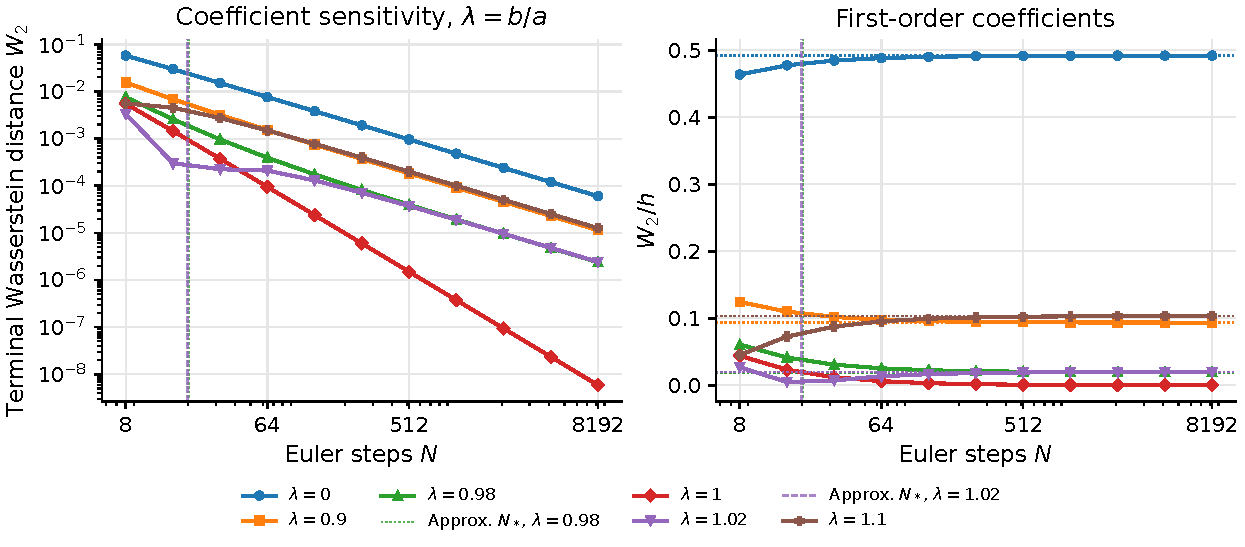
\includegraphics[width=\linewidth]{../results/figures/gaussian_sensitivity.pdf}
\caption{A fixed rotation mismatch gives first-order Euler distribution error for these Gaussian cases, with the parameters of Figure~\ref{fig:gaussian}. Each curve keeps $\lambda=b/a$ fixed as the grid is refined. The right panel shows error divided by $h$. For $\lambda\ne1$, this ratio tends to the positive value $|1-\lambda^2|c_0^{\rm G}$ shown by a horizontal dotted line. Section~\ref{sec:limits} defines $c_0^{\rm G}$. With matched rotation $\lambda=1$, the limit is zero. Vertical lines near $N=20$ estimate where the first- and second-order terms have similar size for $\lambda=0.98$ (dotted) and $1.02$ (dashed). Markers distinguish the error curves from their limits.}
\label{fig:sensitivity}
\end{figure}
\FloatBarrier

\subsection{Affine changes of coordinates, product distributions, and a dimension restriction}
\label{app:extensions}

A fixed affine change of coordinates can give distributions that are not radial in the original coordinates. For $\mathcal T(x)=d_{\rm aff}+Gx$ with $G$ invertible, set $\widetilde u(t,y)=Gu(t,G^{-1}(y-d_{\rm aff}))$ and $\widetilde p_t=\mathcal T_\#p_t$. Substitution into the differential equation and Euler update gives
\[
 \widetilde F_{s,t}\circ\mathcal T=\mathcal T\circ F_{s,t},\qquad
 \widetilde E_{t,h}\circ\mathcal T=\mathcal T\circ E_{t,h}.
\]
The transformed acceleration is $\widetilde{\acc}_t(\mathcal T(x))=G\acc_t(x)$. For every compact smooth test $\phi$,
\[
 \int\nabla\phi(y)\cdot\widetilde{\acc}_t(y)\,\widetilde p_t(\dd y)
 =\int\nabla(\phi\circ\mathcal T)(x)\cdot\acc_t(x)\,p_t(\dd x)=0.
\]
Because the affine map is invertible, $\phi\circ\mathcal T$ has compact support. The map also preserves the required smoothness, Lipschitz, growth, and moment assumptions, with different constants.

Write $s_{\min}(G)>0$ for the smallest singular value and $\|G\|_{\rm op}$ for the operator norm. Push forward any coupling to obtain the upper bound below, then apply that bound to $\mathcal T^{-1}$ to obtain the lower bound:
\[
 s_{\min}(G)W_2(\mu,\nu)
 \le W_2(\mathcal T_\#\mu,\mathcal T_\#\nu)
 \le\|G\|_{\rm op}W_2(\mu,\nu).
\]
Differences between particles from the same starting point satisfy the same norm bounds. These factors are fixed, so the positive limits in Theorem~\ref{thm:nonlinear} give orders $\Theta(h)$ and $\Theta(h^2)$ after the change of coordinates as well. The corrected distribution error is therefore smaller on sufficiently fine uniform grids. The estimates do not give exact coefficients or improvement on every grid. For example, $G=\operatorname{diag}(2,1)$ gives an elliptical mixture whose shape changes with time. This example is still an affine image of the symmetric one. Since $G(Du_0)G^{-1}$ need not be symmetric, the transformed base field need not minimize kinetic action.

We can also add independent stationary coordinates. This gives the product path $p_t\otimes\nu_{\rm stat}$ with field $(u_i,0)$, where $\nu_{\rm stat}$ has finite second moment. Projection onto the moving coordinates shows that the product $W_2$ is at least the original distance. Pairing each stationary coordinate with itself achieves this lower bound. Thus
\[
 W_2(\widehat p_k^i\otimes \nu_{\rm stat},p_{t_k}\otimes \nu_{\rm stat})
 =W_2(\widehat p_k^i,p_{t_k}).
\]
The stationary coordinates also leave particle error unchanged. Taking $\nu_{\rm stat}$ on $\R$ gives a three-dimensional example, and adding more coordinates gives examples in every dimension $d\ge2$. Independent products of moving planar examples also retain both error orders and strict improvement, since their squared $W_2$ distances add across components.

A dimension restriction applies if a tangent correction must cancel radial acceleration everywhere on a sphere while keeping the given radial coefficient. For $u(x)=\alpha(r)x+V(x)$ with $x\cdot V(x)=0$, differentiation in direction $V$ gives $x\cdot(DV)V=-\|V\|^2$. Differentiating the remaining acceleration terms yields
\[
 x\cdot\acc_u(x)=P(r)r^2-\|V(x)\|^2.
\]
Cancellation requires $\|V(x)\|^2=P(r)r^2>0$ at every point of each positive-radius sphere. In odd-dimensional space, such a sphere has even surface dimension, and the hairy-ball theorem requires every continuous tangent field to vanish somewhere~\citep[Theorem~2.28]{hatcher2002algebraic}. This rules out a tangent correction with the required cancellation at every point. Other fields can still have zero weighted divergence of acceleration, as the example with stationary coordinates shows.

\section{Robustness to an acceleration residual}
\label{app:robustness}

When only part of acceleration preserves the distribution, we shift the starting point along that part. The remaining acceleration contributes a first-order term to the global error bound. Proposition~\ref{prop:robustness} requires a bound on this remainder at every time, including Euler's evaluation times.

\begin{quote}
\textbf{Proposition~\ref{prop:robustness}, restated.}
Let $T>0$, $p_0\in\mathcal P_2$, and $p_t=(F_{0,t})_\#p_0$. Suppose $u$ is $C^2$ on a neighborhood of $[0,T]\times\R^d$, globally Lipschitz in space with constant $L$, and bounded at zero uniformly in time. Define $\acc$ and $\jerk$ as in Appendix~\ref{app:general}, and assume $C_j=\sup_t\|\jerk_t\|_{L^2(p_t)}<\infty$. Suppose
\[
 \acc_t=w_t+g_t,
 \qquad C_{w,2}=\sup_t\|w_t\|_{L^2(p_t)}<\infty,
 \qquad\sup_t\|g_t\|_{L^2(p_t)}\le\varepsilon.
\]
For each time, require $w_t\in C^1$ to be globally Lipschitz with a common constant $L_w$ and to have zero weighted divergence under $p_t$. With Euler's method and the grid defined above, put
$C_w=C_j/6+LC_{w,2}/2+TL_wC_{w,2}/8$. Then
\begin{equation}
 \max_k W_2(\widehat p_k,p_{t_k})
 \le e^{LT}\left(C_w\sum_jh_j^3+
                  \frac\varepsilon2\sum_jh_j^2\right)
 \le e^{LT}T\left(C_wH^2+\frac\varepsilon2H\right).
 \label{eq:robustness-full}
\end{equation}
\end{quote}
\begin{proof}[Proof of Proposition~\ref{prop:robustness}]
\label{proof:robustness}
For $X\sim p_t$, hold physical time fixed and follow the flow of $w_t$ for auxiliary duration $h^2/2$. This motion preserves $p_t$. The shift has $L^2$ norm at most $C_{w,2}h^2/2$ and remainder at most $L_wC_{w,2}h^4/8$ after its linear term. It supplies the $w_t$ part of the exact second-order displacement $h^2(w_t+g_t)/2$. The residual and exact-flow remainder stay in the error. The paired outputs therefore have root mean squared distance at most
\[
 \frac{C_j}{6}h^3+\frac{LC_{w,2}}{2}h^3+\frac{L_wC_{w,2}}{8}h^4
 +\frac\varepsilon2h^2.
\]
The Lipschitz estimate from the main proof bounds how much later Euler steps increase each error. Summing these contributions and using $\sum_jh_j^3\le TH^2$ and $\sum_jh_j^2\le TH$ proves the result.
\end{proof}

A time-dependent residual contributes $\frac12\sum_jh_j^2\varepsilon_{t_j}$. A bound on its time integral cannot control this sum, because the residual may be large at Euler's evaluation times. A small density-weighted divergence norm also need not give the required $L^2$ decomposition. Weighted $L^2$ projection separates acceleration into a part with zero weighted divergence and a remainder. This controls the norm, but it does not give the global Lipschitz bound required for the part that preserves the distribution.

The proposition bounds discretization error relative to the exact probability path of the approximate field. That path may differ from the intended path, so we must also estimate the error between the two paths. At the terminal time,
\[
 W_2(\widehat p_T^{\mathrm{approx}},p_T)
 \le W_2(\widehat p_T^{\mathrm{approx}},p_T^{\mathrm{approx}})
       +W_2(p_T^{\mathrm{approx}},p_T).
\]

\section{Dependence on the numerical solver}
\label{app:solver}

Euler and Heun require different rotations to cancel their leading Gaussian distribution errors. We first compare their expansions at a common step length, then pair two corrected Euler steps with one base-field Heun step to compare equal numbers of field evaluations.

\begin{proposition}[Euler and Heun for a fixed Gaussian rotation]
\label{prop:solver-dependence}
Let $T>0$, $a>0$, and let $\Sigma_0=C_0C_0^\top$ be positive definite in even dimension. Let $J^\top=-J$, $J^\top J=I$, $\Omega=C_0JC_0^{-1}$, $m_t=m_0+t\xi$, and $p_t=\mathcal N(m_t,e^{2at}\Sigma_0)$. For a fixed real $b$, use
\[
 v_b(t,x)=\xi+(aI+b\Omega)(x-m_t).
\]
On uniform grids with $h=T/N$, Euler satisfies
\begin{equation}
 W_2(\widehat p_N^{\mathrm E,b},p_T)
 =\sqrt{\tr\Sigma_0}e^{aT}\frac{T|a^2-b^2|}{2}h+O(h^2).
 \label{eq:gaussian-fixed-sensitivity}
\end{equation}
Define Heun by
\[
 x^*=x+hv_b(t,x),\qquad
 x^+=x+\frac h2[v_b(t,x)+v_b(t+h,x^*)].
\]
Its terminal error satisfies
\begin{equation}
 W_2(\widehat p_N^{\mathrm H,b},p_T)
 =\sqrt{\tr\Sigma_0}e^{aT}
       \frac{T|a(a^2-3b^2)|}{6}h^2+O(h^3).
 \label{eq:heun-leading-error}
\end{equation}
In particular, Heun's positive leading constant at $b=a$ is twice its constant at $b=0$. The leading Heun term cancels at $b=\pm a/\sqrt3$, giving an $O(h^3)$ bound in this family.
\end{proposition}

\paragraph{Proof idea.}
In centered whitened coordinates, each solver acts as a polynomial in $a+\mathrm i b$. The real part of the polynomial's logarithm gives the numerical log scale. We use this scale to calculate Gaussian distribution error.

\begin{proof}
The exact centered flow $e^{at}C_0e^{btJ}C_0^{-1}$ has the same covariance and mean for every $b$. Both solvers reproduce the affine mean exactly. For the centered whitened operator $B=aI+bJ$, Euler applies $I+hB$, while Heun applies $I+hB+h^2B^2/2$.

A matrix $cI+dJ$ multiplies whitened covariance by $c^2+d^2$, the squared complex modulus of $c+\mathrm i d$. Thus scalar complex calculations give the distribution error. With $w=h(a+\mathrm i b)$, the exact, Euler, and Heun scale factors are $e^{ah}$, $|1+w|$, and $|1+w+w^2/2|$. Writing $\Delta^{\mathrm{log}}$ for exact minus numerical log scale after $N$ steps, we use
\begin{align*}
 \log(1+w)&=w-\tfrac12w^2+O(w^3),\\
 \log(1+w+w^2/2)&=w-\tfrac16w^3+O(w^4).
\end{align*}
Taking real parts and multiplying by $N=T/h$ shows that
\[
 \Delta^{\mathrm{log}}_{\mathrm E}=\frac T2(a^2-b^2)h+O(h^2),\qquad
 \Delta^{\mathrm{log}}_{\mathrm H}=\frac T6a(a^2-3b^2)h^2+O(h^3).
\]
By the Gaussian scale identity,
$W_2=\sqrt{\tr\Sigma_0}e^{aT}|1-e^{-\Delta^{\mathrm{log}}}|$.
Substitution gives the stated errors. For Heun, the absolute cubic coefficients are $a^3/6$ at $b=0$ and $a^3/3$ at $b=a$, so Euler's correction doubles Heun's leading coefficient. The cubic coefficient instead vanishes at $b^2=a^2/3$.
\end{proof}

Euler's leading term cancels at $b=\pm a$, or only at $b=a$ if $b\ge0$ is required. For fixed $\delta_b$ with $b=a(1+\delta_b)$ and $b^2\ne a^2$, Eq.~\eqref{eq:gaussian-fixed-sensitivity} gives the positive first-order coefficient $\sqrt{\tr\Sigma_0}e^{aT}Ta^2|2\delta_b+\delta_b^2|/2$. Appendix~\ref{app:nonlinear-sensitivity} gives the corresponding result for nonlinear fields.

For this family, applying the matrix exponential of the full constant centered operator gives the exact solution. An exponential integrator that splits or approximates this operator needs a separate error analysis.

\begin{figure}[ht]
\centering
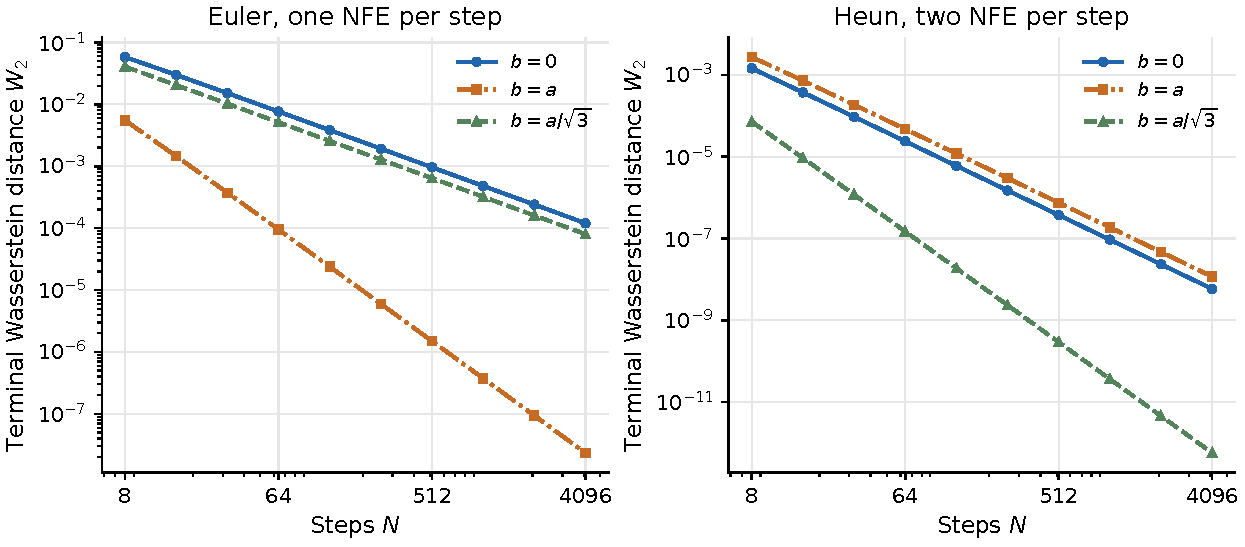
\includegraphics[width=\linewidth]{../results/figures/solver_dependence.pdf}
\caption{Euler and Heun require different rotations to cancel their leading distribution errors. Both methods use the Gaussian path and parameters of Figure~\ref{fig:gaussian}, with the same number of uniform steps. Rotation $b=a$ improves Euler but doubles Heun's leading coefficient relative to $b=0$. For Heun, $b=a/\sqrt3$ cancels the second-order term. Heun uses two evaluations per step, so the methods have unequal NFE here. Figure~\ref{fig:equal-evaluation}, Table~\ref{tab:few-evaluations}, and Table~\ref{tab:gaussian-higher-order} compare equal NFE.}
\label{fig:solver}
\end{figure}
\FloatBarrier

\subsection{Equal NFE for corrected Euler and base-field Heun}
\label{app:equal-evaluation}

\begin{proof}[Proof of Proposition~\ref{prop:equal-nfe}]
Let $N$ be even and $h=T/N$. In centered whitened coordinates, two corrected Euler steps of length $h$ have scale multiplier
\[
 \left(\sqrt{1+2ah+2a^2h^2}\right)^2
 =1+a(2h)+\tfrac12a^2(2h)^2.
\]
This is also the positive scale multiplier of one base-field Heun step of length $2h$. Both methods reproduce the affine mean. Their covariances match, so their Gaussian distributions are identical at every shared node. Euler uses one evaluation per step and Heun uses two, giving $N$ evaluations for each method on $[0,T]$. The same argument applies when consecutive Euler steps come in equal-length pairs on an otherwise nonuniform grid.
\end{proof}

\subsection{Corrected Heun and base-field RK3 at equal NFE}
\label{app:heun-rk3}

At $b=a/\sqrt3$, Heun's second-order distribution term cancels and the remaining third-order coefficient is positive. We calculate this coefficient and compare Heun with base-field RK3 using the same number of evaluations. Put $\zeta=a+\mathrm i b$, $R_2(w)=1+w+w^2/2$, and $C_\Sigma=\sqrt{\tr\Sigma_0}e^{aT}$. After $n=T/h$ uniform steps, Heun's errors are exactly
\begin{align}
 W_2^{\mathrm H,b}&=\sqrt{\tr\Sigma_0}\left|e^{aT}-|R_2(h\zeta)|^n\right|,\\
 e_{\mathrm p}^{\mathrm H,b}&=\sqrt{\tr\Sigma_0}\left|R_2(h\zeta)^n-e^{T\zeta}\right|.
 \label{eq:heun-exact-particle}
\end{align}
Here $e_{\mathrm p}$ is the root mean squared particle error from Section~\ref{sec:setup}. The formulas also apply to elliptical covariance, since a map difference $cI+dJ$ in transformed coordinates contributes covariance $(c^2+d^2)\Sigma_0$ in the original coordinates.

Since $\log R_2(w)=w-w^3/6+w^4/8+O(w^5)$, the choice $b=a/\sqrt3$ cancels the real cubic term. The remaining coefficients satisfy $\operatorname{Re}\zeta^4=-8a^4/9$ and $\operatorname{Im}\zeta^3=8a^3/(3\sqrt3)$. Thus
\begin{align}
 W_2^{\mathrm H,a/\sqrt3}&=C_\Sigma\frac{a^4T}{9}h^3+O(h^4),\\
 e_{\mathrm p}^{\mathrm H,a/\sqrt3}&=C_\Sigma\frac{4a^3T}{9\sqrt3}h^2+O(h^3).
 \label{eq:heun-attained-orders}
\end{align}
Both coefficients are positive, so distribution error is third order and particle error is second order.

For comparison, Kutta's three-stage, third-order Runge--Kutta method uses
\[
 k_1=v(t,x),\quad k_2=v(t+s/2,x+sk_1/2),\quad
 k_3=v(t+s,x-sk_1+2sk_2),\quad
 x^+=x+s(k_1+4k_2+k_3)/6.
\]
On the base field $v_0$, its centered scale factor is $R_3(as)=1+as+(as)^2/2+(as)^3/6$. Because $\log R_3(z)=z-z^4/24+O(z^5)$,
\[
 W_2^{\mathrm{RK3},0}=C_\Sigma\frac{a^4T}{24}s^3+O(s^4).
\]
The base-field Runge--Kutta map is a positive scalar dilation. Pairing particles from the same starting point is therefore optimal, so particle error equals distribution error.

For an evaluation count $N$ divisible by six, corrected Heun takes $N/2$ steps and base RK3 takes $N/3$. Substitution of $h=2T/N$ and $s=3T/N$ into the two error expansions proves
\[
 \lim_{N\to\infty}\frac{W_2^{\mathrm H,a/\sqrt3}}{W_2^{\mathrm{RK3},0}}=\frac{64}{81}.
\]
At the finite evaluation counts in Table~\ref{tab:gaussian-higher-order}, corrected Heun has 18.0--20.9\% smaller distribution error, while its particle error is larger.

\begin{table}[ht]
\centering
\begin{tabular}{rccc}
\toprule
NFE & \shortstack{Corrected field\\Heun $W_2$} & \shortstack{Base field, RK3\\$W_2$ and particle error} & \shortstack{Corrected field\\Heun particle error} \\
\midrule
12 & $1.677\times10^{-4}$ & $2.046\times10^{-4}$ & $3.904\times10^{-3}$ \\
48 & $2.790\times10^{-6}$ & $3.497\times10^{-6}$ & $2.581\times10^{-4}$ \\
192 & $4.426\times10^{-8}$ & $5.588\times10^{-8}$ & $1.636\times10^{-5}$ \\
384 & $5.547\times10^{-9}$ & $7.011\times10^{-9}$ & $4.100\times10^{-6}$ \\
\bottomrule
\end{tabular}

\caption{Corrected Heun has smaller distribution error but larger particle error than base-field RK3 at the listed evaluation counts. The parameters are those of Figure~\ref{fig:gaussian}, with $b=a/\sqrt3$ for Heun and $b=0$ for RK3. Both fields stay fixed as NFE increases.}
\label{tab:gaussian-higher-order}
\end{table}
\FloatBarrier

\section{Restrictions on the mean, second moment, and action}
\label{app:obstruction}

The acceleration condition requires the mean to move at constant velocity. It also determines kinetic action from the path's second moment. If a path fails these restrictions, no field in the stated class can satisfy the acceleration condition. Other ways to improve numerical accuracy may still be possible.

For Proposition~\ref{prop:obstruction}, let $X_t$ follow a global flow on $[0,T]$. Assume its trajectories and their first two derivatives are continuous, with $\dot X_t=u_t(X_t)$ and $\ddot X_t=\acc_t(X_t)$. One sufficient condition for the differentiations below is
\begin{equation}
 \E\sup_{0\le t\le T}
 [\|X_t\|^2+\|u_t(X_t)\|^2+\|\acc_t(X_t)\|^2]<\infty.
 \label{eq:moment-differentiation-assumption}
\end{equation}
More generally, require that the second moment can be differentiated twice under the expectation and that $u_t,\acc_t\in L^2(p_t)$. If $\acc_t$ has zero weighted divergence under the current distribution, then
\begin{equation}
 M''(t)=2\E\|u_t(X_t)\|^2,
 \qquad M(t)=\E\|X_t\|^2.
 \label{eq:moment-obstruction-full}
\end{equation}

\paragraph{Proof idea.}
The second derivative of the second moment contains kinetic energy and an acceleration term. To remove the acceleration term, we approximate squared distance by compactly supported tests and use zero weighted divergence. The remaining identity determines energy. This energy must be at least the infimum over fields satisfying the given continuity equation.

\begin{proof}[Proof of Proposition~\ref{prop:obstruction}]
Differentiating twice shows that
\[
 M''(t)=2\E\|u_t(X_t)\|^2+2\E[X_t\cdot\acc_t(X_t)].
\]
Condition~\eqref{eq:moment-differentiation-assumption} gives an integrable derivative bound, so dominated convergence and Cauchy--Schwarz justify differentiation under expectation. To test zero weighted divergence, replace squared distance by $\chi_n(x)\|x\|^2/2$, using the smooth compact cutoffs of Appendix~\ref{app:projection}. The gradient converges to $x$ in $L^2(p_t)$ as the second-moment tail vanishes. Since $\acc_t\in L^2(p_t)$, passage to the limit gives $\E[X_t\cdot\acc_t(X_t)]=0$ and proves Eq.~\eqref{eq:moment-obstruction-full}.

Let $K_{\min}(t)$ be the infimum of kinetic energy over fields satisfying the weak continuity equation for the path at time $t$. These competitors need not satisfy the acceleration condition. The chosen field has energy at least this infimum, giving $M''(t)\ge2K_{\min}(t)$. For a stationary distribution, $M''=0$ forces the field to vanish $p_t$-almost everywhere, or everywhere if the field is continuous and the density is positive throughout space.

For a centered radial dilation $p_t=(g(t)I)_\#p_0$, let $p_0$ be rotationally invariant and suppose $g>0$ is $C^2$ and $M_0=\int\|x\|^2p_0(\dd x)>0$ is finite. The base field is the gradient $v_t(x)=(g'/g)x$. The cutoff argument in Appendix~\ref{app:projection} places this gradient in the required closure. The projection identity then implies
\[
 K_{\min}(t)=M_0g'(t)^2,\qquad
 M''(t)=2M_0[g'(t)^2+g(t)g''(t)].
\]
When $g''(t)<0$, the necessary energy inequality fails. No field with the stated regularity and finite energy can then have zero weighted divergence of acceleration. For a scaling path that does admit such a field, its kinetic energy above that of the base field must equal $M_0g(t)g''(t)$.
\end{proof}

When $g''=0$, extra energy must be zero and the base acceleration is zero. If $g''>0$, an even-dimensional radial distribution can satisfy this necessary condition through
\[
 u(t,x)=\frac{g'}g x+b(t)Jx,\qquad b(t)^2=\frac{g''}g,
 \quad J^\top=-J,\quad J^\top J=I.
\]
Provided the square root has the required regularity, differentiation gives $\acc_u=[b'+2(g'/g)b]Jx$, which has zero weighted divergence for a radial distribution. Zeros of $g''$ require an additional check of square-root smoothness. Terminal accuracy can still occur when the local acceleration condition fails, through cancellation across steps (Appendix~\ref{app:local}).

\paragraph{Independent Gaussian interpolation at the midpoint.}
Independent interpolation pairs can have different kinetic energy from their conditional-mean field. For independent two-dimensional standard Gaussians $X_0,X_1$, let $X_t=(1-t)X_0+tX_1$. At $t=1/2$, the position depends on $X_0+X_1$, which is independent of $X_1-X_0$. The conditional mean velocity is therefore zero, although $\E\|X_1-X_0\|^2=4$. The path remains nonstationary, with variance decreasing before the midpoint and increasing afterwards.

\begin{proof}[Proof of Corollary~\ref{cor:mean-action}]
The same integrability assumption also lets us differentiate the mean twice under expectation. By Condition~\eqref{eq:moment-differentiation-assumption},
\[
 m'(t)=\E u_t(X_t),\qquad m''(t)=\E\acc_t(X_t).
\]
To evaluate the acceleration expectation, choose a smooth compact cutoff $\chi$ equal to one near the origin and put $\chi_n(x)=\chi(x/n)$. Testing Eq.~\eqref{eq:flux-null} with $\phi_n(x)=\chi_n(x)x_j$ gives gradients converging pointwise to $e_j$, with a bound independent of $n$. Since $\acc_t\in L^2(p_t)\subset L^1(p_t)$, dominated convergence gives $\E\acc_{t,j}(X_t)=0$. Hence $m''(t)=0$ and $m(t)=m(0)+t\E u_0(X_0)$.

Integrating Eq.~\eqref{eq:moment-obstruction-full} gives the action identity in Eq.~\eqref{eq:mean-action}. The moment assumption makes $M$ twice continuously differentiable, with endpoint derivatives taken from inside the interval. Thus the given path determines both the energy at each time and the total action for every field in this class.

If a gradient base field $v^\nabla$ generates the given path and satisfies the conditions in Section~\ref{sec:path-restrictions}, Eq.~\eqref{eq:projection} gives
\[
 \int_0^T\|u_t-v_t^\nabla\|_{L^2(p_t)}^2\dd t
 =\tfrac12\bigl[M'(T)-M'(0)\bigr]-\cA_T(v^\nabla).
\]
The path therefore determines the additional action within this class. The identity alone does not show that such a field exists.

The assumptions of Theorem~\ref{thm:distribution_order} also imply the required moment condition. With $U=\sup_t\|u(t,0)\|$, Gronwall's inequality gives
\[
 \sup_{0\le t\le T}\|X_t\|\le (\|X_0\|+TU)e^{LT}.
\]
Continuity gives $C_{a,0}=\sup_t\|\acc_t(0)\|<\infty$, and the common Lipschitz bounds give $\|u_t(X_t)\|\le U+L\|X_t\|$ and $\|\acc_t(X_t)\|\le C_{a,0}+L_a\|X_t\|$. Each squared time supremum is therefore bounded by $C(1+\|X_0\|^2)$ for finite $C$, which is integrable under the source second moment.
\end{proof}

\section{Minimum action among fields with the same path}
\label{app:projection}

We compare actions by using a gradient base field that can be approximated in mean square by compactly supported gradients. Such a field is orthogonal to every correction that preserves the probability path. For compactly supported potentials, zero weighted divergence gives this orthogonality directly. For the unbounded Gaussian and radial potentials, we use cutoff approximation to obtain the same result in mean square.

We use $\cV(p)$ for fields that are jointly continuous, have finite action, and are locally Lipschitz in space uniformly on compact time-space sets. Their flows must exist on $[0,T]$ and generate the given path. The action identity also holds for the larger class of finite-action fields satisfying the same weak continuity equation.

At each time, define the space of gradients and their mean square limits by
\[
 \mathcal G_t=\overline{\{\nabla\psi:\psi\in C_c^\infty(\mathbb R^d)\}}
 ^{L^2(p_t)}.
\]
Suppose $v_t\in\mathcal G_t$ for almost every time and $v$ has finite action. Let $r$ have finite action with $\nabla\!\cdot(p_tr_t)=0$ distributionally for almost every time. For every smooth compactly supported potential, $\mathbb E_{p_t}[r_t\cdot\nabla\psi]=0$. By continuity of the inner product in weighted $L^2(p_t)$, we also have $\mathbb E_{p_t}[r_t\cdot v_t]=0$. The cross term is therefore zero when we expand squared velocity and integrate, proving Eq.~\eqref{eq:projection}. Equal action requires $r=0$ almost everywhere under $dt\,p_t(dx)$, which means almost surely in position for almost every time. To obtain equality everywhere, we need the continuity and positivity argument below. Differences between fields satisfying the same continuity equation have the required zero weighted divergence. The existence of their particle flows is a separate requirement.

For the gradient fields used here, a finite second moment is enough to justify approximation by compactly supported gradients. Let $v_t(x)=\nabla\varphi_t(x)$, where
$\varphi_t$ has at most quadratic growth and its gradient has at most
linear growth, uniformly on the fixed time interval. Choose a smooth cutoff function
$\chi_n$ that is one on the radius-$n$ ball, zero outside the radius-$2n$
ball, and has $\|\nabla\chi_n\|\le C/n$. Then
\[
 \nabla(\chi_n\varphi_t)-\nabla\varphi_t
 =(\chi_n-1)\nabla\varphi_t+\varphi_t\nabla\chi_n.
\]
The squared approximation error is bounded by a constant times $\mathbb E_{p_t}[(1+\|X\|^2)\mathbf1_{\{\|X\|>n\}}]$, which vanishes by the finite second moment. For radial dilation, $\|X_t\|=g_t\|X_0\|$ with bounded $g_t$ gives one integrable tail bound for all times. The nonlinear path satisfies the same requirement through $\|X_t\|\le e^{(a+\eta)T}\|X_0\|$ in Eq.~\eqref{eq:radial-flow-growth}. Scaling and translating a fixed Gaussian gives the corresponding bound for the Gaussian path. Compactly supported gradients therefore converge in mean square both at each time and after time integration.

When every $p_t$ has positive density throughout space, equal action in $\cV(p)$ implies equality everywhere. A continuous difference nonzero at one point stays nonzero on an open time-space neighborhood. Every spatial ball in that neighborhood has positive $p_t$ mass, contradicting almost-everywhere equality under the path. The Gaussian path therefore has a unique minimizer in this continuous class.

\subsection{Gradient fields under the acceleration condition}
\label{app:gradient}
Under all assumptions of Theorem~\ref{thm:distribution_order}, suppose each $u_t$ is a gradient on $\R^d$. We prove that $\acc_t=0$ $p_t$-almost everywhere and that, for $p_0$-almost every start, Euler's method is exact on every finite increasing grid.

\begin{proof}[Proof of Proposition~\ref{prop:gradient-straight}]
\label{proof:gradient-straight}
A gradient velocity has a symmetric spatial Jacobian, so material acceleration is also a gradient. The growth bounds let us approximate acceleration by compactly supported gradients in the weighted norm. The acceleration condition makes acceleration orthogonal to all such gradients, so its norm must be zero.

Choose the normalized potential
$\psi(t,x)=\int_0^1 u(t,sx)\cdot x\dd s$.
Because $u_t$ is a gradient, $\nabla_x\psi=u_t$. The $C^2$ regularity of $u$ lets us differentiate in time and space. Symmetry of $D_xu_t$ then implies
\[
 \acc_t=\nabla q_{\rm acc,t},\qquad
 q_{\rm acc,t}=\partial_t\psi_t+\tfrac12\|\nabla\psi_t\|^2.
\]
Subtract $q_{\rm acc,t}(0)$ from this potential. With
$C_{a,0}=\sup_{t\in[0,T]}\|\acc_t(0)\|<\infty$, the common Lipschitz bound implies
\[
 |q_{\rm acc,t}(x)|\le C_{a,0}\|x\|+\tfrac12L_a\|x\|^2,
 \qquad \|\nabla q_{\rm acc,t}(x)\|\le C_{a,0}+L_a\|x\|.
\]
The growth bounds place $\acc_t$ in $\mathcal G_t$ by cutoff approximation. If the cutoff potentials are not smooth enough for the tests, convolution gives smooth compactly supported potentials whose gradients converge uniformly on a fixed compact set, hence in $L^2(p_t)$. Zero weighted divergence also makes $\acc_t$ orthogonal to $\mathcal G_t$, so
\[
 \|\acc_t\|_{L^2(p_t)}^2=0.
\]

At each fixed time, acceleration is zero almost everywhere. We need this conclusion along complete trajectories. Choose a countable dense set of times and intersect their full-probability sets of starting points. This intersection still has full probability. By continuity of $t\mapsto\acc_t(X_t)$, acceleration is zero at every time along each selected trajectory. Hence $X_t=X_0+t u_0(X_0)$ and $u_t(X_t)=u_0(X_0)$. Each Euler update from an exact point uses this constant velocity and reaches the next exact point. Euler is therefore exact on every finite increasing grid for the same set of starts.
\end{proof}

\section{Regular displacement interpolation}
\label{app:displacement}


Regular displacement interpolation moves each source point to its target at constant velocity along a straight line. Euler follows these trajectories exactly. Under the assumptions below, the field also minimizes action. \citet[Remark~7]{tao2026strain} note exactness on straight trajectories. The proposition gives sufficient assumptions on the map and proves exactness at successive grid points.

\begin{proposition}[Euler exactness on regular displacement interpolation]
\label{prop:displacement-euler}
Let $T>0$ and let $p_0$ be absolutely continuous with a finite second moment.
Let $\mathcal Q=\nabla\Phi_{\rm OT}:\mathbb R^d\to\mathbb R^d$, where
$\Phi_{\rm OT}\in C^2$, and suppose
\[
 0<\ell_- I\preceq D\mathcal Q(x)\preceq\ell_+ I
 \qquad\text{for all }x
\]
for fixed finite constants $\ell_-$ and $\ell_+$.
Define
\[
 \mathcal T_t(x)=(1-t/T)x+(t/T)\mathcal Q(x),\qquad
 p_t=(\mathcal T_t)_\#p_0,
\]
and define the field by
\[
 u(t,\mathcal T_t(x))=\frac{\mathcal Q(x)-x}{T}.
\]
The maps $\mathcal T_t$ are global diffeomorphisms, which means that they are continuously differentiable bijections with continuously differentiable inverses. The field is jointly continuous,
globally Lipschitz in space, and has linear growth. Its trajectories are
$X_t=\mathcal T_t(X_0)$.
On every finite increasing grid, Euler's method satisfies
\[
 \widehat X_k=\mathcal T_{t_k}(X_0)
\]
for every initial point. It is therefore exact for particles and their distributions at the grid points.

The map $\mathcal Q$ is the quadratic-cost optimal map from $p_0$ to
$p_T$. The displayed path is its displacement interpolation, and
\[
 \mathcal A_T(u)=\frac{W_2^2(p_0,p_T)}{T}.
\]
The field also minimizes action among finite-action fields satisfying this
fixed continuity equation, up to $dt\,p_t(dx)$-almost-everywhere equality.
\end{proposition}

\begin{proof}
The interpolating maps need global inverses to define the field at every position. With $s=t/T$, the symmetric derivative $D\mathcal T_t=(1-s)I+sD\mathcal Q$ has eigenvalues between $\min(1,\ell_-)$ and $\max(1,\ell_+)$. The lower bound gives strong monotonicity and injectivity, as well as properness, meaning that inverse images of compact sets are compact. The inverse function theorem makes the image open, while properness makes it closed. Since the image is nonempty and $\mathbb R^d$ is connected, the map is onto and has a global differentiable inverse. The uniform derivative bounds and field formula give the stated continuity, spatial Lipschitz continuity, and linear growth.

Each trajectory is affine in time. In particular,
\[
 \mathcal T_{t+h}(x)=\mathcal T_t(x)+h\frac{\mathcal Q(x)-x}{T}.
\]
If Euler reaches the exact point at $t_k$, its next evaluation gives the same constant particle velocity and its update reaches $\mathcal T_{t_{k+1}}(x)$. Induction proves exactness on every grid.

By the convex-gradient characterization, $\mathcal Q$ is the quadratic-cost optimal map~\citep[Section~6.2.3]{ambrosio2005gradient}. Each particle has constant velocity, giving action $\mathbb E\|\mathcal Q(X_0)-X_0\|^2/T$. Since the map is optimal, this action equals the stated Wasserstein formula.

For minimum action with the path fixed, it remains to place the velocity in the weighted gradient closure. At $y=\mathcal T_t(x)$, the spatial derivative is
\[
 D_yu(t,y)=\frac1T(D\mathcal Q(x)-I)
 \{(1-s)I+sD\mathcal Q(x)\}^{-1}.
\]
The matrices are symmetric and commute, so $D_yu$ is symmetric and $u_t$ is a gradient. Linear field growth gives at most quadratic potential growth, allowing cutoff approximation under finite second moments. If a cutoff potential is only $C^2$, convolution gives smooth potentials with uniformly convergent gradients on a compact support. Thus velocity lies in the weighted gradient closure, and the projection identity proves minimum action on the fixed path.
\end{proof}

These map assumptions are sufficient for both exactness and action minimization. Euler exactness alone needs only a well-defined field at evaluation times along constant-velocity straight paths. For a singular optimal-transport map, the existence of such a field needs a separate argument.

\section{A scaled rotated Gaussian coupling}
\label{app:fm}

We scale the rotated Gaussian pairing of \citet[Example~3.5]{liu2022marginal} to obtain the same probability path as independent Gaussian interpolation, using dependent endpoints. In even dimension, let $\sigma>0$, $J^\top=-J$, $J^\top J=I$, and $X_0\sim\mathcal N(0,I)$. With $\mathcal T_t=(1-t)I+\sigma tJ$ on $[0,1]$, each particle follows a straight line to a scaled rotation of its start. The endpoints are dependent, but $\mathcal T_t\mathcal T_t^\top=q_{\rm G}(t)I$ with $q_{\rm G}(t)=(1-t)^2+\sigma^2t^2>0$, giving the same Gaussian marginals as independent interpolation. The velocity field is
\begin{equation}
 u(t,x)=(\sigma J-I)\mathcal T_t^{-1}x
 =\frac{\sigma^2t-(1-t)}{q_{\rm G}(t)}x+\frac\sigma{q_{\rm G}(t)}Jx.
 \label{eq:fm-rotated-field}
\end{equation}
The radial term is the conditional-mean gradient velocity of independent Gaussian interpolation, while the rotation preserves each Gaussian marginal. Since $\mathcal T_{t+h}=\mathcal T_t+h(\sigma J-I)$, an Euler update from an exact point reaches the next exact point. Induction gives particle exactness on every grid, although rotation raises action above the gradient field by $d\sigma^2\int_0^1q_{\rm G}(t)^{-1}\dd t>0$.

For an anisotropic endpoint $CX_0$ with covariance $\Sigma_1=CC^\top$, this deterministic linear construction matches the independent-interpolation path exactly when $C+C^\top=0$. This follows by comparing the $t(1-t)$ covariance terms. An invertible real skew-symmetric matrix has two-dimensional blocks, so each eigenvalue of $CC^\top$ has even multiplicity. Conversely, equal eigenvalues can be paired into blocks $\sqrt\mu J$. The restriction applies only to this linear coupling class.

\section{Limits of action comparisons and evaluation schedules}
\label{app:schedules}

Our examples use fields with positive additional action. In a larger class of fields, the same numerical improvement can require arbitrarily little additional action. Euler uses the field only at its evaluation times, while action integrates squared velocity over time. A continuous correction can keep the same values at evaluation times and vanish outside short intervals around them.

For the Gaussian probability path in Appendix~\ref{app:fixed-gaussian}, fix a finite increasing grid and $a>0$. At step $j$, set
\[
 b_j=h_j^{-1}\sqrt{e^{2ah_j}-(1+ah_j)^2}.
\]
The inequality $e^{ah_j}>1+ah_j$ makes $b_j$ real and positive, with exact Euler covariance factor $(1+ah_j)^2+b_j^2h_j^2=e^{2ah_j}$. Set $b(t_j)=b_j$ at each evaluation time and extend these values by continuous functions supported in disjoint intervals of width at most $\delta$. Their sum $b_\delta$ is bounded and continuous, giving a global affine flow that preserves the Gaussian path. Shrinking the intervals keeps every Euler evaluation and output unchanged, while the added action satisfies
\[
 \tr(\Sigma_0)\int_0^T b_\delta(t)^2e^{2at}\dd t\longrightarrow0
 \quad\text{as }\delta\downarrow0.
\]
The grid is fixed and has finitely many evaluation times. The function heights are finite, so the action integral tends to zero as the total support length decreases. This gives the same numerical improvement with arbitrarily small additional action. The fields have no common bound on time derivatives.

\section{Numerical specification}
\label{app:numerics}

We calculate distances between full probability distributions, without using sample estimates. For the Gaussian examples, recursive matrix updates check the distance formulas and particle maps. For the nonlinear example, optimal radial transport gives the distances. We use independent reference calculations to check the nonlinear distances and their leading coefficients.

\subsection{Gaussian checks}

We evaluate the scalar Gaussian formulas at 80 decimal digits. We check the particle maps, covariances, and means against recursive Euler matrix updates in binary64 double precision. Each update starts from the preceding numerical result, with the mean moving at constant velocity. To calculate the Gaussian Wasserstein distance, we optimally align the covariance square roots by an orthogonal map. This avoids subtracting nearly equal trace terms. Quadrature along the exact flow gives an independent check of continuous action.

The nonuniform grid is $(0,0.04,0.17,0.43,0.72,1)$.

The Gaussian calculation uses $a=0.6$, $T=1$, and the fixed coefficients $b=0$ and $b=a$. In dimension two, the covariance is
\begin{equation}
 \Sigma_0=\begin{pmatrix}1.5&0.25\\0.25&0.75\end{pmatrix}.
 \label{eq:numerical-covariance}
\end{equation} Uniform step counts are the powers of two from one through 4096. Dimensions four and eight use $1,4,32$ uniform steps. All three dimensions also use the nonuniform grid above. For each higher dimension $d$, set $\Sigma_0=C_0C_0^\top$, where
\[
 (C_0)_{ii}=0.7+0.9\frac{i-1}{d-1},\qquad (C_0)_{i,i-1}=0.12\ (i\ge2),
\]
and all other entries vanish. For every dimension, the mean and drift components are
\[
 (m_0)_i=-0.4+\frac{i-1}{d-1},\qquad
 \xi_i=0.2-0.5\frac{i-1}{d-1}.
\]
The matrix $J$ uses consecutive two-dimensional quarter-turn blocks. We compare terminal squared distribution error, its maximum over grid points, and its sum over grid points. We also calculate error between particles from the same starting point and check the positive leading error coefficients in Appendix~\ref{app:fixed-gaussian}.

The contraction control uses $a=b=-0.6$, the stated two-dimensional covariance, and one step on $[0,1]$, with algebraic zeros recorded separately from floating-point residuals.

\subsection{Nonlinear example and reference calculations}

The nonlinear calculation uses $a=0.6$, $\eta=0.3$, $T=1$, and source $0.6\mathcal N(0,0.5^2I_2)+0.4\mathcal N(0,1.5^2I_2)$. The uniform step counts are powers of two from 8 through 4096. We also use the same unequal grid as above. For a spherical Gaussian component of scale $s$, $R_0^2/(2s^2)$ has density $e^{-z}$ on $z\ge0$. We therefore evaluate radius expectations by Gauss--Laguerre quadrature with 64, 128, or 256 nodes per component.

For the first reference calculation, we integrate log radius, angle, action, and the coefficient equations over time. We use SciPy 1.17.0's DOP853 ordinary differential equation solver, with primary relative and absolute tolerances $2\times10^{-13}$ and $2\times10^{-14}$. For an independent reference, we separate variables in the radius equation. With $r>0$, $a_+=a+\eta$, and $\ell=\log(R(T,r)/r)$, this gives the implicit equation
\[
 \frac\ell a-\frac\eta{2a a_+}
 \log\frac{a+a_+r^2e^{2\ell}}{a+a_+r^2}=T,
 \qquad aT\le\ell\le a_+T.
\]
This equation comes from integrating $1/f(r)$ between the source and terminal radii. Once we find the terminal radius, we integrate over radius to calculate angle, action, and leading coefficients. This calculation is independent of the time integration. Differentiating $\log f(R(s,r))$ gives $V(T,s;r)=f(R(T,r))/f(R(s,r))$ for $r>0$, so
\[
 \mathcal C_i(T,r)=f(R(T,r))\int_r^{R(T,r)}\frac{d_i(v)}{f(v)^2}\dd v.
\]
To separate quadrature error from reference error, we first increase the number of nodes with tolerances fixed. We then tighten the tolerances with the number of nodes fixed. The supplementary code includes all tolerances and comparison criteria.

We also compare independent particle updates in Cartesian and radius-angle coordinates, using source radii $(0.07,0.4,1,3,8)$ and angles $(0,0.3,1,2.1,4)$.

\subsection{Solver, sensitivity, and interpolation checks}

The solver calculations use $b=0$, $b=a$, and $b=a/\sqrt3$ on the same grids. We check the scalar stability factors against separate matrix updates. To study Euler's sensitivity, we use fixed ratios $b/a\in\{0,0.9,0.98,1,1.02,1.1\}$. The interpolation calculation uses $\sigma=1.5$. Its corrected field has zero error algebraically, and we record floating-point residuals separately. These computations check the numerical evaluation of the formulas. The proofs give the convergence orders and strict comparisons.


\subsection{Equal NFE}

For the nonlinear equal-NFE comparison, we keep the same source and coefficients and use $N\in\{2^j:j=1,\ldots,12\}$ evaluations. Euler takes $N$ uniform steps, while base-field Heun takes $N/2$. We calculate distances using 128 Gauss--Laguerre nodes per component and compare them with results from 64 and 256 nodes. All methods use the implicit exact-radius reference. We check this reference independently by time integration at relative tolerance $2.5\times10^{-14}$ and absolute tolerance $3\times10^{-15}$.

For base-field Heun, put $f(r)=\alpha(r)r$ and let $s=2T/N$. One radius step is
\[
 H_s(r)=r+\tfrac{s}{2}\{f(r)+f(r+sf(r))\}.
\]
Since $f'>0$, its derivative is
$1+\tfrac{s}{2}\{f'(r)+f'(r+sf(r))[1+sf'(r)]\}>0$.
The derivative is positive, so the radius map is increasing. The update also preserves angle. Pairing particles from the same starting point therefore matches angles and ordered radii. This pairing is optimal, so particle error equals $W_2$. We check all three methods with separate Cartesian updates. The smaller measured distribution error of corrected Euler applies to this source and these parameters.

Increasing quadrature from 128 to 256 nodes changes the errors by less than $1.8\times10^{-7}$ relatively, while the independent reference discrepancy is below $2.6\times10^{-8}$ of the corresponding numerical error.

The Gaussian Heun--RK3 comparison uses the parameters of Figure~\ref{fig:gaussian} at $12,48,192,384$ field evaluations. We evaluate the complex polynomials at 50 and 80 decimal digits and check them against independent matrix-stage recurrences at 70 and 100 digits. The extra precision controls error from subtracting nearby values in the distance calculation.

\subsection{Measured errors and refinement results}

Table~\ref{tab:nonlinear-results} gives the errors on the finest grid and order estimates $\log_2(e_{2048}/e_{4096})$, where $e_N$ is error after $N$ steps. We calculate the leading coefficients from independent radius integrals, without fitting the error curves. The primary calculation uses \NonlinearQuadratureOrder\ nodes per mixture component. Increasing this to 256 changes every reported terminal error, action, and coefficient by less than $8\times10^{-8}$ relatively. The largest reference discrepancy is below $3.2\times10^{-7}$ of the corresponding Euler error.

\begin{table}[!ht]
\centering
\caption{The nonlinear example has second-order corrected distribution error, although particle error remains first order. The calculation uses the source and parameters of Figure~\ref{fig:nonlinear}, 4,096 uniform steps, and \NonlinearQuadratureOrder\ quadrature nodes per mixture component. Observed order $\log_2(e_{2048}/e_{4096})$ measures the error reduction when the step count doubles, where $e_N$ is error after $N$ steps. The leading coefficients are limits of error divided by $h$, $h^2$, and $h$ in the three rows.}
\label{tab:nonlinear-results}
\begin{tabular}{lccc}
\toprule
Quantity & Error & Observed order & Leading coefficient\\
\midrule
Base distribution & $\NonlinearBaseFineError$ & $\NonlinearBaseOrder$ & $\NonlinearBaseCoefficient$\\
Corrected distribution & $\NonlinearCorrectedFineError$ & $\NonlinearCorrectedOrder$ & $\NonlinearCorrectedCoefficient$\\
Corrected particle & $\NonlinearParticleFineError$ & $\NonlinearParticleOrder$ & $\NonlinearParticleCoefficient$\\
\bottomrule
\end{tabular}
\end{table}

\FloatBarrier
The base and corrected actions are approximately $\NonlinearBaseAction$ and $\NonlinearCorrectedAction$. 

The Gaussian sensitivity calculation uses up to 8,192 steps to resolve the first-order limit for a 2\% coefficient mismatch. At this step count, all displayed scaled coefficients are within $0.5\%$ of their asymptotic predictions. We check the smallest Heun errors with independent matrix recurrences at 50 and 80 digits, including values below binary64 resolution. At 4,096 steps, the error ratio between $b=a$ and $b=0$ is $\HeunErrorRatio$, consistent with the limiting ratio two.






\FloatBarrier

\end{document}
